%!TEX TS-program = xelatex
%!TEX encoding = UTF-8 Unicode

\documentclass[oneside,School=Harvard]{Dissertate}

\geometry{
    a4paper,
    margin=1in,
    %showframe=true,
}

\usepackage[export]{adjustbox}
\usepackage{color}
\usepackage{csquotes}
\usepackage{excludeonly}
\usepackage{fancyvrb}
\usepackage{listings}
\usepackage{imakeidx}
\usepackage{multicol}
\usepackage{pdfpages}
\usepackage{textcomp}

\usepackage[
    labelfont={sc,scriptsize},
    textfont={rm,scriptsize},
    singlelinecheck=off,
]{caption}

%\usepackage[margincaption,outercaption,raggedright]{sidecap}
%\sidecaptionvpos{figure}{t} 
%\sidecaptionvpos{table}{t}

\usepackage{sidenotes}

\newenvironment{markdown}{
    \VerbatimEnvironment
    \begin{VerbatimOut}{tmp/tmp.markdown}%
}{  
    \end{VerbatimOut}
    \immediate\write18{pandoc tmp/tmp.markdown -t latex -o tmp/tmp.tex}
    \input{tmp/tmp.tex}
}

\definecolor{bluekeywords}{rgb}{0.13,0.13,1}
\definecolor{greencomments}{rgb}{0,0.5,0}
\definecolor{redstrings}{rgb}{0.9,0,0}
\definecolor{grey}{rgb}{0.5,0.5,0.5}
\definecolor{lightgrey}{rgb}{0.75,0.75,0.75}

\lstset{
    basicstyle=\scriptsize\ttfamily,
    breakatwhitespace=false,
    breaklines=false,
    commentstyle=\color{greencomments},
    escapeinside={(*@}{@*)},
    frame=l,
    framerule=1.5pt,
    framesep=6pt,
    keywordstyle=\color{bluekeywords}\bfseries,
    language=Python,
    showspaces=false,
    showstringspaces=false,
    showtabs=false,
    stringstyle=\color{redstrings},
    upquote=true,
}

\lstdefinestyle{beep}{
    language=[LaTeX]TeX,
}

%\includeonly{
%    source/chapters/introduction,
%    source/chapters/a-model-of-notation,
%    source/chapters/time-tools,
%    source/chapters/a-model-of-composition,
%    source/chapters/practicalities,
%    source/chapters/conclusion,
%}

%\excludeonly{
%    source/chapters/score-aurora,
%    source/chapters/score-plague-water,
%    source/chapters/score-zaira,
%    source/chapters/score-armilla,
%    source/chapters/score-ersilia,
%}

\makeindex[columns=3, title=Index, intoc]

\begin{document}

\frontmatter
\pagenumbering{roman}
% Some details about the dissertation.
\title{How to cook an egg}
\author{Josiah Wolf Oberholtzer}
\advisor{Hans Tutschku \& Chaya Czernowin}

% ... about the degree.
\degree{Doctor of Philosophy}
\field{Music Composition}
\degreeyear{2015}
\degreemonth{May}
\department{Music}

% ... about the candidate's previous degrees.
\pdOneName{B.Mus.}
\pdOneSchool{Oberlin Conservatory}
\pdOneYear{2006}

%\pdTwoName{M.A.}
%\pdTwoSchool{Monster's Univeristy}
%\pdTwoYear{2021}
\maketitle
\copyrightpage
\abstractpage
\tableofcontents
%\listoffigures
\dedicationpage
\acknowledgments

\mainmatter
\doublespacing
\cleardoublepage
\pagenumbering{arabic}
\setcounter{page}{1}
\setcounter{chapter}{-1}

%%%%%%%%%%%%%%%%%%%%%%%%%%%%%%%%%%%%%%%%%%%%%%%%%%%%%%%%%%%%%%%%%%%%%%%%%%%%%%%%
%%%%%%%%%%%%%%%%%%%%%%%%%%%%%%%%%%%%%%%%%%%%%%%%%%%%%%%%%%%%%%%%%%%%%%%%%%%%%%%
\chapter{Introduction}
\label{chap:introduction}
%%%%%%%%%%%%%%%%%%%%%%%%%%%%%%%%%%%%%%%%%%%%%%%%%%%%%%%%%%%%%%%%%%%%%%%%%%%%%%%
%%%%%%%%%%%%%%%%%%%%%%%%%%%%%%%%%%%%%%%%%%%%%%%%%%%%%%%%%%%%%%%%%%%%%%%%%%%%%%%

Foo

%%%%%%%%%%%%%%%%%%%%%%%%%%%%%%%%%%%%%%%%%%%%%%%%%%%%%%%%%%%%%%%%%%%%%%%%%%%%%%%
\section{Formalized score control?}
%%%%%%%%%%%%%%%%%%%%%%%%%%%%%%%%%%%%%%%%%%%%%%%%%%%%%%%%%%%%%%%%%%%%%%%%%%%%%%%

Foo

%%%%%%%%%%%%%%%%%%%%%%%%%%%%%%%%%%%%%%%%%%%%%%%%%%%%%%%%%%%%%%%%%%%%%%%%%%%%%%%
\section{Personal Background}
%%%%%%%%%%%%%%%%%%%%%%%%%%%%%%%%%%%%%%%%%%%%%%%%%%%%%%%%%%%%%%%%%%%%%%%%%%%%%%%

Foo

%%%%%%%%%%%%%%%%%%%%%%%%%%%%%%%%%%%%%%%%%%%%%%%%%%%%%%%%%%%%%%%%%%%%%%%%%%%%%%%
\section{Historical Background}
%%%%%%%%%%%%%%%%%%%%%%%%%%%%%%%%%%%%%%%%%%%%%%%%%%%%%%%%%%%%%%%%%%%%%%%%%%%%%%%

Foo

%%%%%%%%%%%%%%%%%%%%%%%%%%%%%%%%%%%%%%%%%%%%%%%%%%%%%%%%%%%%%%%%%%%%%%%%%%%%%%%
\section{\emph{Mise-en-place}: composing at the command-line}
%%%%%%%%%%%%%%%%%%%%%%%%%%%%%%%%%%%%%%%%%%%%%%%%%%%%%%%%%%%%%%%%%%%%%%%%%%%%%%%

foo

\subsection{Python}

\begin{singlespacing}
\vspace{-0.5\baselineskip}
\begin{lstlisting}
workstation:~ josiah\$ python
Python 2.7.8 (v2.7.8:ee879c0ffa11, Jun 29 2014, 21:07:35)
[GCC 4.2.1 (Apple Inc. build 5666) (dot 3)] on darwin
Type "help", "copyright", "credits" or "license" for more information.
>>>
\end{lstlisting}
\end{singlespacing}

\begin{comment}
<abjad>
1 + 1
</abjad>
\end{comment}

%%% ABJADBOOK START %%%
\begin{singlespacing}
\vspace{-0.5\baselineskip}
\begin{lstlisting}
>>> 1 + 1
2
\end{lstlisting}
\end{singlespacing}
%%% ABJADBOOK END %%%

\subsection{LilyPond}

foo

\begin{singlespacing}
\vspace{-0.5\baselineskip}
\begin{multicols}{2}
\lstinputlisting[language=]{assets/example-es-ist-genug.ly}
\vfill
\columnbreak
\setlength\fboxsep{0pt}
\setlength\fboxrule{0.5pt}
\noindent\fbox{
    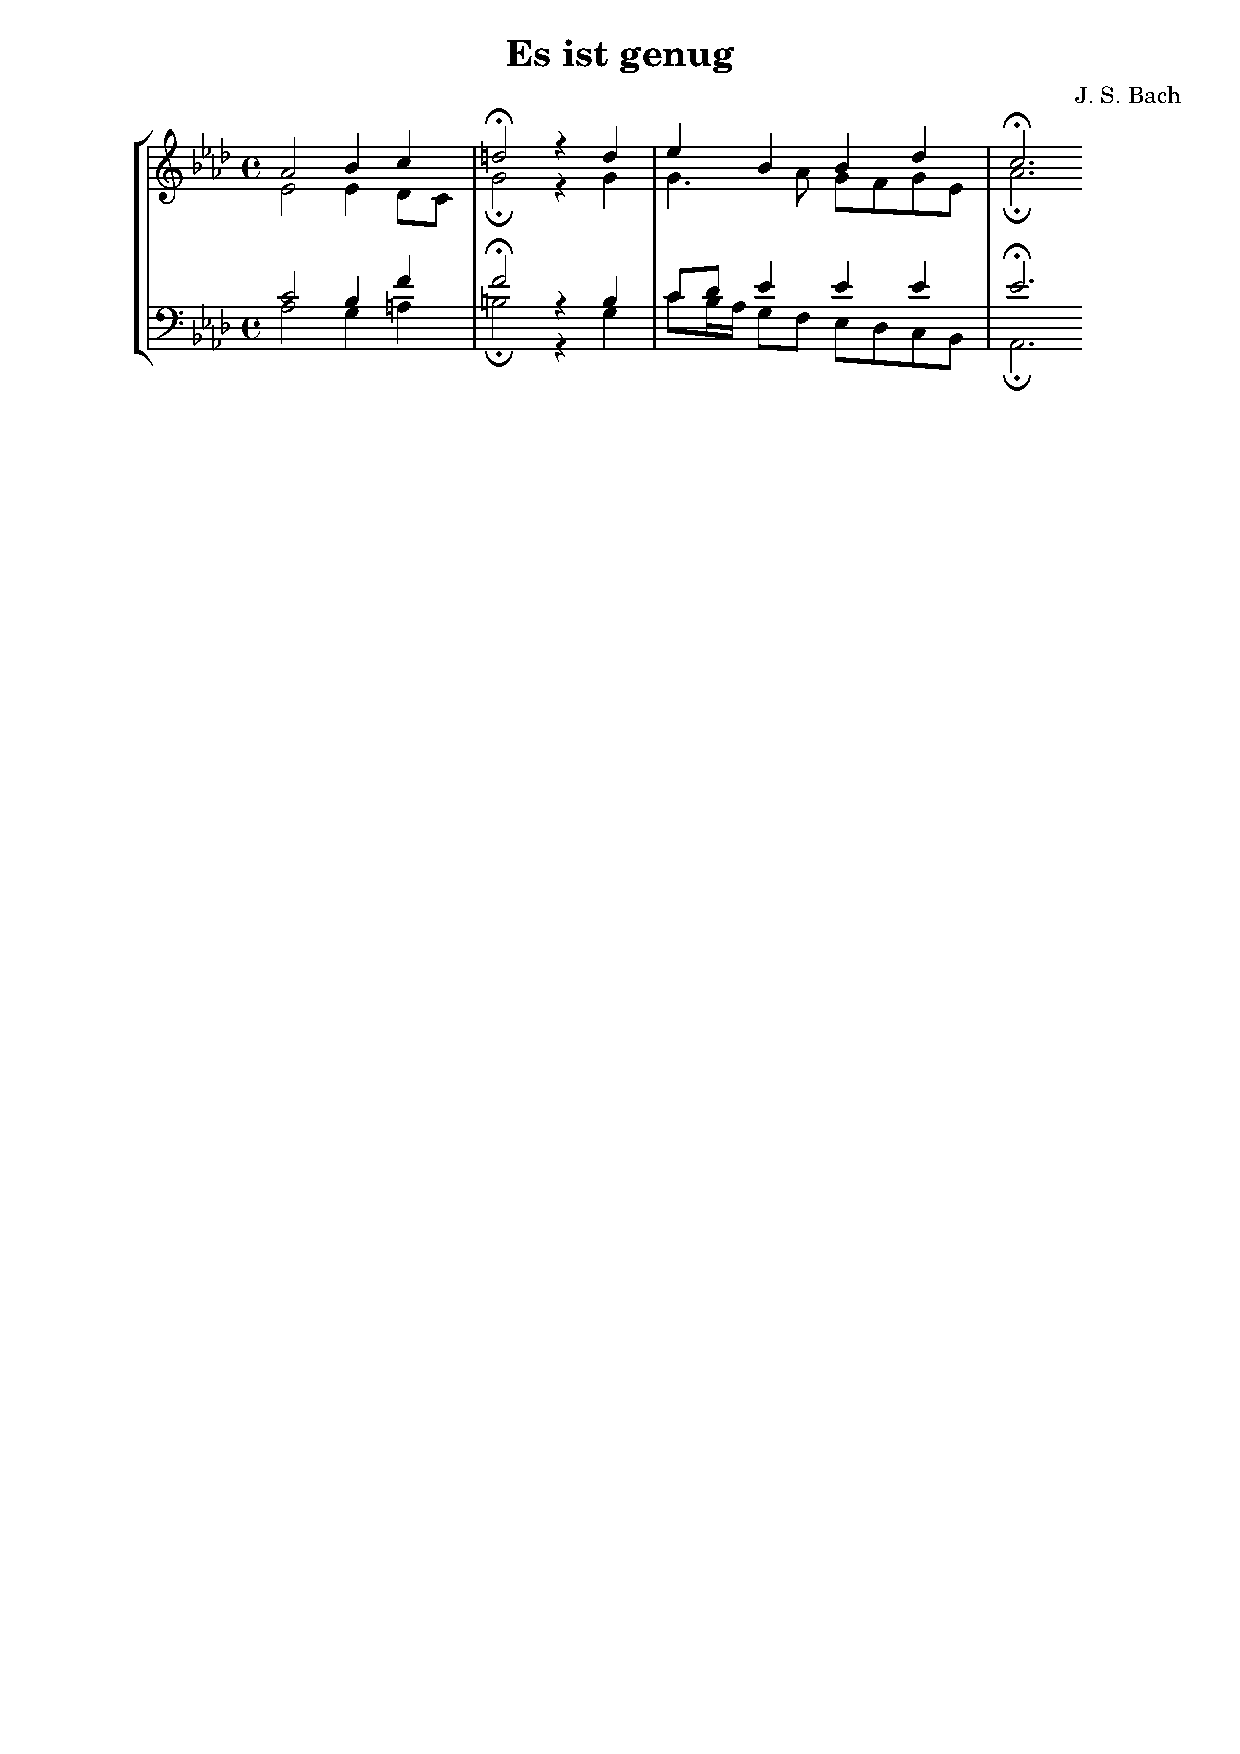
\includegraphics[scale=0.3875]{assets/example-es-ist-genug.pdf}
}
\end{multicols}
\end{singlespacing}

foo

\subsection{LaTeX}

foo

\begin{singlespacing}
\vspace{-0.5\baselineskip}
\begin{multicols}{2}
\lstinputlisting[style=beep]{assets/example-document.tex}
\vfill
\columnbreak
\setlength\fboxsep{0pt}
\setlength\fboxrule{0.5pt}
\noindent\fbox{
    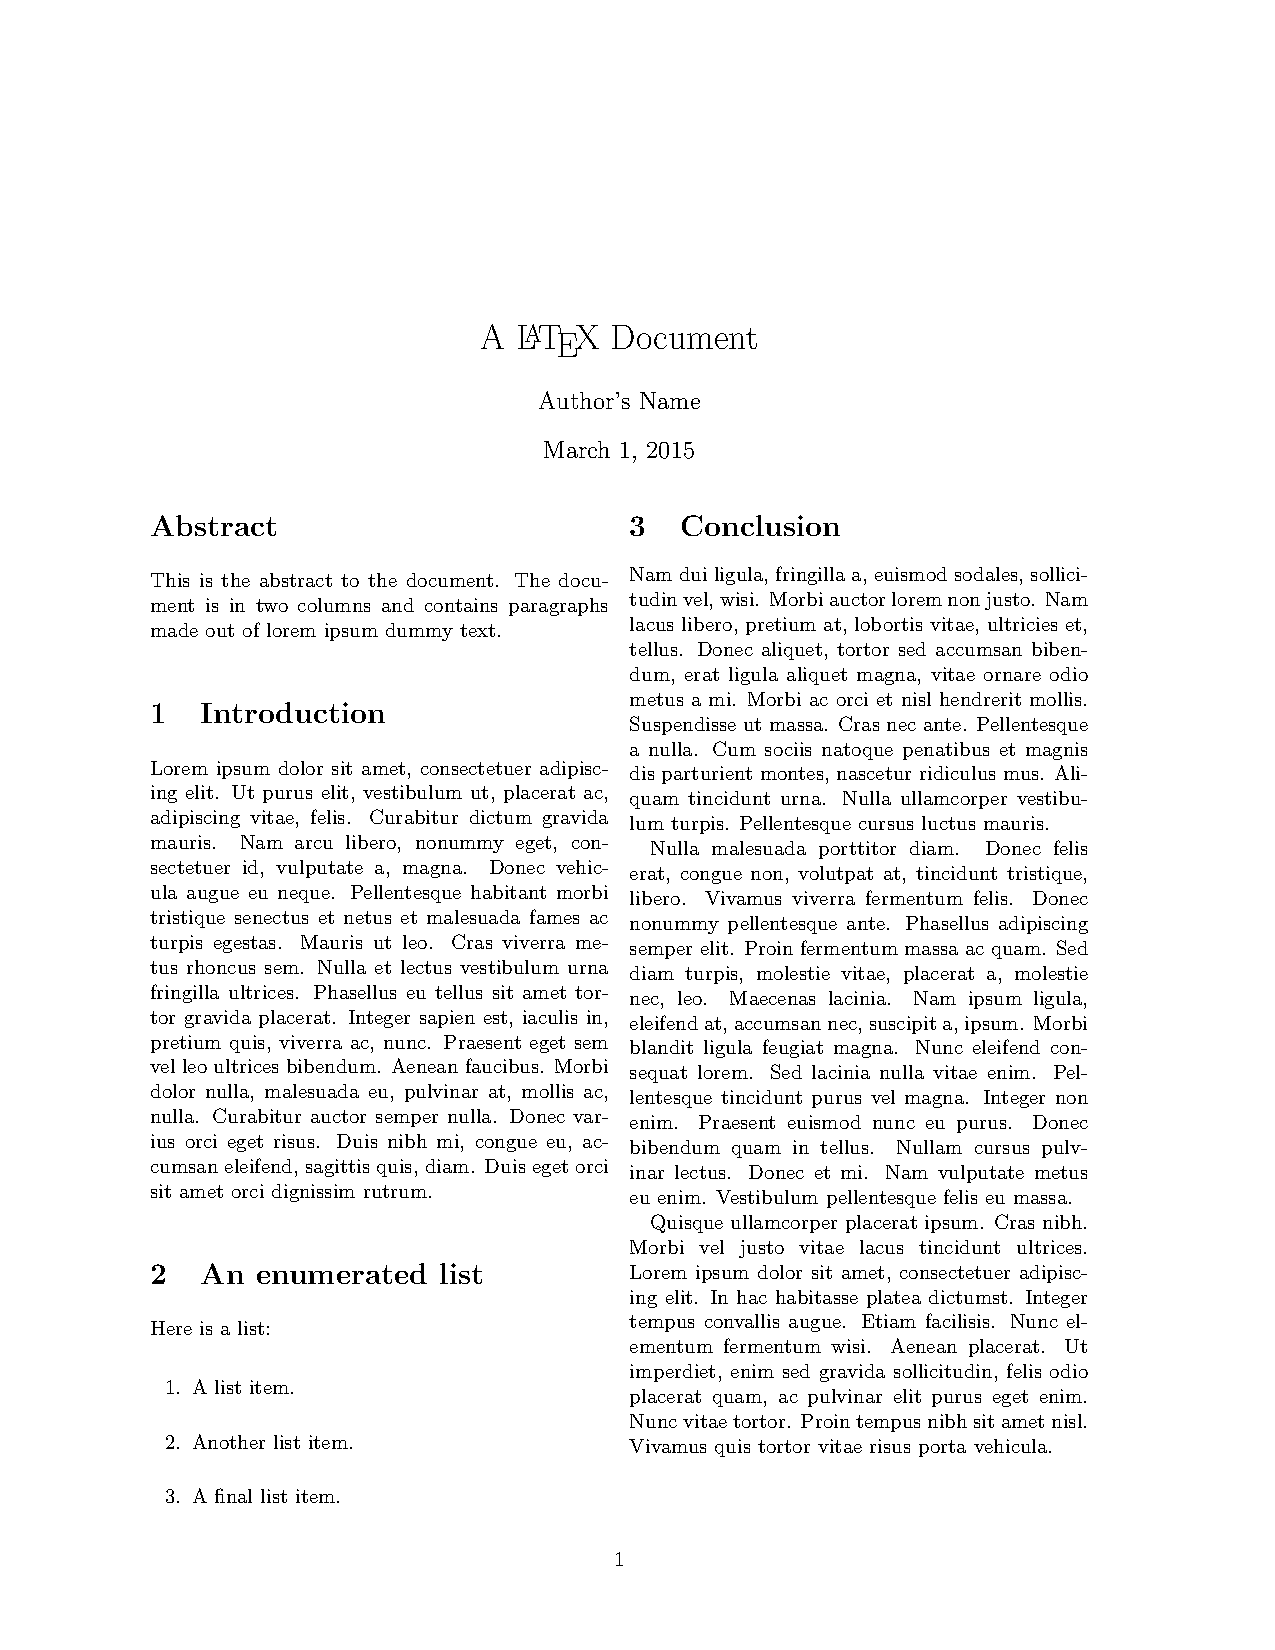
\includegraphics[scale=0.3875]{assets/example-document.pdf}
}
\end{multicols}
\end{singlespacing}

\subsection{Abjad}

foo

\subsection{Consort}

foo

%%%%%%%%%%%%%%%%%%%%%%%%%%%%%%%%%%%%%%%%%%%%%%%%%%%%%%%%%%%%%%%%%%%%%%%%%%%%%%%
\section{Motivation}
%%%%%%%%%%%%%%%%%%%%%%%%%%%%%%%%%%%%%%%%%%%%%%%%%%%%%%%%%%%%%%%%%%%%%%%%%%%%%%%

foo
%%%%%%%%%%%%%%%%%%%%%%%%%%%%%%%%%%%%%%%%%%%%%%%%%%%%%%%%%%%%%%%%%%%%%%%%%%%%%%%
\chapter{\emph{Abjad}: a model of notation}
\label{chap:a-model-of-notation}
%%%%%%%%%%%%%%%%%%%%%%%%%%%%%%%%%%%%%%%%%%%%%%%%%%%%%%%%%%%%%%%%%%%%%%%%%%%%%%%

Abjad\cite{baca2011xi, trevino2013compositional} is an open-source
Python\cite{vanrossum2003ys} package which extends the Python programming
language with a computational model of music notation. Abjad allows its users
to construct scores in an object-oriented fashion and visualize their work as
publication-quality notation at any point in the composition process.
Additionally, Abjad can be installed and imported into a Python interpreter
session just like any other Python package. Importantly, Abjad is not a
stand-alone application and has no GUI -- no graphic user interface -- unlike
many other related projects such as PWGL\cite{laurson2009qf,
kuuskankare2004recent}, OpenMusic\cite{assayag1999sw},
BACH\cite{agostini2013real} and many others. All work is done in the
command-line, either directly in an interactive Python console session, or by
writing modules of code to be imported into one another and executed by
Python's interpreter. Nearly all of the code examples in the body of this
document are presented as part of a single interactive Python console session
simply because Python's interactive console clearly distinguishes input from
output. Lines preceded by \texttt{>>>} will be passed to Python for
interpretation. Those preceded by \texttt{...} indicate the continuation of a
incomplete language construct. All other lines are necessarily returned as
output from Python's interpreter.

We can import Abjad into Python with the following incantation:

\begin{comment}
<abjad>
import abjad
</abjad>
\end{comment}

\begin{abjadbookoutput}
\begin{singlespacing}
\vspace{-0.5\baselineskip}
\begin{lstlisting}
>>> import abjad
\end{lstlisting}
\end{singlespacing}
\end{abjadbookoutput}

\noindent Abjad is implemented as a collection of over 900 public classes and
functions spread across nearly 40 subpackages, totally almost 200,000 lines of
source code. Many of these classes and functions are available immediately
within Abjad's root \emph{namespace}. We can enumerate these
\enquote{top-level} names by calling Python's built-in \texttt{dir()} function
on the imported \texttt{abjad} module object. After stripping out all
\enquote{private} names -- those starting with underscores -- Abjad's top-level
names can be printed to Python's interactive console:

\begin{comment}
<abjad>[text_width=105]
abjad_names = dir(abjad)
abjad_names = [x for x in abjad_names if not x.startswith('_')]
print(abjad_names)
</abjad>
\end{comment}

\begin{abjadbookoutput}
\begin{singlespacing}
\vspace{-0.5\baselineskip}
\begin{lstlisting}
>>> abjad_names = dir(abjad)
>>> abjad_names = [x for x in abjad_names if not x.startswith('_')]
>>> print(abjad_names)
['Accelerando', 'Articulation', 'Beam', 'Chord', 'Clef', 'Container', 'Context', 'Crescendo',
'Decrescendo', 'Duration', 'Dynamic', 'Fermata', 'Fraction', 'Glissando', 'Hairpin', 'KeySignature',
'Markup', 'Measure', 'MultimeasureRest', 'Multiplier', 'NamedPitch', 'Note', 'Offset', 'Rest',
'Ritardando', 'Score', 'Sequence', 'Skip', 'Slur', 'Staff', 'StaffGroup', 'Tempo', 'Tie',
'TimeSignature', 'Timespan', 'Tuplet', 'Voice', 'abctools', 'abjad_configuration', 'abjadbooktools',
'agenttools', 'attach', 'datastructuretools', 'detach', 'developerscripttools', 'documentationtools',
'durationtools', 'exceptiontools', 'f', 'graph', 'handlertools', 'indicatortools', 'inspect_',
'instrumenttools', 'ipythontools', 'iterate', 'labeltools', 'layouttools', 'lilypondfiletools',
'lilypondnametools', 'lilypondparsertools', 'markuptools', 'mathtools', 'metertools', 'mutate', 'new',
'override', 'parse', 'persist', 'pitchtools', 'play', 'quantizationtools', 'rhythmmakertools',
'rhythmtreetools', 'schemetools', 'scoretools', 'select', 'selectiontools', 'selectortools',
'sequencetools', 'set_', 'show', 'sievetools', 'spannertools', 'stringtools', 'systemtools',
'templatetools', 'timespantools', 'tonalanalysistools', 'topleveltools']
\end{lstlisting}
\end{singlespacing}
\end{abjadbookoutput}

\noindent Names beginning with uppercase letters represent classes. These
include many of the musical objects composers would likely create by hand. Most
of these classes have direct notational analogs on the page -- e.g.
\texttt{Note}, \texttt{Rest} and \texttt{Chord} --, or map to common structural
or typographic concepts in Abjad's primary typesetting engine, LilyPond, such
as \texttt{Voice}, \texttt{Markup} and \texttt{Skip}. Lowercase names ending in
the string \enquote{tools} represent additional libraries or \emph{subpackages}
within Abjad. These subpackages group together related functionality within a
common namespace. For example, Abjad's \texttt{pitchtools} subpackage contains
dozens of classes and functions solely for modeling pitch objects, collections
of those objects, and their transformations:

\begin{comment}
<abjad>[text_width=105]
pitchtools_names = dir(abjad.pitchtools)
pitchtools_names = [x for x in pitchtools_names if not x.startswith('_')]
print(pitchtools_names)
</abjad>
\end{comment}

\begin{abjadbookoutput}
\begin{singlespacing}
\vspace{-0.5\baselineskip}
\begin{lstlisting}
>>> pitchtools_names = dir(abjad.pitchtools)
>>> pitchtools_names = [x for x in pitchtools_names if not x.startswith('_')]
>>> print(pitchtools_names)
['Accidental', 'Interval', 'IntervalClass', 'IntervalClassSegment', 'IntervalClassSet',
'IntervalClassVector', 'IntervalSegment', 'IntervalSet', 'IntervalVector', 'Inversion', 'Multiplication',
'NamedInterval', 'NamedIntervalClass', 'NamedInversionEquivalentIntervalClass', 'NamedPitch',
'NamedPitchClass', 'NumberedInterval', 'NumberedIntervalClass',
'NumberedInversionEquivalentIntervalClass', 'NumberedPitch', 'NumberedPitchClass',
'NumberedPitchClassColorMap', 'Octave', 'Pitch', 'PitchArray', 'PitchArrayCell', 'PitchArrayColumn',
'PitchArrayInventory', 'PitchArrayRow', 'PitchClass', 'PitchClassSegment', 'PitchClassSet',
'PitchClassTree', 'PitchClassVector', 'PitchOperation', 'PitchRange', 'PitchRangeInventory',
'PitchSegment', 'PitchSet', 'PitchVector', 'Registration', 'RegistrationComponent',
'RegistrationInventory', 'Retrogression', 'Rotation', 'Segment', 'Set', 'StaffPosition', 'Transposition',
'TwelveToneRow', 'Vector', 'instantiate_pitch_and_interval_test_collection',
'inventory_inversion_equivalent_named_interval_classes',
'inventory_named_inversion_equivalent_interval_classes', 'iterate_named_pitch_pairs_in_expr',
'list_named_pitches_in_expr', 'list_numbered_interval_numbers_pairwise',
'list_numbered_inversion_equivalent_interval_classes_pairwise',
'list_ordered_named_pitch_pairs_from_expr_1_to_expr_2', 'list_pitch_numbers_in_expr',
'list_unordered_named_pitch_pairs_in_expr', 'set_written_pitch_of_pitched_components_in_expr',
'sort_named_pitch_carriers_in_expr', 'transpose_named_pitch_by_numbered_interval_and_respell',
'transpose_pitch_carrier_by_interval', 'transpose_pitch_class_number_to_pitch_number_neighbor',
'transpose_pitch_expr_into_pitch_range', 'transpose_pitch_number_by_octave_transposition_mapping',
'yield_all_pitch_class_sets']
\end{lstlisting}
\end{singlespacing}
\end{abjadbookoutput}

\noindent Many of these subpackages implement opinionated collections of
compositional devices, certainly useful for some composers but by no means
considered core to Abjad's notational model. For example, Abjad's
\texttt{quantizationtools} provides a rhythmic quantizer inspired by Paul
Nauert's concept of \enquote{Q-grids}\cite{nauert1997timespan},
\texttt{rhythmtreetools} parses a Lisp-like \enquote{RTM-syntax} -- which
should be familiar to anyone working with OpenMusic\cite{assayag1999sw},
PWGL\cite{laurson2009qf, kuuskankare2004recent} or Bach\cite{agostini2013real},
-- into object-oriented rhythm-tree data structures, and the
\texttt{sievetools} subpackage models Iannis Xenakis' pitch
sieves\cite{xenakis1992formalized}. Still other subpackages implement more
\enquote{objective} functionality, such as \texttt{mathtools} or
\texttt{durationtools}. Many of the remaining subpackages collect together
related musical and typographic classes and functions, e.g.
\texttt{scoretools}, \texttt{spannertools}, \texttt{markuptools}, and
\texttt{indicatortools}. Others simply exist for \enquote{internal} use by
Abjad's developers, assisting in the development and maintenance of the system,
such as \texttt{abctools}, \texttt{developerscripttools},
\texttt{documentationtools} and \texttt{systemtools}.

The remaining names in Abjad's namespace represent its \enquote{top-level}
functions, including \texttt{attach()}, \texttt{detach()},
\texttt{inspect\_()}, \texttt{iterate()}, \texttt{mutate()}, \texttt{new()},
\texttt{override()}, \texttt{parse()}, \texttt{persist()}, \texttt{play()},
\texttt{select()}, \texttt{set\_()}, and -- most importantly --
\texttt{show()}. These functions provide a powerful set of tools for
interacting with Abjad's notational objects and factories, and will be
explained in detail as we encounter each of them.

For the sake of brevity, this document -- across each chapter -- will behave as
though the contents of Abjad's namespace has been imported into Python's global
namespace:

\begin{comment}
<abjad>
from abjad import *
</abjad>
\end{comment}

\begin{abjadbookoutput}
\begin{singlespacing}
\vspace{-0.5\baselineskip}
\begin{lstlisting}
>>> from abjad import *
\end{lstlisting}
\end{singlespacing}
\end{abjadbookoutput}

\section{Representing objects}

In Python, everything is an object, even integers, boolean values and
functions. Because Python is also interpreted and can be used interactively,
those objects must be representable in an interpreter session, which is
necessarily textual. Objects' text, or \emph{string}, representations can take
a variety of forms, and those same objects may specify explicitly how they
should be represented textually, just as they may specify how they should
behave in relation to operations such as addition, multiplication, or
iteration.

Python classes often specify their behavior in terms of \emph{protocols}.
Protocols are established by convention rather than enforced at the system
level. This explanation takes place via \enquote{dunder} methods --
double-underscore methods -- such as \texttt{\_\_repr\_\_()} which provides an
object's \emph{interpreter representation} in cooperation with Python's
\texttt{repr()} function and \texttt{\_\_str\_\_()} which provides an object's
string representation in cooperation with Python's \texttt{str()}
function. By overriding these dunder methods, a class may specify its own
version of string or interpreter representation behavior.

For example, a simple \texttt{Foo} class, which overrides neither
\texttt{\_\_str\_\_()} nor \texttt{\_\_repr\_\_()} may be defined and
instantiated:

\begin{comment}
<abjad>
class Foo(object):
    pass

foo = Foo()
</abjad>
\end{comment}

\begin{abjadbookoutput}
\begin{singlespacing}
\vspace{-0.5\baselineskip}
\begin{lstlisting}
>>> class Foo(object):
...     pass
...
>>> foo = Foo()
\end{lstlisting}
\end{singlespacing}
\end{abjadbookoutput}

\noindent When printed to the terminal, cast as a string, and represented,
Python's default object representation is used, giving the module and name of
the class as well as its memory location. Note that when calling Python's
\texttt{print()} function on an object, that object is converted to a string
and then printed to the console, resulting in text without quotation marks:

\begin{comment}
<abjad>
print(foo)
repr(foo)
str(foo)
</abjad>
\end{comment}

\begin{abjadbookoutput}
\begin{singlespacing}
\vspace{-0.5\baselineskip}
\begin{lstlisting}
>>> print(foo)
<__main__.Foo object at 0x10392e590>
\end{lstlisting}
\begin{lstlisting}
>>> repr(foo)
'<__main__.Foo object at 0x10392e590>'
\end{lstlisting}
\begin{lstlisting}
>>> str(foo)
'<__main__.Foo object at 0x10392e590>'
\end{lstlisting}
\end{singlespacing}
\end{abjadbookoutput}

\noindent Defining a new class, \texttt{Foo2}, which overrides both string and
interpreter representation provides customized output. Note that printing the
\texttt{Foo2} instance relies on its string representation, rather than its
interpreter representation, while simply referencing the instantiated
\texttt{Foo2} object uses its interpreter representation -- its \enquote{repr}:

\begin{comment}
<abjad>
class Foo2(object):
    def __repr__(self):
        return '<I am Foo2>'
    def __str__(self):
        return 'foofoo'

foo2 = Foo2()
foo2
print(foo2)
repr(foo2)
str(foo2)
</abjad>
\end{comment}

\begin{abjadbookoutput}
\begin{singlespacing}
\vspace{-0.5\baselineskip}
\begin{lstlisting}
>>> class Foo2(object):
...     def __repr__(self):
...         return '<I am Foo2>'
...     def __str__(self):
...         return 'foofoo'
...
>>> foo2 = Foo2()
>>> foo2
<I am Foo2>
\end{lstlisting}
\begin{lstlisting}
>>> print(foo2)
foofoo
\end{lstlisting}
\begin{lstlisting}
>>> repr(foo2)
'<I am Foo2>'
\end{lstlisting}
\begin{lstlisting}
>>> str(foo2)
'foofoo'
\end{lstlisting}
\end{singlespacing}
\end{abjadbookoutput}

\noindent Defining a third version of \texttt{Foo} with an overridden
\texttt{\_\_format\_\_()} method allows for creating alternate string
representations. By calling Python's built-in \texttt{format()} function on a
\texttt{Foo3} instance, either the normal string representation or a
\enquote{special} representation can be created. This formatting behavior can
also be extended to support an arbitrary number of format specifications:

\begin{comment}
<abjad>
class Foo3(object):
    def __format__(self, format_specification=''):
        if format_specification == 'special':
            return '~~~ special foo format ~~~~'
        return str(self)
    def __repr__(self):
        return '<I am Foo3>'
    def __str__(self):
        return 'foofoofoo'

foo3 = Foo3()
foo3
print(foo3)
repr(foo3)
str(foo3)
format(foo3)
format(foo3, 'special')
</abjad>
\end{comment}

\begin{abjadbookoutput}
\begin{singlespacing}
\vspace{-0.5\baselineskip}
\begin{lstlisting}
>>> class Foo3(object):
...     def __format__(self, format_specification=''):
...         if format_specification == 'special':
...             return '~~~ special foo format ~~~~'
...         return str(self)
...     def __repr__(self):
...         return '<I am Foo3>'
...     def __str__(self):
...         return 'foofoofoo'
...
>>> foo3 = Foo3()
>>> foo3
<I am Foo3>
\end{lstlisting}
\begin{lstlisting}
>>> print(foo3)
foofoofoo
\end{lstlisting}
\begin{lstlisting}
>>> repr(foo3)
'<I am Foo3>'
\end{lstlisting}
\begin{lstlisting}
>>> str(foo3)
'foofoofoo'
\end{lstlisting}
\begin{lstlisting}
>>> format(foo3)
'foofoofoo'
\end{lstlisting}
\begin{lstlisting}
>>> format(foo3, 'special')
'~~~ special foo format ~~~~'
\end{lstlisting}
\end{singlespacing}
\end{abjadbookoutput}

\noindent Many Abjad objects have multiple possible string representations. For
example, a \texttt{Note} object can be represented by its normal interpreter
representation, as a LilyPond string, or by its \emph{storage format} -- a more
verbose, potentially multi-line string representation generally used when
persisting complex objects to disk.

\begin{comment}
<abjad>
note = Note(NamedPitch("g'"), Duration(3, 4))
note
print(repr(note))
print(note)
print(str(note))
print(format(note))
print(format(note, 'lilypond'))
print(format(note, 'storage'))
</abjad>
\end{comment}

\begin{abjadbookoutput}
\begin{singlespacing}
\vspace{-0.5\baselineskip}
\begin{lstlisting}
>>> note = Note(NamedPitch("g'"), Duration(3, 4))
>>> note
Note("g'2.")
\end{lstlisting}
\begin{lstlisting}
>>> print(repr(note))
Note("g'2.")
\end{lstlisting}
\begin{lstlisting}
>>> print(note)
g'2.
\end{lstlisting}
\begin{lstlisting}
>>> print(str(note))
g'2.
\end{lstlisting}
\begin{lstlisting}
>>> print(format(note))
g'2.
\end{lstlisting}
\begin{lstlisting}
>>> print(format(note, 'lilypond'))
g'2.
\end{lstlisting}
\begin{lstlisting}
>>> print(format(note, 'storage'))
scoretools.Note("g'2.")
\end{lstlisting}
\end{singlespacing}
\end{abjadbookoutput}

\noindent For some Abjad classes -- especially those representing glyphs in
music notation -- their default string format is their LilyPond string
representation. Other classes -- especially Abjad's various highly-configurable
notation factory classes -- default their string format to their storage
format, allowing for complex but still human-readable interpreter output:

\begin{comment}
<abjad>
rhythm_maker = rhythmmakertools.TaleaRhythmMaker(
    talea=rhythmmakertools.Talea([1, 2, 3], 16),
    extra_counts_per_division=(1, 0, 2, 1, 0),
    output_masks=[
        rhythmmakertools.SustainMask([1], 3, 1, -1),
        rhythmmakertools.SilenceMask([-1]),
        ],
    tie_specifier=rhythmmakertools.TieSpecifier(
        tie_across_divisions=True,
        ),
    )
print(format(rhythm_maker))
</abjad>
\end{comment}

\begin{abjadbookoutput}
\begin{singlespacing}
\vspace{-0.5\baselineskip}
\begin{lstlisting}
>>> rhythm_maker = rhythmmakertools.TaleaRhythmMaker(
...     talea=rhythmmakertools.Talea([1, 2, 3], 16),
...     extra_counts_per_division=(1, 0, 2, 1, 0),
...     output_masks=[
...         rhythmmakertools.SustainMask([1], 3, 1, -1),
...         rhythmmakertools.SilenceMask([-1]),
...         ],
...     tie_specifier=rhythmmakertools.TieSpecifier(
...         tie_across_divisions=True,
...         ),
...     )
>>> print(format(rhythm_maker))
rhythmmakertools.TaleaRhythmMaker(
    talea=rhythmmakertools.Talea(
        counts=(1, 2, 3),
        denominator=16,
        ),
    extra_counts_per_division=(1, 0, 2, 1, 0),
    output_masks=rhythmmakertools.BooleanPatternInventory(
        (
            rhythmmakertools.SustainMask(
                indices=(1,),
                period=3,
                start=1,
                stop=-1,
                ),
            rhythmmakertools.SilenceMask(
                indices=(-1,),
                ),
            )
        ),
    tie_specifier=rhythmmakertools.TieSpecifier(
        tie_across_divisions=True,
        ),
    )
\end{lstlisting}
\end{singlespacing}
\end{abjadbookoutput}

\noindent Finally, in the spirit of Python's protocols and dunder conventions,
Abjad provides its own \emph{illustration protocol} and
\texttt{\_\_illustrate\_\_()} dunder method. This method works with Abjad's
top-level \texttt{show()} function to generate graphic realizations of
illustratable Python objects via LilyPond. Abjad's \texttt{show()} function
will be used throughout this document to create and display notation and
otherwise graphic representations:

\begin{comment}
<abjad>
show(note)
</abjad>
\end{comment}

\begin{abjadbookoutput}
\begin{singlespacing}
\vspace{-0.5\baselineskip}
\begin{lstlisting}
>>> show(note)
\end{lstlisting}
\noindent\includegraphics[max width=\textwidth,]{assets/lilypond-5cfff2844553f774341de4a66c379061.pdf}
\end{singlespacing}
\end{abjadbookoutput}

\section{Components}

\begin{comment}
-   Every component may be named.
-   components, leaves, containers (and contexts)
-   components are formattable and illustrable
-   components are mutable, while indicators are generally not
    -   likewise, durations and pitches are immutable

-   count-time components
    -   note, chord, rest, skip, container, tuplet, measure
-   non-count-time (contexts)
    -   voice, staff, staff group, score

-   leaves do not contain anything else
    -   chord do *not* contain notes
    -   chords and notes contain note heads
    -   chord and notes share a single stem
    -   this must be disambiguated from note columns

-   all containers derive their duration from their contents (with some
    exceptions, but even there a mismatch is an error)
-   written duration, prolated duration, pre-prolated duration, contents
    duration

-   One, and only one, parent per component. They *cannot* be in more than one
    container. This is both confusing, and liable to cause reference problems.
-   score hierarchy is not fixed: any node is the root, if it has no parent

-   contexts are assumed to last from the beginning to the end of the total
    timespan of the score, but in practice they may be intermittent
-   contexts may be named, allowing concatenation

-   Leaves reside at the "bottom" of the score hierarchy.

Work aspects of this into appropriate sections

-   inspect_()
-   not *inspect()*, as that would cause a name conflict with Python's inspect
    module
-   inspect(...).get_parentage()
-   inspect_(...).get_duration()
    -   in_seconds=True
-   inspect_(...).get_timespan()
    -   in_seconds=True
\end{comment}

Abjad models notated musical scores as a \emph{tree} consisting of
\emph{components}, \emph{indicators} and \emph{spanners}. All objects appearing
in a score fall into one of those three categories. The most important and most
complex of the three groups, components, make up the \emph{nodes} of the score
tree, treating the score as an acyclic directed rooted graph, or
\emph{arborescence}, rooted on a single component. All components inherit from
Abjad's \texttt{Component} class, which encapsulates logic crucial to
maintaining the correctness of the score tree, and affords behaviors common to
all component subclasses including illustration, formatting and naming. Abjad
divides score components into \emph{containers} -- those components which may
contain other other components, such as staves, voices, tuplets, measures and
so forth -- and \emph{leaves} -- those components which may contain no other
components, such as notes, chords and rests, as well as LilyPond's
multi-measure rests and non-printing typographic \emph{skips}. Additionally,
components can each be instantiated from a variety of input, from parsable
LilyPond syntax strings to parametric arguments -- both numeric and explicitly
object-modeled via pitch and duration objects. For example, we can instantiate
and illustrate a middle-C quarter note:

\begin{comment}
<abjad>
note = Note("c'4")
show(note)
</abjad>
\end{comment}

\begin{abjadbookoutput}
\begin{singlespacing}
\vspace{-0.5\baselineskip}
\begin{lstlisting}
>>> note = Note("c'4")
>>> show(note)
\end{lstlisting}
\noindent\includegraphics[max width=\textwidth,]{assets/lilypond-c018a545d264ff34225e9a3a5babb6c1.pdf}
\end{singlespacing}
\end{abjadbookoutput}

\noindent a half-note rest:

\begin{comment}
<abjad>
rest = Rest((1, 2))
show(rest)
</abjad>
\end{comment}

\begin{abjadbookoutput}
\begin{singlespacing}
\vspace{-0.5\baselineskip}
\begin{lstlisting}
>>> rest = Rest((1, 2))
>>> show(rest)
\end{lstlisting}
\noindent\includegraphics[max width=\textwidth,]{assets/lilypond-8144dc38435e18921a5d584ad635d2e3.pdf}
\end{singlespacing}
\end{abjadbookoutput}

\noindent and a D-minor chord:

\begin{comment}
<abjad>
chord = Chord(
    [NamedPitch("d'"), NamedPitch("f'"), NamedPitch("a'")],
    Duration(1, 4),
    )
show(chord)
</abjad>
\end{comment}

\begin{abjadbookoutput}
\begin{singlespacing}
\vspace{-0.5\baselineskip}
\begin{lstlisting}
>>> chord = Chord(
...     [NamedPitch("d'"), NamedPitch("f'"), NamedPitch("a'")],
...     Duration(1, 4),
...     )
>>> show(chord)
\end{lstlisting}
\noindent\includegraphics[max width=\textwidth,]{assets/lilypond-fef850f162448b1e8d3c6be53e362436.pdf}
\end{singlespacing}
\end{abjadbookoutput}

\noindent Each of the above three leaf instantiations demonstrates a different
means of creating score objects, none of which is unique to the particular
class they have been demonstrated with here. The \texttt{Note} instantiation
demonstrates creating a score object via LilyPond syntax, the rest
instantiation demonstrates creating a score object from
sequences of integers -- in this case the pair (1, 2), representing the
duration of a half-note -- and the chord instantiation demonstrates using
explicit \texttt{NamedPitch} and \texttt{Duration} objects. The latter two
instantiation techniques afford parametric approaches, while the LilyPond
syntax allows for a great degree of expressivity as score components can be
created with articulations, dynamics and other indicators already attached:

\begin{comment}
<abjad>
fancy_chord = Chord(r"<g' bf'? d''>4. -\accent -\staccato ^\markup{ \italic gently }")
show(fancy_chord)
</abjad>
\end{comment}

\begin{abjadbookoutput}
\begin{singlespacing}
\vspace{-0.5\baselineskip}
\begin{lstlisting}
>>> fancy_chord = Chord(r"<g' bf'? d''>4. -\accent -\staccato ^\markup{ \italic gently }")
>>> show(fancy_chord)
\end{lstlisting}
\noindent\includegraphics[max width=\textwidth,]{assets/lilypond-ffbf3288650db529c52c1e9ac804f9f0.pdf}
\end{singlespacing}
\end{abjadbookoutput}

\subsection{Containers}
\label{ssec:containers}

Abjad's container classes -- measures, tuplets, voice, staves, staff groups,
scores and so forth -- implement Python's \emph{mutable sequence protocol},
allowing them to be used transparently as though they were lists.

Components can be appended, extended, or inserted into a container, and
container can be instantiated with lists of components to be contained as one
of their arguments. Note above that the LilyPond output shows a \sfrac{4}{4}
time signature even though none of the created leaves takes up an whole note's
duration. LilyPond simply treats all music as \sfrac{4}{4} unless explicitly
instructed otherwise. We can make the \sfrac{4}{4} time signature explicit by
instantiating a \sfrac{4}{4} measure to contain the previously-created three
leaf instances:

\begin{comment}
<abjad>
measure = Measure((4, 4), [note, rest, chord])
show(measure)
</abjad>
\end{comment}

\begin{abjadbookoutput}
\begin{singlespacing}
\vspace{-0.5\baselineskip}
\begin{lstlisting}
>>> measure = Measure((4, 4), [note, rest, chord])
>>> show(measure)
\end{lstlisting}
\noindent\includegraphics[max width=\textwidth,]{assets/lilypond-cad7b59ce37e423c6cdc4729377818c7.pdf}
\end{singlespacing}
\end{abjadbookoutput}

\noindent Containers can also be indexed into, measured for length and iterated
over. For example, the second component contained by the measure can be
retrieved by subscripting the measure with the index 1:

\begin{comment}
<abjad>
measure[1]
</abjad>
\end{comment}

\begin{abjadbookoutput}
\begin{singlespacing}
\vspace{-0.5\baselineskip}
\begin{lstlisting}
>>> measure[1]
Rest('r2')
\end{lstlisting}
\end{singlespacing}
\end{abjadbookoutput}

\noindent That second component -- the half-note rest -- can be replaced by
another container, a triplet:

\begin{comment}
<abjad>
outer_tuplet = Tuplet((2, 3), "a'4 b4 cs'4")
measure[1] = outer_tuplet
show(measure)
</abjad>
\end{comment}

\begin{abjadbookoutput}
\begin{singlespacing}
\vspace{-0.5\baselineskip}
\begin{lstlisting}
>>> outer_tuplet = Tuplet((2, 3), "a'4 b4 cs'4")
>>> measure[1] = outer_tuplet
>>> show(measure)
\end{lstlisting}
\noindent\includegraphics[max width=\textwidth,]{assets/lilypond-f9a8a92bd9dbe5f480a4003ade9c81aa.pdf}
\end{singlespacing}
\end{abjadbookoutput}

\noindent Furthermore, the last two leaves in the triplet can be replaced by a
quintuplet using Python's \emph{slice assignment} syntax. In the following
code, the text \texttt{outer\_tuplet[1:]} references the selection of
components in the original triplet starting from the second component and going
\enquote{to the end} -- effectively the second and third item, as there are
only three. That selection is then replaced by a list containing a quintuplet,
substituting the contents of one sequence of components for the contents of
another.

\begin{comment}
<abjad>
inner_tuplet = Tuplet((4, 5), "b'8 a'8. g'16 f'32 e'8..")
outer_tuplet[1:] = [inner_tuplet]
show(measure)
</abjad>
\end{comment}

\begin{abjadbookoutput}
\begin{singlespacing}
\vspace{-0.5\baselineskip}
\begin{lstlisting}
>>> inner_tuplet = Tuplet((4, 5), "b'8 a'8. g'16 f'32 e'8..")
>>> outer_tuplet[1:] = [inner_tuplet]
>>> show(measure)
\end{lstlisting}
\noindent\includegraphics[max width=\textwidth,]{assets/lilypond-b783a8dad0c3003152ef1b148bc60ca8.pdf}
\end{singlespacing}
\end{abjadbookoutput}

\noindent The measure can be inspected for its length by using Python's
built-in \texttt{len()} function. Note that this returns the number of
components \emph{immediately} contained by the measure -- 3 --, but not the
total number of components, total number of leaves or total duration. The
latter queries can be satisfied by other means.

\begin{comment}
<abjad>
len(measure)
</abjad>
\end{comment}

\begin{abjadbookoutput}
\begin{singlespacing}
\vspace{-0.5\baselineskip}
\begin{lstlisting}
>>> len(measure)
3
\end{lstlisting}
\end{singlespacing}
\end{abjadbookoutput}

\noindent Iterating over the contents of the \sfrac{4}{4} measure yields only
the top-most components in that container -- its immediate children:

\begin{comment}
<abjad>
for component in measure:
    component

</abjad>
\end{comment}

\begin{abjadbookoutput}
\begin{singlespacing}
\vspace{-0.5\baselineskip}
\begin{lstlisting}
>>> for component in measure:
...     component
...
Note("c'4")
Tuplet(Multiplier(2, 3), "a'4 { 4/5 b'8 a'8. g'16 f'32 e'8.. }")
Chord("<d' f' a'>4")
\end{lstlisting}
\end{singlespacing}
\end{abjadbookoutput}

\noindent To retrieve all of the leaves of a container, recursion must be used,
as any container may contain other containers, and those in turn still more
containers. To mitigate this complexity, every container provides a
\texttt{select\_leaves()} method, which returns a selection of the bottom-most
leaf instances in the subtree rooted at that container:

\begin{comment}
<abjad>
for leaf in measure.select_leaves():
    leaf

</abjad>
\end{comment}

\begin{abjadbookoutput}
\begin{singlespacing}
\vspace{-0.5\baselineskip}
\begin{lstlisting}
>>> for leaf in measure.select_leaves():
...     leaf
...
Note("c'4")
Note("a'4")
Note("b'8")
Note("a'8.")
Note("g'16")
Note("f'32")
Note("e'8..")
Chord("<d' f' a'>4")
\end{lstlisting}
\end{singlespacing}
\end{abjadbookoutput}

\noindent Note that Abjad's \texttt{Chord} class aggregates multiple \emph{note
heads} rather than notes. Likewise Abjad's \texttt{Note} class aggregates a
single note head. While chords implement containment in terms of note heads --
delegating to a dedicated note head inventory -- they are not themselves
"containers" in the same sense that a voice, measure or tuplet are containers.
It is important here to differentiate between the concept of a \enquote{chord}
as a single duration paired with a collection of pitches and a \enquote{chord}
as the sounding sonority at some given point in a piece spread over some number
of voices. Abjad always makes use of the former rather than the latter.

\begin{comment}
<abjad>
note_head_inventory = chord.note_heads
for note_head in note_head_inventory:
    note_head

chord.note_heads.append(NamedPitch("c''"))
show(chord)
</abjad>
\end{comment}

\begin{abjadbookoutput}
\begin{singlespacing}
\vspace{-0.5\baselineskip}
\begin{lstlisting}
>>> note_head_inventory = chord.note_heads
>>> for note_head in note_head_inventory:
...     note_head
...
NoteHead("d'")
NoteHead("f'")
NoteHead("a'")
\end{lstlisting}
\begin{lstlisting}
>>> chord.note_heads.append(NamedPitch("c''"))
>>> show(chord)
\end{lstlisting}
\noindent\includegraphics[max width=\textwidth,]{assets/lilypond-0419b405f12cba5bff2e20c17c72e860.pdf}
\end{singlespacing}
\end{abjadbookoutput}

\subsection{Parentage}
\label{ssec:parentage}

The container that contains a given component is called its \emph{parent}, and
the components contained in a container are known as that container's
\emph{children}. Every component may have one and only one parent container,
although a component may also have no parent -- a null parent reference. Any
component whose parent is null is necessarily the root of its own score tree.
Furthermore, no component may appear in its own \emph{proper parentage} -- the
sequence of components comprising the unique path from a given component to the
root of its tree, excepting the component itself -- as this would induce
reference cycles within the score tree.\footnote{Disambiguate proper and
improper parentage in terms of set-theory.}

Abjad object-models the concept of parentage explicitly as a \texttt{Parentage}
\emph{selection} class, accessible via the \emph{inspector} which exposes a
given component's \emph{inspection interface}: a collection of methods for
accessing information about that component, many of which depend on that
component's position within the score hierarchy, including the component's
parentage or duration. An inspector can be instantiated by calling Abjad's
top-level \texttt{inspect\_()} function on a component.\footnote{Abjad uses
\texttt{inspect\_()} rather than \texttt{inspect()} as Python already provides
an \texttt{inspect} module for object introspection, and it is considered bad
practice to overwrite names of functions, classes or modules found in the
standard library such as \texttt{set} or \texttt{object}. When a name conflict
would occur, projects traditionally append an underscore to the name they wish
to use.} Consider the parentage for the first eighth note of the inner tuplet.
Its parentage -- \emph{improper} by default -- includes itself, its immediate
quintuplet parent, its triplet grandparent and the \sfrac{4}{4} measure as its
great-grandparent:\footnote{The component summary strings in the interpreter
representations of the components in the parentage are \emph{note} valid
LilyPond syntax, but simply a concise LilyPond-like syntax.}

\begin{comment}
<abjad>
inner_b_eighth = measure[1][1][0]
inspector = inspect_(inner_b_eighth)
parentage = inspector.get_parentage()
parentage.parent
for component in parentage:
    component

</abjad>
\end{comment}

\begin{abjadbookoutput}
\begin{singlespacing}
\vspace{-0.5\baselineskip}
\begin{lstlisting}
>>> inner_b_eighth = measure[1][1][0]
>>> inspector = inspect_(inner_b_eighth)
>>> parentage = inspector.get_parentage()
>>> parentage.parent
Tuplet(Multiplier(4, 5), "b'8 a'8. g'16 f'32 e'8..")
\end{lstlisting}
\begin{lstlisting}
>>> for component in parentage:
...     component
...
Note("b'8")
Tuplet(Multiplier(4, 5), "b'8 a'8. g'16 f'32 e'8..")
Tuplet(Multiplier(2, 3), "a'4 { 4/5 b'8 a'8. g'16 f'32 e'8.. }")
Measure((4, 4), "c'4 { 2/3 a'4 { 4/5 b'8 a'8. g'16 f'32 e'8.. } } <d' f' a' c''>4")
\end{lstlisting}
\end{singlespacing}
\end{abjadbookoutput}

\noindent By default, every component's parent is null, represented in Python
by Python's \texttt{None} object:

\begin{comment}
<abjad>
whole_note = Note("c'1")
inspector = inspect_(whole_note)
inspector.get_parentage().parent is None
</abjad>
\end{comment}

\begin{abjadbookoutput}
\begin{singlespacing}
\vspace{-0.5\baselineskip}
\begin{lstlisting}
>>> whole_note = Note("c'1")
>>> inspector = inspect_(whole_note)
>>> inspector.get_parentage().parent is None
True
\end{lstlisting}
\end{singlespacing}
\end{abjadbookoutput}

\noindent Inserting the above whole note into a container sets the whole note's
parent to that container. Additionally, the container is now aware that it
contains the whole note, demonstrating the bi-directional references inherent
to Abjad's score tree model:

\begin{comment}
<abjad>
container_one = Container()
container_one.append(whole_note)
inspector.get_parentage().parent is container_one
whole_note in container_one
print(format(container_one))
</abjad>
\end{comment}

\begin{abjadbookoutput}
\begin{singlespacing}
\vspace{-0.5\baselineskip}
\begin{lstlisting}
>>> container_one = Container()
>>> container_one.append(whole_note)
>>> inspector.get_parentage().parent is container_one
True
\end{lstlisting}
\begin{lstlisting}
>>> whole_note in container_one
True
\end{lstlisting}
\begin{lstlisting}
>>> print(format(container_one))
{
    c'1
}
\end{lstlisting}
\end{singlespacing}
\end{abjadbookoutput}

\noindent Inserting the same whole note into a different container removes it
from the first, demonstrating that components can only exist in one container
at a time:

\begin{comment}
<abjad>
container_two = Container()
container_two.append(whole_note)
inspector.get_parentage().parent is container_two
whole_note in container_two
whole_note in container_one
print(format(container_two))
print(format(container_one))
</abjad>
\end{comment}

\begin{abjadbookoutput}
\begin{singlespacing}
\vspace{-0.5\baselineskip}
\begin{lstlisting}
>>> container_two = Container()
>>> container_two.append(whole_note)
>>> inspector.get_parentage().parent is container_two
True
\end{lstlisting}
\begin{lstlisting}
>>> whole_note in container_two
True
\end{lstlisting}
\begin{lstlisting}
>>> whole_note in container_one
False
\end{lstlisting}
\begin{lstlisting}
>>> print(format(container_two))
{
    c'1
}
\end{lstlisting}
\begin{lstlisting}
>>> print(format(container_one))
{
}
\end{lstlisting}
\end{singlespacing}
\end{abjadbookoutput}

\noindent Likewise, while the first container can be inserted into the second,
the second container cannot be inserted back into the first. Such an
arrangement would cause the second container to become its own grandparent, and
therefore generates an error:

\begin{comment}
<abjad>[allow_exceptions]
container_two.append(container_one)
container_one.append(container_two)
</abjad>
\end{comment}

\begin{abjadbookoutput}
\begin{singlespacing}
\vspace{-0.5\baselineskip}
\begin{lstlisting}
>>> container_two.append(container_one)
>>> container_one.append(container_two)
Traceback (most recent call last):
  File "<abjadbook>", line 1, in <module>
  File "/Users/josiah/Documents/Development/abjad/abjad/tools/scoretools/Container.py", line 902, in append
    self.__setitem__(slice(len(self), len(self)), [component])
  File "/Users/josiah/Documents/Development/abjad/abjad/tools/scoretools/Container.py", line 130, in __setitem__
    return self._set_item(i, expr)
  File "/Users/josiah/Documents/Development/abjad/abjad/tools/scoretools/Container.py", line 421, in _set_item
    raise ParentageError('Attempted to induce cycles.')
ParentageError: Attempted to induce cycles.
\end{lstlisting}
\end{singlespacing}
\end{abjadbookoutput}

\noindent Why should we be concerned with reference cycles? When we create
score by hand, notes -- no matter how we may have arrived at them or conceived
of them creatively -- are ultimately simply black marks on a page. When working
with computer, we can choose how to model musical objects. Again, a
\enquote{note} could simply exist as an amalgam of dots and lines in a
vector-graphics program, in which case it may not be possible to know where or
even what that note or any other note \emph{is} except in terms of dots and
lines -- the affordances provided by that vector-graphics editor. In that case,
there is no semantic model of music, only a typographic model devoid of
explicit musical relationships. Alternatively, we can model explicitly, in
which case notes exist as "objects" in a rich network of references. In this
latter case, certain conditions must be maintained to protect the integrity of
the reference network. Depending on the implementation, a note likely cannot
be in two places at once. That is the certainly the case in Abjad's model of
musical notation: notes can only have one parent, and cannot exist in more than
one parent. Note that these restrictions mainly derive from the fact that
notes, like other scores components, are both \emph{mutable} -- that is,
changeable after they have been instantiated, and therefore \emph{stateful} --
and possess many references to objects \enquote{outside} of themselves. In
contrast, Abjad's pitch and duration classes have no state -- they are
\emph{immutable} -- and reference no other objects. They can therefore appear
in many places within the same score. Arbitrarily many score components can
reference the same duration in memory, much as arbitrarily many objects can
reference the same integer. Such an arrangement is often referred to as a
\emph{flyweight}\cite{gamma1994design}.

\subsection{Durations}

Every Abjad score component may be expressed in terms of its duration, as well
as its start offset relative to the score origin and, by extension, its
timespan -- the span of time bounded by their start offset and their stop
offset. Abjad models all such duration objects as \emph{rationals}: ratios of
real numbers, e.g. \sfrac{1}{2}, \sfrac{7}{23} or \sfrac{16}{1}. This concern
arises from the realization that all durations and offsets expressible in
Western common practice notation are rational, rather than floating-point or
any other representation. Necessarily, Abjad's \texttt{Duration},
\texttt{Offset} and \texttt{Multiplier} classes all derive from Python's
\texttt{fractions.Fraction} class. Both \texttt{Offset} and \texttt{Multiplier}
are little more than aliases to Abjad's \texttt{Duration} class. However, their
use throughout Abjad's code-base, and those projects heavily dependent upon
Abjad, such as Consort, greatly clarify compositional intent and increase the
source's legibility.

Abjad's \texttt{Duration} class extends Python's \texttt{Fraction} class with a
number of new initialization patterns and a variety of notation-specific
properties. For example, a \sfrac{7}{16} duration can be instantiated from a
numerator/denominator pair, or from a LilyPond syntax duration string:

\begin{comment}
<abjad>
Duration(7, 16)
Duration.from_lilypond_duration_string('4..')
</abjad>
\end{comment}

\begin{abjadbookoutput}
\begin{singlespacing}
\vspace{-0.5\baselineskip}
\begin{lstlisting}
>>> Duration(7, 16)
Duration(7, 16)
\end{lstlisting}
\begin{lstlisting}
>>> Duration.from_lilypond_duration_string('4..')
Duration(7, 16)
\end{lstlisting}
\end{singlespacing}
\end{abjadbookoutput}

\noindent Duration objects can provide information about how they should be
interpreted notationally, including how many dots or flags they would have if
used to instantiate a leaf. A \sfrac{7}{16} duration, without resorting to
tuplets or ties, might be represented in notation by a double-dotted quarter
note, thus giving a dot count of 2 and a flag count of 0:

\begin{comment}
<abjad>
Duration(7, 16).dot_count
Duration(7, 16).flag_count
Duration(7, 16).lilypond_duration_string
</abjad>
\end{comment}

\begin{abjadbookoutput}
\begin{singlespacing}
\vspace{-0.5\baselineskip}
\begin{lstlisting}
>>> Duration(7, 16).dot_count
2
\end{lstlisting}
\begin{lstlisting}
>>> Duration(7, 16).flag_count
0
\end{lstlisting}
\begin{lstlisting}
>>> Duration(7, 16).lilypond_duration_string
'4..'
\end{lstlisting}
\end{singlespacing}
\end{abjadbookoutput}

\noindent As mentioned in \autoref{ssec:parentage}, duration are immutable.
Like other immutable objects in Python -- e.g. integers and string --, they
raise errors when anything attempts to alter them in anyway:

\begin{comment}
<abjad>[allow_exceptions]
string = 'abcdefghi'
string[1:-1] = 'xyz'
Duration(3, 4).numerator = 7
Duration(1, 2).nonexistant_property = 'This will never work'
</abjad>
\end{comment}

\begin{abjadbookoutput}
\begin{singlespacing}
\vspace{-0.5\baselineskip}
\begin{lstlisting}
>>> string = 'abcdefghi'
>>> string[1:-1] = 'xyz'
Traceback (most recent call last):
  File "<abjadbook>", line 1, in <module>
TypeError: 'str' object does not support item assignment
\end{lstlisting}
\begin{lstlisting}
>>> Duration(3, 4).numerator = 7
Traceback (most recent call last):
  File "<abjadbook>", line 1, in <module>
AttributeError: can't set attribute
\end{lstlisting}
\begin{lstlisting}
>>> Duration(1, 2).nonexistant_property = 'This will never work'
Traceback (most recent call last):
  File "<abjadbook>", line 1, in <module>
AttributeError: 'Duration' object has no attribute 'nonexistant_property'
\end{lstlisting}
\end{singlespacing}
\end{abjadbookoutput}

\noindent Additionally, some mathematical operations between offsets and
durations provide results typed in a musically-sensible fashion. For example,
the difference between two offsets returns a duration, while a duration added
to an offset returns another offset:

\begin{comment}
<abjad>
offset_one = Offset(1, 2)
offset_two = Offset(7, 4)
offset_two - offset_one
offset_two + Duration(3, 8)
</abjad>
\end{comment}

\begin{abjadbookoutput}
\begin{singlespacing}
\vspace{-0.5\baselineskip}
\begin{lstlisting}
>>> offset_one = Offset(1, 2)
>>> offset_two = Offset(7, 4)
>>> offset_two - offset_one
Duration(5, 4)
\end{lstlisting}
\begin{lstlisting}
>>> offset_two + Duration(3, 8)
Offset(17, 8)
\end{lstlisting}
\end{singlespacing}
\end{abjadbookoutput}

\noindent The duration of each leaf derives from the product of its
\emph{written duration} -- a duration representing the actual glyphs used in
the score as represented by some combination of note heads, stems, beams and
dots -- and their \emph{prolation} -- the cumulative product of all of the
duration multipliers of the containers in a component's proper parentage.

Consider again the measure created earlier in \autoref{ssec:containers}:

\begin{comment}
<abjad>
show(measure)
</abjad>
\end{comment}

\begin{abjadbookoutput}
\begin{singlespacing}
\vspace{-0.5\baselineskip}
\begin{lstlisting}
>>> show(measure)
\end{lstlisting}
\noindent\includegraphics[max width=\textwidth,]{assets/lilypond-12ab406580e016c3647c6966e70bbc2f.pdf}
\end{singlespacing}
\end{abjadbookoutput}

\noindent The B eighth-note starting the quintuplet is nested within two
different tuplets with different multipliers. While the note's parentage object
can calculate its prolation, we can also calculate the prolation by hand in
order to demonstrate the technique:

\begin{comment}
<abjad>
parentage = inspect_(inner_b_eighth).get_parentage()
parentage.prolation
by_hand_prolation = 1
for parent in parentage[1:]:
    if isinstance(parent, Tuplet):
        by_hand_prolation = by_hand_prolation * parent.multiplier

by_hand_prolation
</abjad>
\end{comment}

\begin{abjadbookoutput}
\begin{singlespacing}
\vspace{-0.5\baselineskip}
\begin{lstlisting}
>>> parentage = inspect_(inner_b_eighth).get_parentage()
>>> parentage.prolation
Multiplier(8, 15)
\end{lstlisting}
\begin{lstlisting}
>>> by_hand_prolation = 1
>>> for parent in parentage[1:]:
...     if isinstance(parent, Tuplet):
...         by_hand_prolation = by_hand_prolation * parent.multiplier
...
>>> by_hand_prolation
Multiplier(8, 15)
\end{lstlisting}
\end{singlespacing}
\end{abjadbookoutput}

\noindent By multiplying each leaf's written duration by its prolation, we can
determine that leaf's actual, or prolated, duration. Note too that this
conforms to the results of the inspector's \texttt{get\_duration()} method:

\begin{comment}
<abjad>
for leaf in measure.select_leaves():
    inspector = inspect_(leaf)
    written_duration = leaf.written_duration
    prolation = inspector.get_parentage().prolation
    actual_duration = inspector.get_duration()
    string = '{!r}: {!s} * {!s} = {!s}'
    string = string.format(leaf, written_duration, prolation, actual_duration)
    print(string)

</abjad>
\end{comment}

\begin{abjadbookoutput}
\begin{singlespacing}
\vspace{-0.5\baselineskip}
\begin{lstlisting}
>>> for leaf in measure.select_leaves():
...     inspector = inspect_(leaf)
...     written_duration = leaf.written_duration
...     prolation = inspector.get_parentage().prolation
...     actual_duration = inspector.get_duration()
...     string = '{!r}: {!s} * {!s} = {!s}'
...     string = string.format(leaf, written_duration, prolation, actual_duration)
...     print(string)
...
Note("c'4"): 1/4 * 1 = 1/4
Note("a'4"): 1/4 * 2/3 = 1/6
Note("b'8"): 1/8 * 8/15 = 1/15
Note("a'8."): 3/16 * 8/15 = 1/10
Note("g'16"): 1/16 * 8/15 = 1/30
Note("f'32"): 1/32 * 8/15 = 1/60
Note("e'8.."): 7/32 * 8/15 = 7/60
Chord("<d' f' a' c''>4"): 1/4 * 1 = 1/4
\end{lstlisting}
\end{singlespacing}
\end{abjadbookoutput}

\noindent Written durations must be \emph{assignable}. Assignability describes
the set of durations describable in Western common practice notation solely
through combining a single note head, its flags and dots, without recourse to
ties or tuplets. Any rational duration $\sfrac{n}{d}$ is considered assignable
when and only when it adheres to the form

\begin{equation}
{ 2^k * (2^u - j) \over 2^v }
\end{equation}

\noindent where $u$, $v$ and $k$ are nonnegative integers, $j \leq u$ and $j$
is either 1 or 0. Assignability guarantees that a duration's denominator is
always a positive power-of-two integer, such as 1, 2, 4, 8, 16 and so forth,
and therefore precludes durations such as $\sfrac{1}{3}$ or $\sfrac{2}{5}$.
Likewise, assignability permits numerators such as 1, 2, 3, 4, 6, 7, 8, 12, 14
and 15 but forbids 5, 9, 10, 13 and 17, as they imply ties. More elegantly, any
integer can be considered if its binary representation does not contain the
substring \enquote{01}:

\begin{comment}
<abjad>
for i in range(17):
    binary_string = mathtools.integer_to_binary_string(i)
    is_assignable = mathtools.is_assignable_integer(i)
    string = '{}: {} [{}]'.format(i, binary_string, is_assignable)
    print(string)

</abjad>
\end{comment}

\begin{abjadbookoutput}
\begin{singlespacing}
\vspace{-0.5\baselineskip}
\begin{lstlisting}
>>> for i in range(17):
...     binary_string = mathtools.integer_to_binary_string(i)
...     is_assignable = mathtools.is_assignable_integer(i)
...     string = '{}: {} [{}]'.format(i, binary_string, is_assignable)
...     print(string)
...
0: 0 [False]
1: 1 [True]
2: 10 [True]
3: 11 [True]
4: 100 [True]
5: 101 [False]
6: 110 [True]
7: 111 [True]
8: 1000 [True]
9: 1001 [False]
10: 1010 [False]
11: 1011 [False]
12: 1100 [True]
13: 1101 [False]
14: 1110 [True]
15: 1111 [True]
16: 10000 [True]
\end{lstlisting}
\end{singlespacing}
\end{abjadbookoutput}

\noindent The duration of each container then derives from the product of its
prolation and its *contents duration* -- the sum of the durations of its
children. Ultimately, all scores derive their durations from the durations of
their leaves, prolated as necessary by any tuplets. As components enter and
leave a container, the duration of that container and the offsets of components
following the inserted or deleted component adjust dynamically to reflect the
altered structure:

\begin{comment}
<abjad>
staff = Staff("c'4 d'4 e'4 f'4")
show(staff)
inspect_(staff).get_duration()
for leaf in staff:
    offset = inspect_(leaf).get_timespan().start_offset
    print(offset, leaf)

</abjad>
\end{comment}

\begin{abjadbookoutput}
\begin{singlespacing}
\vspace{-0.5\baselineskip}
\begin{lstlisting}
>>> staff = Staff("c'4 d'4 e'4 f'4")
>>> show(staff)
\end{lstlisting}
\noindent\includegraphics[max width=\textwidth,]{assets/lilypond-3947a1689e36c26dfc1db5d199985257.pdf}
\begin{lstlisting}
>>> inspect_(staff).get_duration()
Duration(1, 1)
\end{lstlisting}
\begin{lstlisting}
>>> for leaf in staff:
...     offset = inspect_(leaf).get_timespan().start_offset
...     print(offset, leaf)
...
(Offset(0, 1), Note("c'4"))
(Offset(1, 4), Note("d'4"))
(Offset(1, 2), Note("e'4"))
(Offset(3, 4), Note("f'4"))
\end{lstlisting}
\end{singlespacing}
\end{abjadbookoutput}

\noindent After inserting an additional four quarter-notes into the staff, the
staff reports its duration as doubled, and all of the leaves -- both new and
old -- report their expected start offsets:

\begin{comment}
<abjad>
staff[2:2] = "f''4 e''4 d''4 c''4"
show(staff)
inspect_(staff).get_duration()
for leaf in staff:
    offset = inspect_(leaf).get_timespan().start_offset
    print(offset, leaf)

</abjad>
\end{comment}

\begin{abjadbookoutput}
\begin{singlespacing}
\vspace{-0.5\baselineskip}
\begin{lstlisting}
>>> staff[2:2] = "f''4 e''4 d''4 c''4"
>>> show(staff)
\end{lstlisting}
\noindent\includegraphics[max width=\textwidth,]{assets/lilypond-378ec9dd2a14b504935cd7108d9b08b9.pdf}
\begin{lstlisting}
>>> inspect_(staff).get_duration()
Duration(2, 1)
\end{lstlisting}
\begin{lstlisting}
>>> for leaf in staff:
...     offset = inspect_(leaf).get_timespan().start_offset
...     print(offset, leaf)
...
(Offset(0, 1), Note("c'4"))
(Offset(1, 4), Note("d'4"))
(Offset(1, 2), Note("f''4"))
(Offset(3, 4), Note("e''4"))
(Offset(1, 1), Note("d''4"))
(Offset(5, 4), Note("c''4"))
(Offset(3, 2), Note("e'4"))
(Offset(7, 4), Note("f'4"))
\end{lstlisting}
\end{singlespacing}
\end{abjadbookoutput}

\noindent Likewise, removing the middle two of the previously inserted leaves
results in the staff reporting a decreased duration, and all leaves updating
their offsets to reflect the deletion:

\begin{comment}
<abjad>
staff[3:5] = []
show(staff)
inspect_(staff).get_duration()
for leaf in staff:
    offset = inspect_(leaf).get_timespan().start_offset
    print(offset, leaf)
</abjad>
\end{comment}

\begin{abjadbookoutput}
\begin{singlespacing}
\vspace{-0.5\baselineskip}
\begin{lstlisting}
>>> staff[3:5] = []
>>> show(staff)
\end{lstlisting}
\noindent\includegraphics[max width=\textwidth,]{assets/lilypond-64d327db461ddb041d653c1bd1d31ee6.pdf}
\begin{lstlisting}
>>> inspect_(staff).get_duration()
Duration(3, 2)
\end{lstlisting}
\begin{lstlisting}
>>> for leaf in staff:
...     offset = inspect_(leaf).get_timespan().start_offset
...     print(offset, leaf)
(Offset(0, 1), Note("c'4"))
(Offset(1, 4), Note("d'4"))
(Offset(1, 2), Note("f''4"))
(Offset(3, 4), Note("c''4"))
(Offset(1, 1), Note("e'4"))
(Offset(5, 4), Note("f'4"))
\end{lstlisting}
\end{singlespacing}
\end{abjadbookoutput}

\noindent Finally, multiplier objects may be attached to leaves to multiply
their duration. When attached to multi-measure rests, not only does the overall
duration of the leaf change, but LilyPond is able to generate typography
representing multiple bars of tacet music compressed together:

\begin{comment}
<abjad>
multimeasure_rest = scoretools.MultimeasureRest(1)
inspect_(multimeasure_rest).get_duration()
show(multimeasure_rest)
attach(Multiplier(4), multimeasure_rest)
inspect_(multimeasure_rest).get_duration()
show(multimeasure_rest)
</abjad>
\end{comment}

\begin{abjadbookoutput}
\begin{singlespacing}
\vspace{-0.5\baselineskip}
\begin{lstlisting}
>>> multimeasure_rest = scoretools.MultimeasureRest(1)
>>> inspect_(multimeasure_rest).get_duration()
Duration(1, 1)
\end{lstlisting}
\begin{lstlisting}
>>> show(multimeasure_rest)
\end{lstlisting}
\noindent\includegraphics[max width=\textwidth,]{assets/lilypond-099f7141431afa5ae3a046415764f35b.pdf}
\begin{lstlisting}
>>> attach(Multiplier(4), multimeasure_rest)
>>> inspect_(multimeasure_rest).get_duration()
Duration(4, 1)
\end{lstlisting}
\begin{lstlisting}
>>> show(multimeasure_rest)
\end{lstlisting}
\noindent\includegraphics[max width=\textwidth,]{assets/lilypond-a8fdc5cae1a0a9fb72680a5d18862c4e.pdf}
\end{singlespacing}
\end{abjadbookoutput}

\subsection{Named components}

Abjad's scores components may be given unique names via their \texttt{name}
property. Any named component found in the subtree of a given container may be
accessed by subscripting the container with its name, regardless of its depth
in that container.

Consider the following score, containing a piano staff grouping two staves,
each with one voice:

\begin{comment}
<abjad>
voice_1 = Voice(name='Voice 1')
voice_1.append(Measure((3, 4), "c'4.. c'16 c'4"))
voice_1.append(Measure((5, 4), "c'4. c'8 c'8 c'4. c'8. c'16"))
upper_staff = Staff(
    [voice_1],
    name='Upper Staff',
    )
voice_2 = Voice(name='Voice 2')
voice_2.append(Measure((3, 4), "r8 c'8 r8 c'8 r8 c'8"))
voice_2.append(Measure((5, 4), r"r4 \times 2/3 { c'4 c'4 c'8 c'8 } r4. c'8"))
lower_staff = Staff(
    [voice_2],
    name='Lower Staff',
    )
staff_group = StaffGroup(
    [upper_staff, lower_staff],
    context_name='PianoStaff',
    name='Both Staves',
    )
score = Score([staff_group])
show(score)
</abjad>
\end{comment}

\begin{abjadbookoutput}
\begin{singlespacing}
\vspace{-0.5\baselineskip}
\begin{lstlisting}
>>> voice_1 = Voice(name='Voice 1')
>>> voice_1.append(Measure((3, 4), "c'4.. c'16 c'4"))
>>> voice_1.append(Measure((5, 4), "c'4. c'8 c'8 c'4. c'8. c'16"))
>>> upper_staff = Staff(
...     [voice_1],
...     name='Upper Staff',
...     )
>>> voice_2 = Voice(name='Voice 2')
>>> voice_2.append(Measure((3, 4), "r8 c'8 r8 c'8 r8 c'8"))
>>> voice_2.append(Measure((5, 4), r"r4 \times 2/3 { c'4 c'4 c'8 c'8 } r4. c'8"))
>>> lower_staff = Staff(
...     [voice_2],
...     name='Lower Staff',
...     )
>>> staff_group = StaffGroup(
...     [upper_staff, lower_staff],
...     context_name='PianoStaff',
...     name='Both Staves',
...     )
>>> score = Score([staff_group])
>>> show(score)
\end{lstlisting}
\noindent\includegraphics[max width=\textwidth,]{assets/lilypond-3b3b1ccc13440fed0bfc98128a97df9b.pdf}
\end{singlespacing}
\end{abjadbookoutput}

\noindent Printing the score as a LilyPond syntax string clearly shows the
nested quality of the score hierarchy. Additionally, the previously provided
names of some of the containers -- e.g. \enquote{Voice 1} and \enquote{Lower
Staff} -- also appear in the LilyPond output:

\begin{comment}
<abjad>
print(format(score))
</abjad>
\end{comment}

\begin{abjadbookoutput}
\begin{singlespacing}
\vspace{-0.5\baselineskip}
\begin{lstlisting}
>>> print(format(score))
\new Score <<
    \context PianoStaff = "Both Staves" <<
        \context Staff = "Upper Staff" {
            \context Voice = "Voice 1" {
                {
                    \time 3/4
                    c'4..
                    c'16
                    c'4
                }
                {
                    \time 5/4
                    c'4.
                    c'8
                    c'8
                    c'4.
                    c'8.
                    c'16
                }
            }
        }
        \context Staff = "Lower Staff" {
            \context Voice = "Voice 2" {
                {
                    \time 3/4
                    r8
                    c'8
                    r8
                    c'8
                    r8
                    c'8
                }
                {
                    \time 5/4
                    r4
                    \times 2/3 {
                        c'4
                        c'4
                        c'8
                        c'8
                    }
                    r4.
                    c'8
                }
            }
        }
    >>
>>
\end{lstlisting}
\end{singlespacing}
\end{abjadbookoutput}

\noindent Any of the named components within the score hierarchy can be
retrieved by subscripting any container in their proper parentage with their
name. For example, the voice container named \enquote{Voice 1} can be retrieved
by subscripting the score object with its name, even though it is not
immediately contained by the score but is in fact a \enquote{great-grandchild}
of the score:

\begin{comment}
<abjad>
score['Voice 1']
score['Voice 1'] is voice_1
</abjad>
\end{comment}

\begin{abjadbookoutput}
\begin{singlespacing}
\vspace{-0.5\baselineskip}
\begin{lstlisting}
>>> score['Voice 1']
<Voice-"Voice 1"{2}>
\end{lstlisting}
\begin{lstlisting}
>>> score['Voice 1'] is voice_1
True
\end{lstlisting}
\end{singlespacing}
\end{abjadbookoutput}

\noindent Note that the staff group definition above received both a
\texttt{name} and a \texttt{context\_name} keyword argument. While the various
voices and staves in the above score all appear in the LilyPond syntax output
as \texttt{\textbackslash{}context Staff = "Upper Staff"} or
\texttt{\textbackslash{}context Voice = "Voice 2"}, the staff group appears
instead as \texttt{\textbackslash{}context PianoStaff = "Both Staves"}. Its
\enquote{context name} has been substituted for where \texttt{StaffGroup} would
normally appear, allowing Abjad to specify a different LilyPond \emph{context}
for the music it contains.

Some Abjad container classes correspond to LilyPond's notion of
\emph{contexts}. These include voices, staves, staff groups and scores, but not
measures, tuplets or \enquote{bare} containers. LilyPond uses contexts during
typesetting to maintain various kinds of musical information hierarchically.
For example, LilyPond's \texttt{Staff} context maintains information about the
accidentals that have appeared so far in any voice contained by that staff and
the staff's current clef -- which are necessarily local to a single staff --,
while the \texttt{Score} context maintains more global information, such as the
current tempo and measure number. LilyPond also allows for the definition of
new contexts, and provides a number of specially-defined contexts, e.g.
\texttt{ChoirStaff}, \texttt{TabVoice} and \texttt{FiguredBass}. While
LilyPond's contexts may be either named or anonymous, named contexts allow
LilyPond to stitch together different sections of music into a single
continuous score, allowing different segments of a work to be defined in
different files and then concatenated together.

\section{Indicators}

Abjad's indicators include any object attached to a single score component,
such as articulations, textual markup, clefs, tempo or time signature
indications. Unlike score components and spanners, indicators do not share a
common base class. Instead, they are unified by the means by which they have
been attached to components: Abjad's top-level \texttt{attach()} function.
Indicators are generally immutable, like integers and durations. Regardless, in
being attached to a score component they do not receive a reference to that
component, allowing the same indicator to be attached to many components. Abjad
binds the indicator to the component via an \texttt{IndicatorExpression}
object, which holds the necessary references to both the indicator and the
component along with other important information about the behavior of the
attachment.

Consider a simple four note staff. A single accent articulation can be attached
to each note in the staff via \texttt{attach()}:

\begin{comment}
<abjad>
staff = Staff("c'4 d'4 e'4 f'4")
accent = Articulation('accent')
for note in staff:
    attach(accent, note)

show(staff)
</abjad>
\end{comment}

\begin{abjadbookoutput}
\begin{singlespacing}
\vspace{-0.5\baselineskip}
\begin{lstlisting}
>>> staff = Staff("c'4 d'4 e'4 f'4")
>>> accent = Articulation('accent')
>>> for note in staff:
...     attach(accent, note)
...
>>> show(staff)
\end{lstlisting}
\noindent\includegraphics[max width=\textwidth,]{assets/lilypond-28933ab8c116701be372aeadc38a025e.pdf}
\end{singlespacing}
\end{abjadbookoutput}

\noindent Once attached, indicators can be removed via the top-level
\texttt{detach()} function. For example, the attached accents can be detached
from the last three leaves of the above staff via the \texttt{detach()}
function:

\begin{comment}
<abjad>
for note in staff[1:]:
    detach(accent, note)

show(staff)
</abjad>
\end{comment}

\begin{abjadbookoutput}
\begin{singlespacing}
\vspace{-0.5\baselineskip}
\begin{lstlisting}
>>> for note in staff[1:]:
...     detach(accent, note)
...
(Articulation('accent'),)
(Articulation('accent'),)
(Articulation('accent'),)
\end{lstlisting}
\begin{lstlisting}
>>> show(staff)
\end{lstlisting}
\noindent\includegraphics[max width=\textwidth,]{assets/lilypond-712238b1f24829bf1654cbf459e3fb22.pdf}
\end{singlespacing}
\end{abjadbookoutput}

\noindent At this point, only the first note in the staff has anything
attached. As with durations and parentage, we can use the component inspector
to verify that this is true by testing each note for the existence of an
indicator of the class \texttt{Articulation}:

\begin{comment}
<abjad>
for note in staff:
    has_articulation = inspect_(note).has_indicator(Articulation)
    print(note, has_articulation)

</abjad>
\end{comment}

\begin{abjadbookoutput}
\begin{singlespacing}
\vspace{-0.5\baselineskip}
\begin{lstlisting}
>>> for note in staff:
...     has_articulation = inspect_(note).has_indicator(Articulation)
...     print(note, has_articulation)
...
(Note("c'4"), True)
(Note("d'4"), False)
(Note("e'4"), False)
(Note("f'4"), False)
\end{lstlisting}
\end{singlespacing}
\end{abjadbookoutput}

\noindent Likewise, we can use the component inspector to retrieve the attached
articulation. The inspector provides two methods for retrieving indicators
attached to a single component: \texttt{get\_indicator()} and
\texttt{get\_indicators()}. The latter returns a tuple of zero or more
indicators matching any supplied class prototype, while the former returns only
one and raises an error if more or less than one indicator matching the
supplied class prototype is attached. In the case of retrieving any attached
articulations, both methods work perfectly.

\begin{comment}
<abjad>[allow_exceptions]
inspect_(staff[0]).get_indicators(Articulation)
inspect_(staff[0]).get_indicator(Articulation)
</abjad>
\end{comment}

\begin{abjadbookoutput}
\begin{singlespacing}
\vspace{-0.5\baselineskip}
\begin{lstlisting}
>>> inspect_(staff[0]).get_indicators(Articulation)
(Articulation('accent'),)
\end{lstlisting}
\begin{lstlisting}
>>> inspect_(staff[0]).get_indicator(Articulation)
Articulation('accent')
\end{lstlisting}
\end{singlespacing}
\end{abjadbookoutput}

\noindent Consider again the two-staff score created earlier:

\begin{comment}
<abjad>
show(score)
</abjad>
\end{comment}

\begin{abjadbookoutput}
\begin{singlespacing}
\vspace{-0.5\baselineskip}
\begin{lstlisting}
>>> show(score)
\end{lstlisting}
\noindent\includegraphics[max width=\textwidth,]{assets/lilypond-3b3b1ccc13440fed0bfc98128a97df9b.pdf}
\end{singlespacing}
\end{abjadbookoutput}

\noindent A variety of indicators can be attached to the leaves in this score
to present a more convincing musical result, including clefs, dynamics, tempi
and articulations. Note that indicators can be attached to both leaf and
container components:

\begin{comment}
<abjad>
attach(Clef('treble'), score['Upper Staff'])
attach(Clef('bass'), score['Lower Staff'])
lower_leaves = score['Lower Staff'].select_leaves()
for i in [1, 3, 5, 12]:
    attach(Articulation('staccato'), lower_leaves[i])

attach(Tempo((1, 4), 88), score['Voice 1'][0][0])
attach(Dynamic('p'), score['Voice 1'][0][0])
attach(Dynamic('f'), score['Voice 1'][1][0])
show(score)
</abjad>
\end{comment}

\begin{abjadbookoutput}
\begin{singlespacing}
\vspace{-0.5\baselineskip}
\begin{lstlisting}
>>> attach(Clef('treble'), score['Upper Staff'])
>>> attach(Clef('bass'), score['Lower Staff'])
>>> lower_leaves = score['Lower Staff'].select_leaves()
>>> for i in [1, 3, 5, 12]:
...     attach(Articulation('staccato'), lower_leaves[i])
...
>>> attach(Tempo((1, 4), 88), score['Voice 1'][0][0])
>>> attach(Dynamic('p'), score['Voice 1'][0][0])
>>> attach(Dynamic('f'), score['Voice 1'][1][0])
>>> show(score)
\end{lstlisting}
\noindent\includegraphics[max width=\textwidth,]{assets/lilypond-df5a9f76b832d46a9258a1d0fd60058e.pdf}
\end{singlespacing}
\end{abjadbookoutput}

\subsection{Scope}

Abjad models how the influence of certain types of indicators persists across
components subsequent to the component they attach to via the concept of
\emph{scope}. Indicator scoping describes how, for example, all components in a
score are governed by one tempo from the moment that tempo appears until the
moment a different appears. Likewise, scoping describes how all leaves in a
staff are understood to be governed by the staff's clef up until the point that
that clef changes. Different indicators govern different scopes by default. As
just described, tempo indications govern the score context, while clef, key
signature and dynamics govern the staff context. An indicator governing some
component is known as that component's \emph{effective} indicator. As with
non-scoped indicators, the component inspector can be used to examine if and
what indicator of a given type is effective for a given component.

Consider the score above, to which a variety of indicators have just been
attached. By inspecting the leaves in both staves, we can determine what
indicators are effective for each leaf. For example, all of the leaves in the
upper staff will report that their clef is a treble clef, while all of the
leaves in the lower staff will report that theirs is a bass clef:

\begin{comment}
<abjad>
for leaf in score['Upper Staff'].select_leaves():
    clef = inspect_(leaf).get_effective(Clef)
    print(leaf, clef)

for leaf in score['Lower Staff'].select_leaves():
    clef = inspect_(leaf).get_effective(Clef)
    print(leaf, clef)
</abjad>
\end{comment}

\begin{abjadbookoutput}
\begin{singlespacing}
\vspace{-0.5\baselineskip}
\begin{lstlisting}
>>> for leaf in score['Upper Staff'].select_leaves():
...     clef = inspect_(leaf).get_effective(Clef)
...     print(leaf, clef)
...
(Note("c'4.."), Clef(name='treble'))
(Note("c'16"), Clef(name='treble'))
(Note("c'4"), Clef(name='treble'))
(Note("c'4."), Clef(name='treble'))
(Note("c'8"), Clef(name='treble'))
(Note("c'8"), Clef(name='treble'))
(Note("c'4."), Clef(name='treble'))
(Note("c'8."), Clef(name='treble'))
(Note("c'16"), Clef(name='treble'))
\end{lstlisting}
\begin{lstlisting}
>>> for leaf in score['Lower Staff'].select_leaves():
...     clef = inspect_(leaf).get_effective(Clef)
...     print(leaf, clef)
(Rest('r8'), Clef(name='bass'))
(Note("c'8"), Clef(name='bass'))
(Rest('r8'), Clef(name='bass'))
(Note("c'8"), Clef(name='bass'))
(Rest('r8'), Clef(name='bass'))
(Note("c'8"), Clef(name='bass'))
(Rest('r4'), Clef(name='bass'))
(Note("c'4"), Clef(name='bass'))
(Note("c'4"), Clef(name='bass'))
(Note("c'8"), Clef(name='bass'))
(Note("c'8"), Clef(name='bass'))
(Rest('r4.'), Clef(name='bass'))
(Note("c'8"), Clef(name='bass'))
\end{lstlisting}
\end{singlespacing}
\end{abjadbookoutput}

\noindent Despite the tempo indication being attached to the first leaf in the
upper staff, all leaves in the entire score report that same tempo as their
effective tempo:

\begin{comment}
<abjad>
for leaf in score['Upper Staff'].select_leaves():
    tempo = inspect_(leaf).get_effective(Tempo)
    print(leaf, tempo)

for leaf in score['Lower Staff'].select_leaves():
    tempo = inspect_(leaf).get_effective(Tempo)
    print(leaf, tempo)

</abjad>
\end{comment}

\begin{abjadbookoutput}
\begin{singlespacing}
\vspace{-0.5\baselineskip}
\begin{lstlisting}
>>> for leaf in score['Upper Staff'].select_leaves():
...     tempo = inspect_(leaf).get_effective(Tempo)
...     print(leaf, tempo)
...
(Note("c'4.."), Tempo(duration=Duration(1, 4), units_per_minute=88))
(Note("c'16"), Tempo(duration=Duration(1, 4), units_per_minute=88))
(Note("c'4"), Tempo(duration=Duration(1, 4), units_per_minute=88))
(Note("c'4."), Tempo(duration=Duration(1, 4), units_per_minute=88))
(Note("c'8"), Tempo(duration=Duration(1, 4), units_per_minute=88))
(Note("c'8"), Tempo(duration=Duration(1, 4), units_per_minute=88))
(Note("c'4."), Tempo(duration=Duration(1, 4), units_per_minute=88))
(Note("c'8."), Tempo(duration=Duration(1, 4), units_per_minute=88))
(Note("c'16"), Tempo(duration=Duration(1, 4), units_per_minute=88))
\end{lstlisting}
\begin{lstlisting}
>>> for leaf in score['Lower Staff'].select_leaves():
...     tempo = inspect_(leaf).get_effective(Tempo)
...     print(leaf, tempo)
...
(Rest('r8'), Tempo(duration=Duration(1, 4), units_per_minute=88))
(Note("c'8"), Tempo(duration=Duration(1, 4), units_per_minute=88))
(Rest('r8'), Tempo(duration=Duration(1, 4), units_per_minute=88))
(Note("c'8"), Tempo(duration=Duration(1, 4), units_per_minute=88))
(Rest('r8'), Tempo(duration=Duration(1, 4), units_per_minute=88))
(Note("c'8"), Tempo(duration=Duration(1, 4), units_per_minute=88))
(Rest('r4'), Tempo(duration=Duration(1, 4), units_per_minute=88))
(Note("c'4"), Tempo(duration=Duration(1, 4), units_per_minute=88))
(Note("c'4"), Tempo(duration=Duration(1, 4), units_per_minute=88))
(Note("c'8"), Tempo(duration=Duration(1, 4), units_per_minute=88))
(Note("c'8"), Tempo(duration=Duration(1, 4), units_per_minute=88))
(Rest('r4.'), Tempo(duration=Duration(1, 4), units_per_minute=88))
(Note("c'8"), Tempo(duration=Duration(1, 4), units_per_minute=88))
\end{lstlisting}
\end{singlespacing}
\end{abjadbookoutput}

\noindent However, the dynamic indications attached to the leaves in the upper
staff are effective only for those leaves, and not for the leaves in the lower
staff:

\begin{comment}
<abjad>
for leaf in score['Upper Staff'].select_leaves():
    dynamic = inspect_(leaf).get_effective(Dynamic)
    print(leaf, dynamic)

for leaf in score['Lower Staff'].select_leaves():
    dynamic = inspect_(leaf).get_effective(Dynamic)
    print(leaf, dynamic)

</abjad>
\end{comment}

\begin{abjadbookoutput}
\begin{singlespacing}
\vspace{-0.5\baselineskip}
\begin{lstlisting}
>>> for leaf in score['Upper Staff'].select_leaves():
...     dynamic = inspect_(leaf).get_effective(Dynamic)
...     print(leaf, dynamic)
...
(Note("c'4.."), Dynamic(name='p'))
(Note("c'16"), Dynamic(name='p'))
(Note("c'4"), Dynamic(name='p'))
(Note("c'4."), Dynamic(name='f'))
(Note("c'8"), Dynamic(name='f'))
(Note("c'8"), Dynamic(name='f'))
(Note("c'4."), Dynamic(name='f'))
(Note("c'8."), Dynamic(name='f'))
(Note("c'16"), Dynamic(name='f'))
\end{lstlisting}
\begin{lstlisting}
>>> for leaf in score['Lower Staff'].select_leaves():
...     dynamic = inspect_(leaf).get_effective(Dynamic)
...     print(leaf, dynamic)
...
(Rest('r8'), None)
(Note("c'8"), None)
(Rest('r8'), None)
(Note("c'8"), None)
(Rest('r8'), None)
(Note("c'8"), None)
(Rest('r4'), None)
(Note("c'4"), None)
(Note("c'4"), None)
(Note("c'8"), None)
(Note("c'8"), None)
(Rest('r4.'), None)
(Note("c'8"), None)
\end{lstlisting}
\end{singlespacing}
\end{abjadbookoutput}

\noindent Both the clef, tempo and dynamics inspected above made use of their
\emph{default scope} when being attached, specifying implicitly that they be
effective at either the staff or score context-level. Indicators can also be
attached with an explicitly-specified scope, overriding any default the
indicator class might provide. By detaching the
implicitly-staff-scoped dynamics, those same dynamic indications can be
reattached, explicitly scoped for the \enquote{PianoStaff} context, allowing
all leaves contained by that piano staff to detect their appropriate dynamic
level:

\begin{comment}
<abjad>
piano_dynamic = detach(Dynamic, score['Voice 1'][0][0])[0]
forte_dynamic = detach(Dynamic, score['Voice 1'][1][0])[0]
attach(piano_dynamic, score['Voice 1'][0][0], scope='PianoStaff')
attach(forte_dynamic, score['Voice 1'][1][0], scope='PianoStaff')
for leaf in score['Upper Staff'].select_leaves():
    dynamic = inspect_(leaf).get_effective(Dynamic)
    print(leaf, dynamic)

for leaf in score['Lower Staff'].select_leaves():
    dynamic = inspect_(leaf).get_effective(Dynamic)
    print(leaf, dynamic)

</abjad>
\end{comment}

\begin{abjadbookoutput}
\begin{singlespacing}
\vspace{-0.5\baselineskip}
\begin{lstlisting}
>>> piano_dynamic = detach(Dynamic, score['Voice 1'][0][0])[0]
>>> forte_dynamic = detach(Dynamic, score['Voice 1'][1][0])[0]
>>> attach(piano_dynamic, score['Voice 1'][0][0], scope='PianoStaff')
>>> attach(forte_dynamic, score['Voice 1'][1][0], scope='PianoStaff')
>>> for leaf in score['Upper Staff'].select_leaves():
...     dynamic = inspect_(leaf).get_effective(Dynamic)
...     print(leaf, dynamic)
...
(Note("c'4.."), Dynamic(name='p'))
(Note("c'16"), Dynamic(name='p'))
(Note("c'4"), Dynamic(name='p'))
(Note("c'4."), Dynamic(name='f'))
(Note("c'8"), Dynamic(name='f'))
(Note("c'8"), Dynamic(name='f'))
(Note("c'4."), Dynamic(name='f'))
(Note("c'8."), Dynamic(name='f'))
(Note("c'16"), Dynamic(name='f'))
\end{lstlisting}
\begin{lstlisting}
>>> for leaf in score['Lower Staff'].select_leaves():
...     dynamic = inspect_(leaf).get_effective(Dynamic)
...     print(leaf, dynamic)
...
(Rest('r8'), Dynamic(name='p'))
(Note("c'8"), Dynamic(name='p'))
(Rest('r8'), Dynamic(name='p'))
(Note("c'8"), Dynamic(name='p'))
(Rest('r8'), Dynamic(name='p'))
(Note("c'8"), Dynamic(name='p'))
(Rest('r4'), Dynamic(name='f'))
(Note("c'4"), Dynamic(name='f'))
(Note("c'4"), Dynamic(name='f'))
(Note("c'8"), Dynamic(name='f'))
(Note("c'8"), Dynamic(name='f'))
(Rest('r4.'), Dynamic(name='f'))
(Note("c'8"), Dynamic(name='f'))
\end{lstlisting}
\end{singlespacing}
\end{abjadbookoutput}

\noindent Recall the voices in the score were populated by Abjad
\texttt{Measure} objects. While LilyPond's musical model does not make use of
explicit measures, Abjad provides measure-like containers as a convenience.
When instantiated, Abjad measures attach the appropriate time signature
indication to themselves. These indicators are also scoped by default, allowing
all of the leaves contained in that measure to detect their appropriate time
signature:

\begin{comment}
<abjad>
measure_1 = score['Voice 1'][0]
measure_2 = score['Voice 1'][1]
inspect_(measure_1).get_indicator(TimeSignature)
for leaf in measure_1.select_leaves():
    time_signature = inspect_(leaf).get_effective(TimeSignature)
    print(leaf, time_signature)

inspect_(measure_2).get_indicator(TimeSignature)
for leaf in measure_2.select_leaves():
    time_signature = inspect_(leaf).get_effective(TimeSignature)
    print(leaf, time_signature)

</abjad>
\end{comment}

\begin{abjadbookoutput}
\begin{singlespacing}
\vspace{-0.5\baselineskip}
\begin{lstlisting}
>>> measure_1 = score['Voice 1'][0]
>>> measure_2 = score['Voice 1'][1]
>>> inspect_(measure_1).get_indicator(TimeSignature)
TimeSignature((3, 4))
\end{lstlisting}
\begin{lstlisting}
>>> for leaf in measure_1.select_leaves():
...     time_signature = inspect_(leaf).get_effective(TimeSignature)
...     print(leaf, time_signature)
...
(Note("c'4.."), TimeSignature((3, 4)))
(Note("c'16"), TimeSignature((3, 4)))
(Note("c'4"), TimeSignature((3, 4)))
\end{lstlisting}
\begin{lstlisting}
>>> inspect_(measure_2).get_indicator(TimeSignature)
TimeSignature((5, 4))
\end{lstlisting}
\begin{lstlisting}
>>> for leaf in measure_2.select_leaves():
...     time_signature = inspect_(leaf).get_effective(TimeSignature)
...     print(leaf, time_signature)
...
(Note("c'4."), TimeSignature((5, 4)))
(Note("c'8"), TimeSignature((5, 4)))
(Note("c'8"), TimeSignature((5, 4)))
(Note("c'4."), TimeSignature((5, 4)))
(Note("c'8."), TimeSignature((5, 4)))
(Note("c'16"), TimeSignature((5, 4)))
\end{lstlisting}
\end{singlespacing}
\end{abjadbookoutput}

\subsection{Annotation}

Indicators may be attached to score components as \emph{annotations},
\enquote{visible} to inspection and potentially scoped, but contributing no
formatting to a score hierarchy's LilyPond output. Additionally, any attached
indication which cannot contribute formatting is considered an implicit
annotation. Consider some of the indicators used above, such as clefs, time
signatures, dynamics and tempo indications. All of these objects can be
formatted as LilyPond syntax, and when attached to components in a score will
appear in the output if and when the score itself is formatted as LilyPond
syntax:

\begin{comment}
<abjad>
clef = Clef('bass')
print(format(clef, 'lilypond'))
time_signature = TimeSignature((5, 4))
print(format(time_signature, 'lilypond'))
dynamic = Dynamic('p')
print(format(dynamic, 'lilypond'))
tempo = Tempo((1, 4), 88)
print(format(tempo, 'lilypond'))
</abjad>
\end{comment}

\begin{abjadbookoutput}
\begin{singlespacing}
\vspace{-0.5\baselineskip}
\begin{lstlisting}
>>> clef = Clef('bass')
>>> print(format(clef, 'lilypond'))
\clef "bass"
\end{lstlisting}
\begin{lstlisting}
>>> time_signature = TimeSignature((5, 4))
>>> print(format(time_signature, 'lilypond'))
\time 5/4
\end{lstlisting}
\begin{lstlisting}
>>> dynamic = Dynamic('p')
>>> print(format(dynamic, 'lilypond'))
\p
\end{lstlisting}
\begin{lstlisting}
>>> tempo = Tempo((1, 4), 88)
>>> print(format(tempo, 'lilypond'))
\tempo 4=88
\end{lstlisting}
\end{singlespacing}
\end{abjadbookoutput}

\noindent For example, the above four indicators can be attached to the
contents of the following staff which, when formatted, shows the expected
format contributions of each indicator. Note that the staff must be wrapped in
a score container so that its tempo indication can find the appropriate
context:

\begin{comment}
<abjad>
staff = Staff("g f e d c")
attach(clef, staff)
attach(dynamic, staff)
attach(tempo, staff)
attach(time_signature, staff)
score = Score([staff])
print(format(score))
show(score)
</abjad>
\end{comment}

\begin{abjadbookoutput}
\begin{singlespacing}
\vspace{-0.5\baselineskip}
\begin{lstlisting}
>>> staff = Staff("g f e d c")
>>> attach(clef, staff)
>>> attach(dynamic, staff)
>>> attach(tempo, staff)
>>> attach(time_signature, staff)
>>> score = Score([staff])
>>> print(format(score))
\new Score <<
    \new Staff {
        \clef "bass"
        \tempo 4=88
        \time 5/4
        g4
        f4
        e4
        d4
        c4
    }
>>
\end{lstlisting}
\begin{lstlisting}
>>> show(score)
\end{lstlisting}
\noindent\includegraphics[max width=\textwidth,]{assets/lilypond-be87179fc519f5ca8991bedfafdd50df.pdf}
\end{singlespacing}
\end{abjadbookoutput}

\noindent The above staff can be recreated with the indicators attached as
annotations, still effective for each leaf, but providing no format
contributions in the output. This results in rather poor notation, falling back
on LilyPond's default \sfrac{4}{4} time signature and treble clef:

\begin{comment}
<abjad>
staff = Staff("g f e d c")
attach(clef, staff, is_annotation=True)
attach(dynamic, staff, is_annotation=True)
attach(tempo, staff, is_annotation=True)
attach(time_signature, staff, is_annotation=True)
score = Score([staff])
print(format(score))
show(score)
</abjad>
\end{comment}

\begin{abjadbookoutput}
\begin{singlespacing}
\vspace{-0.5\baselineskip}
\begin{lstlisting}
>>> staff = Staff("g f e d c")
>>> attach(clef, staff, is_annotation=True)
>>> attach(dynamic, staff, is_annotation=True)
>>> attach(tempo, staff, is_annotation=True)
>>> attach(time_signature, staff, is_annotation=True)
>>> score = Score([staff])
>>> print(format(score))
\new Score <<
    \new Staff {
        g4
        f4
        e4
        d4
        c4
    }
>>
\end{lstlisting}
\begin{lstlisting}
>>> show(score)
\end{lstlisting}
\noindent\includegraphics[max width=\textwidth,]{assets/lilypond-988af0bd1c87a7ef3257db1abf7d3033.pdf}
\end{singlespacing}
\end{abjadbookoutput}

\noindent Still, the leaves in this second staff can be inspected and will all
report that various indicators attached to the staff, although annotative, are
effective for them:

\begin{comment}
<abjad>
for note in staff:
    tempo = inspect_(note).get_effective(Tempo)
    print(note, tempo)

</abjad>
\end{comment}

\begin{abjadbookoutput}
\begin{singlespacing}
\vspace{-0.5\baselineskip}
\begin{lstlisting}
>>> for note in staff:
...     tempo = inspect_(note).get_effective(Tempo)
...     print(note, tempo)
...
(Note('g4'), Tempo(duration=Duration(1, 4), units_per_minute=88))
(Note('f4'), Tempo(duration=Duration(1, 4), units_per_minute=88))
(Note('e4'), Tempo(duration=Duration(1, 4), units_per_minute=88))
(Note('d4'), Tempo(duration=Duration(1, 4), units_per_minute=88))
(Note('c4'), Tempo(duration=Duration(1, 4), units_per_minute=88))
\end{lstlisting}
\end{singlespacing}
\end{abjadbookoutput}

\noindent Annotation allows arbitrary objects to be attached to any score
component as a kind of metadata without directly affecting LilyPond's
typesetting, allowing other later compositional processes to inspect or react
to those annotations. Abjad provides a variety of indicator classes for this
purpose, none of which contribute any formatting, but all of which can be
attached and scoped, allowing composers to better model instrumental technique
or compositional intent. Some of these annotative indicators include
\texttt{BowContactPoint}, \texttt{IsAtSoundingPitch}, \texttt{IsUnpitched},
\texttt{StringContactPoint} and \texttt{StringTuning}.

\section{Spanners}

The final collection of classes, \emph{spanners}, attach to not just one but
many components in a score tree, \emph{spanning} across both time and different
levels of hierarchy.

-   Demonstrate spanners attaching to leaves and to containers

-   Discuss cyclic spanner graph, logical voices

-   Important subclasses: Beam, Slur, Hairpin, Glissando, Tie

-   Mention that ties are treated specially in Abjad, and distinctly from many
    other systems. Other systems might treat "tied-ness" as a flag on a note,
    indicating that the next leaf will be tied to the "tied-set" leaf. Abjad
    treats ties as a spanner, spanning over arbitrary numbers of leaves,
    allowing them to reference each other fluidly.

-   Demonstrate inspect\_(...).get\_spanner(), .get\_spanners()

-   Demonstrate spanner.components

\begin{comment}
<abjad>
staff = Staff(r"c'4 ~ \times 2/3 { c'4 r4 g'4 ~ } g'4")
</abjad>
\end{comment}

\begin{abjadbookoutput}
\begin{singlespacing}
\vspace{-0.5\baselineskip}
\begin{lstlisting}
>>> staff = Staff(r"c'4 ~ \times 2/3 { c'4 r4 g'4 ~ } g'4")
\end{lstlisting}
\end{singlespacing}
\end{abjadbookoutput}

\subsection{Typographic overrides}

-   Demonstrate on components, and on components

-   Discuss graphic objects ("Grobs") versus context settings

-   These commands differ between Abjad and LilyPond due to Abjad's attachment
    model and LilyPond's stream event model.

\begin{comment}
<abjad>
staff = Staff()
staff.append(Measure((3, 4), "c'4 d' r"))
staff.append(Measure((5, 4), r"e'4 \times 2/3 { f' g' r4 } a' b"))
staff.append(Measure((2, 4), "c''8 g' c'4"))
articulation = Articulation('staccato')
for leaf in staff.select_leaves():
    if isinstance(leaf, Note):
        attach(articulation, leaf)

show(staff)
</abjad>
\end{comment}

\begin{abjadbookoutput}
\begin{singlespacing}
\vspace{-0.5\baselineskip}
\begin{lstlisting}
>>> staff = Staff()
>>> staff.append(Measure((3, 4), "c'4 d' r"))
>>> staff.append(Measure((5, 4), r"e'4 \times 2/3 { f' g' r4 } a' b"))
>>> staff.append(Measure((2, 4), "c''8 g' c'4"))
>>> articulation = Articulation('staccato')
>>> for leaf in staff.select_leaves():
...     if isinstance(leaf, Note):
...         attach(articulation, leaf)
...
>>> show(staff)
\end{lstlisting}
\noindent\includegraphics[max width=\textwidth,]{assets/lilypond-335fabac755e9f43c6612175f46e41d0.pdf}
\end{singlespacing}
\end{abjadbookoutput}

\begin{comment}
<abjad>
override(staff[1]).script.font_size = 10
show(staff)
</abjad>
\end{comment}

\begin{abjadbookoutput}
\begin{singlespacing}
\vspace{-0.5\baselineskip}
\begin{lstlisting}
>>> override(staff[1]).script.font_size = 10
>>> show(staff)
\end{lstlisting}
\noindent\includegraphics[max width=\textwidth,]{assets/lilypond-159a2f0600d4bc7482fa8d8b96f72e41.pdf}
\end{singlespacing}
\end{abjadbookoutput}

\begin{comment}
<abjad>
slur = spannertools.Slur(direction=Down)
attach(slur, staff.select_leaves()[1:-1])
override(slur).note_head.style = 'cross'
show(staff)
</abjad>
\end{comment}

\begin{abjadbookoutput}
\begin{singlespacing}
\vspace{-0.5\baselineskip}
\begin{lstlisting}
>>> slur = spannertools.Slur(direction=Down)
>>> attach(slur, staff.select_leaves()[1:-1])
>>> override(slur).note_head.style = 'cross'
>>> show(staff)
\end{lstlisting}
\noindent\includegraphics[max width=\textwidth,]{assets/lilypond-ca02eccb3e94b5f77d471649cca62c70.pdf}
\end{singlespacing}
\end{abjadbookoutput}

\begin{comment}
<abjad>
staff[1][1:2] = "f'8 -. g'8 -. fs'8 -. g'8- ."
show(staff)
</abjad>
\end{comment}

\begin{abjadbookoutput}
\begin{singlespacing}
\vspace{-0.5\baselineskip}
\begin{lstlisting}
>>> staff[1][1:2] = "f'8 -. g'8 -. fs'8 -. g'8- ."
>>> show(staff)
\end{lstlisting}
\noindent\includegraphics[max width=\textwidth,]{assets/lilypond-b9f0b722e88c76a69e3c1f0dd42dfd94.pdf}
\end{singlespacing}
\end{abjadbookoutput}

\begin{comment}
<abjad>
for index in (0, -2, -1):
    override(staff[1][index]).note_head.style = 'slash'

show(staff)
</abjad>
\end{comment}

\begin{abjadbookoutput}
\begin{singlespacing}
\vspace{-0.5\baselineskip}
\begin{lstlisting}
>>> for index in (0, -2, -1):
...     override(staff[1][index]).note_head.style = 'slash'
...
>>> show(staff)
\end{lstlisting}
\noindent\includegraphics[max width=\textwidth,]{assets/lilypond-2b17b587265cfc4bae3ef8ddc8440459.pdf}
\end{singlespacing}
\end{abjadbookoutput}

\section{Selecting components}

-   Selections

\subsection{Indexing}

-   By name

-   By index

-   By slice

\subsection{Selections}

-   select()

-   Selection class

-   Container.select\_leaves()

    -   allow\_discontiguous\_leaves=True

-   inspect\_(...).get\_logical\_tie()

-   LogicalTie

    -   head

    -   tail

    -   timespan

    -   trivial logical ties

\subsection{Iteration}

-   By \_\_iter\_\_()

-   By iterate(...)by\_...()

    -   by\_class()

    -   by\_logical\_tie()

    -   by\_run()

    -   by\_timeline()

    -   by\_vertical\_moment()

    -   depth\_first()

\subsection{Selectors}

-   Demonstrate a gallery of selectors.

    -   by duration

    -   by leaves

    -   by length

    -   by logical tie

    -   by counts (with negative counts too)

\section{Mutating components}

-   replace()

-   split()

-   transpose()

\section{Representing pitches}

-   The most important distinction is between named and numbered pitch
    objects.

-   All pitched score components (notes and chords) rely on named
    representations of pitch, not numbered

-   Named pitch objects are enharmonically explicit

-   Numbered pitch objects require some interpretation

-   Abjad has provided one interpretation, but that is for sufficiency

-   Abjad does not make smart guesses about converting numbered to named
    pitches

\subsection{Named and numbered pitch objects}

-   Pitches and pitch-classes

-   Intervals and interval-classes

-   NamedPitch
    -   NamedPitchClass
    -   Accidental
    -   Octave
    -   StaffPosition

-   NamedInterval
    -   Quality

-   NumberedPitch is more equivalent

\subsection{Collections}

-   Set, Segment, Vector

-   PitchSegment

-   PitchClassSegment

-   PitchRange

\subsection{Pitch operations}

-   PitchOperation

-   Transposition

-   Inversion

-   Retrogression

-   Multiplication

-   Rotation

\subsection{Inspecting leaf pitches}

-   Note("c'4").written\_pitch

-   Note("c'4").note\_head.written\_pitch

-   Chord("<c' e' g'>4").written\_pitches

-   inspect\_(note).get\_sounding\_pitch()

-   inspect\_(note).get\_sounding\_pitches()

\section{Notation factories}

-   rhythm-makers

-   score templates

-   parsers

    -   LilyPond parser

    -   PLY

    -   SchemeParser

    -   RhythmTreeParser

    -   ReducedLyParser

- Templating
\chapter{Tools for modeling time, rhythm and meter}

\begin{comment}
<abjad>[hide=true]
import consort
</abjad>
\end{comment}

Consort's implementation of a model of composition relies on a number of
different but interrelated models of musical time.

Dichotomies: outside and inside the score hierarchy, with or without regard to
notation, "coarse" versus "fine" or "phrase" versus "event", vertical or
horizontal, metered and unmetered, potentially simultaneous or strictly
contiguous.

Timespans provide a coarse model of musical time, both in and outside of score
hierarchy.

Notated rhythm provides a fine model of musical time, from within score
hierarchy.

Meter coordinates time and rhythm vertically across score hierarchy, and
bridges the coarse and fine stages of rhythmic interpretation.

Meter is generated as a by-product of phrase-level composition. It is not
specified by-hand during composition. This is not out of any desire to valorize
automaticism, but simply because lacking any other compelling reason to
generate a series of meters I felt the best way for myself would be to have
those meters derive from some sort of pre-existent structure in my
compositional process.

A discussion of these time models and their implications will clarify a later
analysis of the implementation of Consort's score interpretation
stage.

\section{timespans and timespan inventories}

\subsection{anatomy of a timespan}

\begin{comment}
<abjad>
timespan = timespantools.Timespan(
    start_offset=Offset(1, 4),
    stop_offset=Offset(3, 2),
    )
</abjad>
\end{comment}

%%% ABJADBOOK START %%%
\begin{singlespacing}
\begin{lstlisting}
>>> timespan = timespantools.Timespan(
...     start_offset=Offset(1, 4),
...     stop_offset=Offset(3, 2),
...     )
\end{lstlisting}
\end{singlespacing}
%%% ABJADBOOK END %%%

\begin{comment}
<abjad>
timespan.start_offset
</abjad>
\end{comment}

%%% ABJADBOOK START %%%
\begin{singlespacing}
\begin{lstlisting}
>>> timespan.start_offset
Offset(1, 4)
\end{lstlisting}
\end{singlespacing}
%%% ABJADBOOK END %%%

\begin{comment}
<abjad>
timespan.stop_offset
</abjad>
\end{comment}

%%% ABJADBOOK START %%%
\begin{singlespacing}
\begin{lstlisting}
>>> timespan.stop_offset
Offset(3, 2)
\end{lstlisting}
\end{singlespacing}
%%% ABJADBOOK END %%%

\begin{comment}
<abjad>
timespan.duration
</abjad>
\end{comment}

%%% ABJADBOOK START %%%
\begin{singlespacing}
\begin{lstlisting}
>>> timespan.duration
Duration(5, 4)
\end{lstlisting}
\end{singlespacing}
%%% ABJADBOOK END %%%

\begin{comment}
<abjad>
timespan.is_well_formed
</abjad>
\end{comment}

%%% ABJADBOOK START %%%
\begin{singlespacing}
\begin{lstlisting}
>>> timespan.is_well_formed
True
\end{lstlisting}
\end{singlespacing}
%%% ABJADBOOK END %%%

\begin{comment}
<abjad>
malformed_timespan = timespantools.Timespan(0, 0)
malformed_timespan.is_well_formed
</abjad>
\end{comment}

%%% ABJADBOOK START %%%
\begin{singlespacing}
\begin{lstlisting}
>>> malformed_timespan = timespantools.Timespan(0, 0)
>>> malformed_timespan.is_well_formed
False
\end{lstlisting}
\end{singlespacing}
%%% ABJADBOOK END %%%

\begin{comment}
<abjad>
templated_timespan = new(timespan, stop_offset=(5, 16))
print(format(templated_timespan))
</abjad>
\end{comment}

%%% ABJADBOOK START %%%
\begin{singlespacing}
\begin{lstlisting}
>>> templated_timespan = new(timespan, stop_offset=(5, 16))
>>> print(format(templated_timespan))
timespantools.Timespan(
    start_offset=durationtools.Offset(1, 4),
    stop_offset=durationtools.Offset(5, 16),
    )
\end{lstlisting}
\end{singlespacing}
%%% ABJADBOOK END %%%

\begin{comment}
<abjad>
annotated_timespan = timespantools.AnnotatedTimespan(
    start_offset=(1, 8),
    stop_offset=(7, 8),
    annotation='Any arbitrary object can act as an annotation.'
    )
annotated_timespan.annotation
</abjad>
\end{comment}

%%% ABJADBOOK START %%%
\begin{singlespacing}
\begin{lstlisting}
>>> annotated_timespan = timespantools.AnnotatedTimespan(
...     start_offset=(1, 8),
...     stop_offset=(7, 8),
...     annotation='Any arbitrary object can act as an annotation.'
...     )
>>> annotated_timespan.annotation
'Any arbitrary object can act as an annotation.'
\end{lstlisting}
\end{singlespacing}
%%% ABJADBOOK END %%%

\subsection{time relations}

- comparison

- time relations: intersection, congruency etc.

\begin{comment}
<abjad>
timespan_1 = timespantools.Timespan(0, 10)
timespan_2 = timespantools.Timespan(5, 15)
timespan_3 = timespantools.Timespan(10, 15)
</abjad>
\end{comment}

%%% ABJADBOOK START %%%
\begin{singlespacing}
\begin{lstlisting}
>>> timespan_1 = timespantools.Timespan(0, 10)
>>> timespan_2 = timespantools.Timespan(5, 15)
>>> timespan_3 = timespantools.Timespan(10, 15)
\end{lstlisting}
\end{singlespacing}
%%% ABJADBOOK END %%%

\begin{comment}
<abjad>
timespan_1.intersects_timespan(timespan_2)
timespan_1.intersects_timespan(timespan_3)
timespan_2.intersects_timespan(timespan_1)
timespan_2.intersects_timespan(timespan_3)
timespan_3.intersects_timespan(timespan_1)
timespan_3.intersects_timespan(timespan_2)
</abjad>
\end{comment}

%%% ABJADBOOK START %%%
\begin{singlespacing}
\begin{lstlisting}
>>> timespan_1.intersects_timespan(timespan_2)
True
>>> timespan_1.intersects_timespan(timespan_3)
False
>>> timespan_2.intersects_timespan(timespan_1)
True
>>> timespan_2.intersects_timespan(timespan_3)
True
>>> timespan_3.intersects_timespan(timespan_1)
False
>>> timespan_3.intersects_timespan(timespan_2)
True
\end{lstlisting}
\end{singlespacing}
%%% ABJADBOOK END %%%

\begin{comment}
<abjad>
timespan_1.is_congruent_to_timespan(timespan_2)
timespan_1.is_congruent_to_timespan(timespan_1)
</abjad>
\end{comment}

%%% ABJADBOOK START %%%
\begin{singlespacing}
\begin{lstlisting}
>>> timespan_1.is_congruent_to_timespan(timespan_2)
False
>>> timespan_1.is_congruent_to_timespan(timespan_1)
True
\end{lstlisting}
\end{singlespacing}
%%% ABJADBOOK END %%%

\begin{comment}
<abjad>
timespan_1.is_tangent_to_timespan(timespan_2)
timespan_1.is_tangent_to_timespan(timespan_3)
</abjad>
\end{comment}

%%% ABJADBOOK START %%%
\begin{singlespacing}
\begin{lstlisting}
>>> timespan_1.is_tangent_to_timespan(timespan_2)
False
>>> timespan_1.is_tangent_to_timespan(timespan_3)
True
\end{lstlisting}
\end{singlespacing}
%%% ABJADBOOK END %%%

- operations

Consider the following three timespans again.

\begin{comment}
<abjad>
timespan_1 = timespantools.Timespan(0, 10)
timespan_2 = timespantools.Timespan(5, 15)
timespan_3 = timespantools.Timespan(10, 15)
</abjad>
\end{comment}

%%% ABJADBOOK START %%%
\begin{singlespacing}
\begin{lstlisting}
>>> timespan_1 = timespantools.Timespan(0, 10)
>>> timespan_2 = timespantools.Timespan(5, 15)
>>> timespan_3 = timespantools.Timespan(10, 15)
\end{lstlisting}
\end{singlespacing}
%%% ABJADBOOK END %%%

The logical AND of any two timespans can be computed.

\begin{comment}
<abjad>
timespan_1 & timespan_2
timespan_1 & timespan_3
timespan_2 & timespan_3
</abjad>
\end{comment}

%%% ABJADBOOK START %%%
\begin{singlespacing}
\begin{lstlisting}
>>> timespan_1 & timespan_2
TimespanInventory([Timespan(start_offset=Offset(5, 1), stop_offset=Offset(10, 1))])
>>> timespan_1 & timespan_3
TimespanInventory([])
>>> timespan_2 & timespan_3
TimespanInventory([Timespan(start_offset=Offset(10, 1), stop_offset=Offset(15, 1))])
\end{lstlisting}
\end{singlespacing}
%%% ABJADBOOK END %%%

The logical OR of any two timespans can be computed.

\begin{comment}
<abjad>
timespan_1 | timespan_2
timespan_1 | timespan_3
timespan_2 | timespan_3
</abjad>
\end{comment}

%%% ABJADBOOK START %%%
\begin{singlespacing}
\begin{lstlisting}
>>> timespan_1 | timespan_2
TimespanInventory([Timespan(start_offset=Offset(0, 1), stop_offset=Offset(15, 1))])
>>> timespan_1 | timespan_3
TimespanInventory([Timespan(start_offset=Offset(0, 1), stop_offset=Offset(15, 1))])
>>> timespan_2 | timespan_3
TimespanInventory([Timespan(start_offset=Offset(5, 1), stop_offset=Offset(15, 1))])
\end{lstlisting}
\end{singlespacing}
%%% ABJADBOOK END %%%

Timespan subtraction is another crucial operation.

\begin{comment}
<abjad>
timespan_1 = timespantools.Timespan(0, 15)
timespan_2 = timespantools.Timespan(5, 10)
timespan_3 = timespantools.Timespan(10, 20)
</abjad>
\end{comment}

%%% ABJADBOOK START %%%
\begin{singlespacing}
\begin{lstlisting}
>>> timespan_1 = timespantools.Timespan(0, 15)
>>> timespan_2 = timespantools.Timespan(5, 10)
>>> timespan_3 = timespantools.Timespan(10, 20)
\end{lstlisting}
\end{singlespacing}
%%% ABJADBOOK END %%%

\begin{comment}
<abjad>
print(format(timespan_1 - timespan_1))
print(format(timespan_1 - timespan_2))
print(format(timespan_1 - timespan_3))
print(format(timespan_2 - timespan_1))
print(format(timespan_2 - timespan_2))
print(format(timespan_2 - timespan_3))
print(format(timespan_3 - timespan_1))
print(format(timespan_3 - timespan_2))
print(format(timespan_3 - timespan_3))
</abjad>
\end{comment}

%%% ABJADBOOK START %%%
\begin{singlespacing}
\begin{lstlisting}
>>> print(format(timespan_1 - timespan_1))
timespantools.TimespanInventory(
    []
    )
>>> print(format(timespan_1 - timespan_2))
timespantools.TimespanInventory(
    [
        timespantools.Timespan(
            start_offset=durationtools.Offset(0, 1),
            stop_offset=durationtools.Offset(5, 1),
            ),
        timespantools.Timespan(
            start_offset=durationtools.Offset(10, 1),
            stop_offset=durationtools.Offset(15, 1),
            ),
        ]
    )
>>> print(format(timespan_1 - timespan_3))
timespantools.TimespanInventory(
    [
        timespantools.Timespan(
            start_offset=durationtools.Offset(0, 1),
            stop_offset=durationtools.Offset(10, 1),
            ),
        ]
    )
>>> print(format(timespan_2 - timespan_1))
timespantools.TimespanInventory(
    []
    )
>>> print(format(timespan_2 - timespan_2))
timespantools.TimespanInventory(
    []
    )
>>> print(format(timespan_2 - timespan_3))
timespantools.TimespanInventory(
    [
        timespantools.Timespan(
            start_offset=durationtools.Offset(5, 1),
            stop_offset=durationtools.Offset(10, 1),
            ),
        ]
    )
>>> print(format(timespan_3 - timespan_1))
timespantools.TimespanInventory(
    [
        timespantools.Timespan(
            start_offset=durationtools.Offset(15, 1),
            stop_offset=durationtools.Offset(20, 1),
            ),
        ]
    )
>>> print(format(timespan_3 - timespan_2))
timespantools.TimespanInventory(
    [
        timespantools.Timespan(
            start_offset=durationtools.Offset(10, 1),
            stop_offset=durationtools.Offset(20, 1),
            ),
        ]
    )
>>> print(format(timespan_3 - timespan_3))
timespantools.TimespanInventory(
    []
    )
\end{lstlisting}
\end{singlespacing}
%%% ABJADBOOK END %%%

\subsection{aggregate operations}

Timespans can be aggregated together in an instance of the TimespanInventory
class. In addition to the protocol defined for ordered collections, timespan
inventories provide a variety of other methods and properties for working
specifically with timespans.

\begin{comment}
<abjad>
timespan_inventory = timespantools.TimespanInventory([
    timespantools.Timespan(0, 16),
    timespantools.Timespan(5, 12),
    timespantools.Timespan(-2, 8),
    ])
timespan_inventory.timespan
timespan_inventory.duration
timespan_inventory.start_offset
timespan_inventory.stop_offset
timespan_inventory.append(timespantools.Timespan(15, 20))
timespan_inventory.sort()
timespan_inventory.duration
</abjad>
\end{comment}

%%% ABJADBOOK START %%%
\begin{singlespacing}
\begin{lstlisting}
>>> timespan_inventory = timespantools.TimespanInventory([
...     timespantools.Timespan(0, 16),
...     timespantools.Timespan(5, 12),
...     timespantools.Timespan(-2, 8),
...     ])
>>> timespan_inventory.timespan
Timespan(start_offset=Offset(-2, 1), stop_offset=Offset(16, 1))
>>> timespan_inventory.duration
Duration(18, 1)
>>> timespan_inventory.start_offset
Offset(-2, 1)
>>> timespan_inventory.stop_offset
Offset(16, 1)
>>> timespan_inventory.append(timespantools.Timespan(15, 20))
>>> timespan_inventory.sort()
>>> timespan_inventory.duration
Duration(22, 1)
\end{lstlisting}
\end{singlespacing}
%%% ABJADBOOK END %%%

- unioning, differencing and splitting

\begin{comment}
<abjad>
timespan_inventory = timespantools.TimespanInventory([
    timespantools.Timespan(0, 16),
    timespantools.Timespan(5, 12),
    timespantools.Timespan(-2, 8),
    ])
timespan = timespantools.Timespan(5, 10)
result = timespan_inventory & timespan
print(format(timespan_inventory))
</abjad>
\end{comment}

%%% ABJADBOOK START %%%
\begin{singlespacing}
\begin{lstlisting}
>>> timespan_inventory = timespantools.TimespanInventory([
...     timespantools.Timespan(0, 16),
...     timespantools.Timespan(5, 12),
...     timespantools.Timespan(-2, 8),
...     ])
>>> timespan = timespantools.Timespan(5, 10)
>>> result = timespan_inventory & timespan
>>> print(format(timespan_inventory))
timespantools.TimespanInventory(
    [
        timespantools.Timespan(
            start_offset=durationtools.Offset(5, 1),
            stop_offset=durationtools.Offset(8, 1),
            ),
        timespantools.Timespan(
            start_offset=durationtools.Offset(5, 1),
            stop_offset=durationtools.Offset(10, 1),
            ),
        timespantools.Timespan(
            start_offset=durationtools.Offset(5, 1),
            stop_offset=durationtools.Offset(10, 1),
            ),
        ]
    )
\end{lstlisting}
\end{singlespacing}
%%% ABJADBOOK END %%%

\begin{comment}
<abjad>
timespan_inventory = timespantools.TimespanInventory([
    timespantools.Timespan(0, 16),
    timespantools.Timespan(5, 12),
    timespantools.Timespan(-2, 8),
    ])
timespan = timespantools.Timespan(5, 10)
result = timespan_inventory - timespan
print(format(timespan_inventory))
</abjad>
\end{comment}

%%% ABJADBOOK START %%%
\begin{singlespacing}
\begin{lstlisting}
>>> timespan_inventory = timespantools.TimespanInventory([
...     timespantools.Timespan(0, 16),
...     timespantools.Timespan(5, 12),
...     timespantools.Timespan(-2, 8),
...     ])
>>> timespan = timespantools.Timespan(5, 10)
>>> result = timespan_inventory - timespan
>>> print(format(timespan_inventory))
timespantools.TimespanInventory(
    [
        timespantools.Timespan(
            start_offset=durationtools.Offset(-2, 1),
            stop_offset=durationtools.Offset(5, 1),
            ),
        timespantools.Timespan(
            start_offset=durationtools.Offset(0, 1),
            stop_offset=durationtools.Offset(5, 1),
            ),
        timespantools.Timespan(
            start_offset=durationtools.Offset(10, 1),
            stop_offset=durationtools.Offset(12, 1),
            ),
        timespantools.Timespan(
            start_offset=durationtools.Offset(10, 1),
            stop_offset=durationtools.Offset(16, 1),
            ),
        ]
    )
\end{lstlisting}
\end{singlespacing}
%%% ABJADBOOK END %%%

\begin{comment}
<abjad>
timespan_inventory = timespantools.TimespanInventory([
    timespantools.Timespan(0, 3),
    timespantools.Timespan(3, 6),
    timespantools.Timespan(6, 10),
    ])
left, right = timespan_inventory.split_at_offset(4)
print(format(left))
print(format(right))
</abjad>
\end{comment}

%%% ABJADBOOK START %%%
\begin{singlespacing}
\begin{lstlisting}
>>> timespan_inventory = timespantools.TimespanInventory([
...     timespantools.Timespan(0, 3),
...     timespantools.Timespan(3, 6),
...     timespantools.Timespan(6, 10),
...     ])
>>> left, right = timespan_inventory.split_at_offset(4)
>>> print(format(left))
timespantools.TimespanInventory(
    [
        timespantools.Timespan(
            start_offset=durationtools.Offset(0, 1),
            stop_offset=durationtools.Offset(3, 1),
            ),
        timespantools.Timespan(
            start_offset=durationtools.Offset(3, 1),
            stop_offset=durationtools.Offset(4, 1),
            ),
        ]
    )
>>> print(format(right))
timespantools.TimespanInventory(
    [
        timespantools.Timespan(
            start_offset=durationtools.Offset(4, 1),
            stop_offset=durationtools.Offset(6, 1),
            ),
        timespantools.Timespan(
            start_offset=durationtools.Offset(6, 1),
            stop_offset=durationtools.Offset(10, 1),
            ),
        ]
    )
\end{lstlisting}
\end{singlespacing}
%%% ABJADBOOK END %%%

\begin{comment}
Timespan.split_at_offsets()
\end{comment}

- partitioning

\begin{comment}
<abjad>
timespan_inventory = timespantools.TimespanInventory([
    timespantools.Timespan(0, 10),
    timespantools.Timespan(5, 15),
    timespantools.Timespan(15, 20),
    timespantools.Timespan(25, 30),
    ])
</abjad>
\end{comment}

%%% ABJADBOOK START %%%
\begin{singlespacing}
\begin{lstlisting}
>>> timespan_inventory = timespantools.TimespanInventory([
...     timespantools.Timespan(0, 10),
...     timespantools.Timespan(5, 15),
...     timespantools.Timespan(15, 20),
...     timespantools.Timespan(25, 30),
...     ])
\end{lstlisting}
\end{singlespacing}
%%% ABJADBOOK END %%%

\begin{comment}
<abjad>
for inventory in timespan_inventory.partition():
    print(format(inventory))

</abjad>
\end{comment}

%%% ABJADBOOK START %%%
\begin{singlespacing}
\begin{lstlisting}
>>> for inventory in timespan_inventory.partition():
...     print(format(inventory))
...
timespantools.TimespanInventory(
    [
        timespantools.Timespan(
            start_offset=durationtools.Offset(0, 1),
            stop_offset=durationtools.Offset(10, 1),
            ),
        timespantools.Timespan(
            start_offset=durationtools.Offset(5, 1),
            stop_offset=durationtools.Offset(15, 1),
            ),
        ]
    )
timespantools.TimespanInventory(
    [
        timespantools.Timespan(
            start_offset=durationtools.Offset(15, 1),
            stop_offset=durationtools.Offset(20, 1),
            ),
        ]
    )
timespantools.TimespanInventory(
    [
        timespantools.Timespan(
            start_offset=durationtools.Offset(25, 1),
            stop_offset=durationtools.Offset(30, 1),
            ),
        ]
    )
\end{lstlisting}
\end{singlespacing}
%%% ABJADBOOK END %%%

\begin{comment}
<abjad>
for inventory in timespan_inventory.partition(include_tangent_timespans=True):
    print(format(inventory))

</abjad>
\end{comment}

%%% ABJADBOOK START %%%
\begin{singlespacing}
\begin{lstlisting}
>>> for inventory in timespan_inventory.partition(include_tangent_timespans=True):
...     print(format(inventory))
...
timespantools.TimespanInventory(
    [
        timespantools.Timespan(
            start_offset=durationtools.Offset(0, 1),
            stop_offset=durationtools.Offset(10, 1),
            ),
        timespantools.Timespan(
            start_offset=durationtools.Offset(5, 1),
            stop_offset=durationtools.Offset(15, 1),
            ),
        timespantools.Timespan(
            start_offset=durationtools.Offset(15, 1),
            stop_offset=durationtools.Offset(20, 1),
            ),
        ]
    )
timespantools.TimespanInventory(
    [
        timespantools.Timespan(
            start_offset=durationtools.Offset(25, 1),
            stop_offset=durationtools.Offset(30, 1),
            ),
        ]
    )
\end{lstlisting}
\end{singlespacing}
%%% ABJADBOOK END %%%

- multiplexing and demultiplexing

- resolution

- other operations

\begin{comment}
TimespanInventory.all_are_contiguous
TimespanInventory.all_are_nonoverlapping
TimespanInventory.clip_timespan_durations
TimespanInventory.count_offsets()
TimespanInventory.explode()
TimespanInventory.round_offsets()
\end{comment}

- timespan collection vs timespan inventory

Consort provides its own timespan collection class -- the TimespanCollection.
This class stores timespans internally not as a list, but in a balanced
"interval tree" datastructure which guarantees sorting and allows for highly
optimized lookups of timespans intersecting specific offsets. This class is
used at crucial points during Consort's interpretation stage simply for
purposes of speed, and should be considered an implementation detail. With
work, its internal datastructure will eventually be merged into Abjad's
TimespanInventory.

\section{performed and silent timespans}

\begin{comment}
<abjad>
performed_timespan = consort.PerformedTimespan(
    layer=1,
    minimum_duration=Duration(1, 8),
    music_specifier=consort.MusicSpecifier(),
    start_offset=Offset(1, 4),
    stop_offset=Offset(2, 1),
    voice_name='Violin 1 LH Voice',
    )
</abjad>
\end{comment}

%%% ABJADBOOK START %%%
\begin{singlespacing}
\begin{lstlisting}
>>> performed_timespan = consort.PerformedTimespan(
...     layer=1,
...     minimum_duration=Duration(1, 8),
...     music_specifier=consort.MusicSpecifier(),
...     start_offset=Offset(1, 4),
...     stop_offset=Offset(2, 1),
...     voice_name='Violin 1 LH Voice',
...     )
\end{lstlisting}
\end{singlespacing}
%%% ABJADBOOK END %%%

\begin{comment}
<abjad>
silent_timespan = consort.SilentTimespan(
    layer=2,
    start_offset=Offset(0, 1),
    stop_offset=Offset(1, 4),
    voice_name='Violin 1 LH Voice',
    )
</abjad>
\end{comment}

%%% ABJADBOOK START %%%
\begin{singlespacing}
\begin{lstlisting}
>>> silent_timespan = consort.SilentTimespan(
...     layer=2,
...     start_offset=Offset(0, 1),
...     stop_offset=Offset(1, 4),
...     voice_name='Violin 1 LH Voice',
...     )
\end{lstlisting}
\end{singlespacing}
%%% ABJADBOOK END %%%

\subsection{payloaded timespans}

- layer

- voice name

\subsection{performed timespans}

- forbid fusing

- forbid splitting

- minimum duration

- (additionally, music specifier: minimum phrase duration)

- divisions

- music

- music specifier

\section{timespan makers}

- timespan specifier

- independent vs dependent

- target timespans

- talea

- padding

\subsection{flooded timespan maker}

\begin{comment}
<abjad>
flooded_timespan_maker = consort.FloodedTimespanMaker()
print(format(flooded_timespan_maker))
</abjad>
\end{comment}

%%% ABJADBOOK START %%%
\begin{singlespacing}
\begin{lstlisting}
>>> flooded_timespan_maker = consort.FloodedTimespanMaker()
>>> print(format(flooded_timespan_maker))
consort.tools.FloodedTimespanMaker()
\end{lstlisting}
\end{singlespacing}
%%% ABJADBOOK END %%%

\subsection{talea timespan maker}

\begin{comment}
<abjad>
timespan_maker = consort.TaleaTimespanMaker(
    initial_silence_talea=rhythmmakertools.Talea(
        counts=(0, 4),
        denominator=16,
        )
    )
</abjad>

%%% ABJADBOOK START %%%
\begin{singlespacing}
\begin{lstlisting}
>>> timespan_maker = consort.TaleaTimespanMaker(
...     initial_silence_talea=rhythmmakertools.Talea(
...         counts=(0, 4),
...         denominator=16,
...         )
...     )
\end{lstlisting}
\end{singlespacing}
%%% ABJADBOOK END %%%

- taleas: playing, silence and initial silence

- groupings

- synchronization

- repeat and reflect

\subsection{dependent timespan maker}

\begin{comment}
<abjad>
dependent_timespan_maker = consort.DependentTimespanMaker(
    include_inner_starts=True,
    include_inner_stops=False,
    voice_names=(
        'Piano Upper Voice',
        'Piano Lower Voice',
        )
    )
</abjad>
\end{comment}

%%% ABJADBOOK START %%%
\begin{singlespacing}
\begin{lstlisting}
>>> dependent_timespan_maker = consort.DependentTimespanMaker(
...     include_inner_starts=True,
...     include_inner_stops=False,
...     voice_names=(
...         'Piano Upper Voice',
...         'Piano Lower Voice',
...         )
...     )
\end{lstlisting}
\end{singlespacing}
%%% ABJADBOOK END %%%

\section{rhythm makers}

\subsection{a factory for rhythmic material}

- divisions

\begin{comment}
<abjad>
divisions = [(3, 8), (4, 8), (3, 16), (4, 16), (5, 8), (2, 4)]
</abjad>
\end{comment}

%%% ABJADBOOK START %%%
\begin{singlespacing}
\begin{lstlisting}
>>> divisions = [(3, 8), (4, 8), (3, 16), (4, 16), (5, 8), (2, 4)]
\end{lstlisting}
\end{singlespacing}
%%% ABJADBOOK END %%%

- rhythm maker

\subsection{configuration}

- specifiers: tie, duration spelling, beam

\subsection{examples}

- specific rhythm makers

- NoteRhythmMaker

\begin{comment}
<abjad>
note_rhythm_maker = rhythmmakertools.NoteRhythmMaker(
    )
show(note_rhythm_maker, divisions=divisions)
</abjad>
\end{comment}

%%% ABJADBOOK START %%%
\begin{singlespacing}
\begin{lstlisting}
>>> note_rhythm_maker = rhythmmakertools.NoteRhythmMaker(
...     )
>>> show(note_rhythm_maker, divisions=divisions)
\end{lstlisting}
\includegraphics{assets/lilypond-d0f66021e4860194d32ee0fa226ed174.pdf}
\end{singlespacing}
%%% ABJADBOOK END %%%

- EvenDivisionsRhythmMaker

\begin{comment}
<abjad>
even_division_rhythm_maker = rhythmmakertools.EvenDivisionRhythmMaker(
    denominators=[8, 16, 4],
    )
show(even_division_rhythm_maker, divisions=divisions)
</abjad>
\end{comment}

%%% ABJADBOOK START %%%
\begin{singlespacing}
\begin{lstlisting}
>>> even_division_rhythm_maker = rhythmmakertools.EvenDivisionRhythmMaker(
...     denominators=[8, 16, 4],
...     )
>>> show(even_division_rhythm_maker, divisions=divisions)
\end{lstlisting}
\includegraphics{assets/lilypond-06c5f723997363adb1e3e9391d01892a.pdf}
\end{singlespacing}
%%% ABJADBOOK END %%%

- IncisedRhythmMaker

\begin{comment}
<abjad>
incised_rhythm_maker = rhythmmakertools.IncisedRhythmMaker(
    incise_specifier=rhythmmakertools.InciseSpecifier(
        prefix_counts=[0],
        suffix_talea=[-1],
        suffix_counts=[1],
        talea_denominator=16,
        ),
    )
show(incised_rhythm_maker, divisions=divisions)
</abjad>
\end{comment}

%%% ABJADBOOK START %%%
\begin{singlespacing}
\begin{lstlisting}
>>> incised_rhythm_maker = rhythmmakertools.IncisedRhythmMaker(
...     incise_specifier=rhythmmakertools.InciseSpecifier(
...         prefix_counts=[0],
...         suffix_talea=[-1],
...         suffix_counts=[1],
...         talea_denominator=16,
...         ),
...     )
>>> show(incised_rhythm_maker, divisions=divisions)
\end{lstlisting}
\includegraphics{assets/lilypond-f21215b14c3e76d687060a020bdca52a.pdf}
\end{singlespacing}
%%% ABJADBOOK END %%%

- TaleaRhythmMaker

\begin{comment}
<abjad>
talea_rhythm_maker = rhythmmakertools.TaleaRhythmMaker(
    talea=rhythmmakertools.Talea(
        counts=[1, 2, 3, 4],
        denominator=16,
        ),
    )
show(talea_rhythm_maker, divisions=divisions)
</abjad>
\end{comment}

%%% ABJADBOOK START %%%
\begin{singlespacing}
\begin{lstlisting}
>>> talea_rhythm_maker = rhythmmakertools.TaleaRhythmMaker(
...     talea=rhythmmakertools.Talea(
...         counts=[1, 2, 3, 4],
...         denominator=16,
...         ),
...     )
>>> show(talea_rhythm_maker, divisions=divisions)
\end{lstlisting}
\includegraphics{assets/lilypond-101e0079ec09025cbd79b4f02fb37c60.pdf}
\end{singlespacing}
%%% ABJADBOOK END %%%

\subsection{composite rhythm maker}

\begin{comment}
<abjad>
composite_rhythm_maker = consort.CompositeRhythmMaker(
    default=note_rhythm_maker,
    last=incised_rhythm_maker,
    first=even_division_rhythm_maker,
    )
</abjad>
\end{comment}

%%% ABJADBOOK START %%%
\begin{singlespacing}
\begin{lstlisting}
>>> composite_rhythm_maker = consort.CompositeRhythmMaker(
...     default=note_rhythm_maker,
...     last=incised_rhythm_maker,
...     first=even_division_rhythm_maker,
...     )
\end{lstlisting}
\end{singlespacing}
%%% ABJADBOOK END %%%

\section{meter finding and rewriting}

\subsection{describing meter}

- meters vs time signatures

- rhythm trees

\begin{comment}
<abjad>
three_four_meter = metertools.Meter((3, 4))
five_sixteen_meter = metertools.Meter((5, 16))
six_eight_meter = metertools.Meter((6, 8))
print(three_four_meter.pretty_rtm_format)
print(five_sixteen_meter.pretty_rtm_format)
print(six_eight_meter.pretty_rtm_format)
</abjad>
\end{comment}

%%% ABJADBOOK START %%%
\begin{singlespacing}
\begin{lstlisting}
>>> three_four_meter = metertools.Meter((3, 4))
>>> five_sixteen_meter = metertools.Meter((5, 16))
>>> six_eight_meter = metertools.Meter((6, 8))
>>> print(three_four_meter.pretty_rtm_format)
(3/4 (
	1/4
	1/4
	1/4))
>>> print(five_sixteen_meter.pretty_rtm_format)
(5/16 (
	1/16
	1/16
	1/16
	1/16
	1/16))
>>> print(six_eight_meter.pretty_rtm_format)
(6/8 (
	(3/8 (
		1/8
		1/8
		1/8))
	(3/8 (
		1/8
		1/8
		1/8))))
\end{lstlisting}
\end{singlespacing}
%%% ABJADBOOK END %%%

\subsection{finding meters}

\begin{comment}
<abjad>
permitted_meters = [metertools.Meter(_) for _ in [(3, 4), (4, 4), (5, 4)]]
offsets = [(0, 4), (4, 4), (8, 4), (12, 4), (16, 4)]
for x in metertools.Meter.fit_meters_to_expr(offsets, permitted_meters):
    print(x.implied_time_signature)

</abjad>
\end{comment}

%%% ABJADBOOK START %%%
\begin{singlespacing}
\begin{lstlisting}
>>> permitted_meters = [metertools.Meter(_) for _ in [(3, 4), (4, 4), (5, 4)]]
>>> offsets = [(0, 4), (4, 4), (8, 4), (12, 4), (16, 4)]
>>> for x in metertools.Meter.fit_meters_to_expr(offsets, permitted_meters):
...     print(x.implied_time_signature)
...
4/4
4/4
4/4
4/4
\end{lstlisting}
\end{singlespacing}
%%% ABJADBOOK END %%%

\begin{comment}
<abjad>
offsets = [(0, 4), (3, 4), (5, 4), (10, 4), (15, 4), (20, 4)]
for x in metertools.Meter.fit_meters_to_expr(offsets, permitted_meters):
    print(x.implied_time_signature)

</abjad>
\end{comment}

%%% ABJADBOOK START %%%
\begin{singlespacing}
\begin{lstlisting}
>>> offsets = [(0, 4), (3, 4), (5, 4), (10, 4), (15, 4), (20, 4)]
>>> for x in metertools.Meter.fit_meters_to_expr(offsets, permitted_meters):
...     print(x.implied_time_signature)
...
3/4
4/4
3/4
5/4
5/4
\end{lstlisting}
\end{singlespacing}
%%% ABJADBOOK END %%%

- metric accent kernels

- offset counters

- discard final silence

\subsection{rewriting meters}

- specific iteration techniques

- boundary depth

- dot count
%%%%%%%%%%%%%%%%%%%%%%%%%%%%%%%%%%%%%%%%%%%%%%%%%%%%%%%%%%%%%%%%%%%%%%%%%%%%%%%
\chapter{\emph{Consort}: a model of composition}
\label{chap:a-model-of-composition}
%%%%%%%%%%%%%%%%%%%%%%%%%%%%%%%%%%%%%%%%%%%%%%%%%%%%%%%%%%%%%%%%%%%%%%%%%%%%%%%

\todo[inline]{\textbf{TODO:} Elaborate on motivation for Consort.}

\begin{comment}
<abjad>[hide=true]
import collections
import consort
</abjad>
\end{comment}

\begin{comment}
\begin{markdown}
-   Materials
-   Configuration
-   Templating
-   Layers
-   Coarse to fine
-   Rhythm first
-   What is specification? What is a specifier? What is configuration and
    aggregation?
-   What should happen musically, where should it happen?
-   What is material?
-   What is music?
-   Rhythm is interpreted first, as all other parameters depend on it.
-   Rhythm is interpreted from "coarse" to "fine": from the level of phrase
    boundaries to the level of individual notes, rests, tuplets and ties.
-   This discussion only focuses on notation, nothing related to aesthetic
    experience, physical modeling or anything else. This is a tool for a
    specific composer to create scores, not a discussion explicitly of why they
    would work this way (although that should be discussed in the conclusion).
-   Specification and interpretation conceive of the score as a single, hugely
    complex expression.
-   Templating as variation.
-   Define what composition means here: laying out symbols on the page.
-   This way of thinking and working does not attempt to define or even model
    concepts like "melody" or even "phrase". They're too vague. If we use that
    terminology at all, it is only in the most incredibly constrained way.
\end{markdown}
\end{comment}

\eblettrinedbl{C}{onsort, a Python library} I have written as an extension to
Abjad, models the process of composing of notated musical scores in terms of a
repeated cycle containing two distinct stages: \emph{specification},
\emph{interpretation}. What follows is a detailed analysis of the various
algorithms and subroutines employed during Consort's specification and
interpretation stages.

%%%%%%%%%%%%%%%%%%%%%%%%%%%%%%%%%%%%%%%%%%%%%%%%%%%%%%%%%%%%%%%%%%%%%%%%%%%%%%%
\section{Specification}
\label{sec:specification}
%%%%%%%%%%%%%%%%%%%%%%%%%%%%%%%%%%%%%%%%%%%%%%%%%%%%%%%%%%%%%%%%%%%%%%%%%%%%%%%

\emph{Specification} describes how \emph{out-of-time materials} -- both
concrete and programmatic -- should be deployed \emph{in-time} in a
\emph{segment} of musical score as notation. Materials encompass abstractions
-- such as pitch sets or collections of performance technique indications --,
concrete fragments of \emph{music} -- narrowly defined here as any contiguous
selection of score components --, and procedures for producing, altering or
embellishing music such as rhythm-makers or attachment-handlers. Score segments
comprise any contiguous passage of music, demarcating an area of compositional
concern. Consort treats scores as comprised of at least one segment, but
potentially many more concatenated together. Any segment may of course contain
arbitrarily complex inner structuring. Separation of scores into distinct
segments acts then mainly as an aid for the composer, both by simplifying the
complexity of the current specification under consideration, and by allowing
the typesetting engine -- LilyPond -- to display more manageable amounts of
notation than the full score, thus speeding up the cycle of specifying,
interpreting and visualizing.

\subsection{Segment-makers}
\label{ssec:segment-makers}

Composers specify segments by creating and progressively configuring
\emph{segment-makers}, classes which conceptually mirror the rhythm- and
timespan-makers described in \autoref{chap:time-tools}, but on a much larger
scale. Such configuration parameters include tempo, permitted meters, desired
duration, and score template. Score templates are notation factories which
build scores comprised of staff groups, staves, voices, clefs and instruments,
as necessary to model the context hierarchy of a score to which no count-time
components have yet been added. All segment-makers in a score project must use
the same score template if they are to appear contiguously in the complete
typeset score. LilyPond will automatically concatenate scores with identical
context hierarchies. All contexts need to be present in every concatenated
segment, otherwise LilyPond will concatenate incorrectly. However, various
typographic overrides can be employed to make it seem that a context has
disappeared.

The following defines a segment-maker with desired duration of 9 seconds, only
\sfrac[big]{3}{4} meters permitted, a score-template comprised of two rhythmic
staves, and a tempo or quarter-equals-60:

\begin{comment}
<abjad>
segment_maker = consort.SegmentMaker(
    desired_duration_in_seconds=9,
    permitted_time_signatures=[(3, 4)],
    score_template=templatetools.GroupedRhythmicStavesScoreTemplate(
        staff_count=2,
        with_clefs=True,
        ),
    tempo=indicatortools.Tempo((1, 4), 60),
    )
</abjad>
\end{comment}

\begin{abjadbookoutput}
\begin{singlespacing}
\vspace{-0.5\baselineskip}
\begin{minted}{pycon}
>>> segment_maker = consort.SegmentMaker(
...     desired_duration_in_seconds=9,
...     permitted_time_signatures=[(3, 4)],
...     score_template=templatetools.GroupedRhythmicStavesScoreTemplate(
...         staff_count=2,
...         with_clefs=True,
...         ),
...     tempo=indicatortools.Tempo((1, 4), 60),
...     )
\end{minted}
\end{singlespacing}
\end{abjadbookoutput}

\noindent This segment-maker can be illustrated via \texttt{show()}, like many
other objects in Abjad. Illustration here invokes the segment-maker's
interpretation stage. The \texttt{verbose=False} flag prevents it from
printing a considerable amount of diagnostic information:

\begin{comment}
<abjad>[stylesheet=../consort.ily]
show(segment_maker, verbose=False)
</abjad>
\end{comment}

\begin{abjadbookoutput}
\begin{singlespacing}
\vspace{-0.5\baselineskip}
\begin{minted}{pycon}
>>> show(segment_maker, verbose=False)
\end{minted}
\noindent\includegraphics[max width=\textwidth,]{assets/lilypond-ef0ad575af796cf07129840810211361.pdf}
\end{singlespacing}
\end{abjadbookoutput}

\noindent By changing the tempo from quarter-equals-60 to quarter-equals-20,
the overall notated duration of the segment shrinks by two thirds, but the
duration in seconds remains the same. This mechanism allows segments to be
planned relative one another in terms of their \enquote{actual} durations:

\begin{comment}
<abjad>[stylesheet=../consort.ily]
slower_segment_maker = new(
    segment_maker,
    tempo=indicatortools.Tempo((1, 4), 20),
    )
show(slower_segment_maker, verbose=False)
</abjad>
\end{comment}

\begin{abjadbookoutput}
\begin{singlespacing}
\vspace{-0.5\baselineskip}
\begin{minted}{pycon}
>>> slower_segment_maker = new(
...     segment_maker,
...     tempo=indicatortools.Tempo((1, 4), 20),
...     )
>>> show(slower_segment_maker, verbose=False)
\end{minted}
\noindent\includegraphics[max width=\textwidth,]{assets/lilypond-e442eacf61204e961271e05f093b7b09.pdf}
\end{singlespacing}
\end{abjadbookoutput}

\noindent Most importantly, segment-makers may be configured with any number of
\emph{music settings}, which object-model both \emph{when} and in \emph{which}
voices musical materials should be deployed.

\subsection{Music settings}
\label{ssec:music-settings}

Music settings represent a layer of musical texture, in one or more voices, of
arbitrary length. Music settings aggregate a timespan-maker, a target timespan
and any number of \emph{music specifiers}. The timespan-maker provides the
overall phrasing and density structure, the optional timespan identifier
defines in what portion of the current segment the timespan-maker's texture
should be spooled out, and the music specifiers define both in which voices the
timespan texture should appear as well as how those timespans should ultimately
be rendered as notation. The order in which composers configure segment-makers
with music settings defines each music setting's \emph{layer} -- the first
setting defined being layer 0, the second layer 1 and so forth, with each
higher layer number indicating higher precedence or \enquote{foregroundness}
--, determining how overlapping events in a single voice will mask one another.
The timespans created by music settings which are defined later during segment
specification \enquote{hide} any timespans created by those music settings
defined earlier. Score materials, including music settings, music specifiers,
timespan-makers and any other class pertinent to score creation -- potentially
even other segment-makers, may be defined from scratch in the same code module
as the segment-maker currently being configured, templated from another
material, or simply imported into the segment definition's namespace.

\subsection{Music specifiers}
\label{ssec:music-specifiers}

Music specifiers bundle all of the information necessary for a segment-maker to
generate the notational content for a sequence of one or more divisions,
grouped as a phrase. This information includes optional rhythm-maker
(\autoref{sec:rhythm-makers}), \emph{grace-handler}
(\autoref{ssec:grace-handlers}), \emph{pitch-handler}
(\autoref{ssec:pitch-handlers}) and \emph{attachment-handler}
(\autoref{ssec:attachment-handlers}) definitions -- all classes which describe
strategies for creating or modifying notation --, as well as a variety of other
properties including an optional \emph{minimum phrase duration} -- described
further in \autoref{ssec:splitting-pruning-and-consolidation} --, and
\emph{seed}.

Music specifiers can also be configured with a \emph{labels}: a tuple of one or
more arbitrary strings, identifying some quality of those performed timespans.
As demonstrated in \autoref{ssec:dependent-timespan-makers}, composers
configure dependent timespan-makers in order to create timespans according to
the disposition of performed timespans associated with specific voices.
Dependent timespan-makers can also be configured to select depended-upon
timespans based on the \texttt{labels} property of those performed timespans'
music specifiers, allowing an additional category for filtering. This helps
model creating a pedal voice mirroring not simply a pianist's
left- and right-hand events, but only those that actually depress keys,
ignoring guero events or other off-the-key percussive techniques for which no
pedaling is desired.

Consider the following timespan inventory, populated with performed timespans
associated with one of two voices, and annotated with music specifiers which
are either labeled or not:

\begin{comment}
<abjad>
unlabeled_music_specifier = consort.MusicSpecifier()
labeled_music_specifier = consort.MusicSpecifier(labels=['labeled'])
timespan_inventory = timespantools.TimespanInventory([
    consort.PerformedTimespan(
        layer=1,
        start_offset=0,
        stop_offset=4,
        music_specifier=labeled_music_specifier,
        voice_name='Voice 1',
        ),
    consort.PerformedTimespan(
        layer=1,
        start_offset=2,
        stop_offset=7,
        music_specifier=labeled_music_specifier,
        voice_name='Voice 2',
        ),
    consort.PerformedTimespan(
        layer=2,
        start_offset=6,
        stop_offset=8,
        music_specifier=unlabeled_music_specifier,
        voice_name='Voice 1',
        ),
    consort.PerformedTimespan(
        layer=2,
        start_offset=10,
        stop_offset=(25, 2),
        music_specifier=unlabeled_music_specifier,
        voice_name='Voice 2',
        ),
    consort.PerformedTimespan(
        layer=1,
        start_offset=11,
        stop_offset=14,
        music_specifier=labeled_music_specifier,
        voice_name='Voice 1',
        ),
    consort.PerformedTimespan(
        layer=1,
        start_offset=14,
        stop_offset=16,
        music_specifier=labeled_music_specifier,
        voice_name='Voice 1',
        ),
    consort.PerformedTimespan(
        layer=1,
        start_offset=15,
        stop_offset=16,
        music_specifier=labeled_music_specifier,
        voice_name='Voice 2',
        ),
    ])
show(timespan_inventory, key='voice_name')
</abjad>
\end{comment}

\begin{abjadbookoutput}
\begin{singlespacing}
\vspace{-0.5\baselineskip}
\begin{minted}{pycon}
>>> unlabeled_music_specifier = consort.MusicSpecifier()
>>> labeled_music_specifier = consort.MusicSpecifier(labels=['labeled'])
>>> timespan_inventory = timespantools.TimespanInventory([
...     consort.PerformedTimespan(
...         layer=1,
...         start_offset=0,
...         stop_offset=4,
...         music_specifier=labeled_music_specifier,
...         voice_name='Voice 1',
...         ),
...     consort.PerformedTimespan(
...         layer=1,
...         start_offset=2,
...         stop_offset=7,
...         music_specifier=labeled_music_specifier,
...         voice_name='Voice 2',
...         ),
...     consort.PerformedTimespan(
...         layer=2,
...         start_offset=6,
...         stop_offset=8,
...         music_specifier=unlabeled_music_specifier,
...         voice_name='Voice 1',
...         ),
...     consort.PerformedTimespan(
...         layer=2,
...         start_offset=10,
...         stop_offset=(25, 2),
...         music_specifier=unlabeled_music_specifier,
...         voice_name='Voice 2',
...         ),
...     consort.PerformedTimespan(
...         layer=1,
...         start_offset=11,
...         stop_offset=14,
...         music_specifier=labeled_music_specifier,
...         voice_name='Voice 1',
...         ),
...     consort.PerformedTimespan(
...         layer=1,
...         start_offset=14,
...         stop_offset=16,
...         music_specifier=labeled_music_specifier,
...         voice_name='Voice 1',
...         ),
...     consort.PerformedTimespan(
...         layer=1,
...         start_offset=15,
...         stop_offset=16,
...         music_specifier=labeled_music_specifier,
...         voice_name='Voice 2',
...         ),
...     ])
>>> show(timespan_inventory, key='voice_name')
\end{minted}
\noindent\includegraphics[max width=\textwidth,]{assets/lilypond-177313aafb9a4cd392086510293c2852.pdf}
\end{singlespacing}
\end{abjadbookoutput}

\noindent A dependent timespan-maker, configured to select timespans associated
with \enquote{Voice 1} and \enquote{Voice 2} produces dependent timespans in
the manner illustrated in \autoref{ssec:dependent-timespan-makers}:

\begin{comment}
<abjad>
dependent_timespan_maker = consort.DependentTimespanMaker(
    include_inner_starts=True,
    voice_names=('Voice 1', 'Voice 2'),
    )
result = dependent_timespan_maker(
    layer=3,
    music_specifiers={'Voice 3': None},
    timespan_inventory=timespan_inventory[:],
    )
show(result, key='voice_name')
</abjad>
\end{comment}

\begin{abjadbookoutput}
\begin{singlespacing}
\vspace{-0.5\baselineskip}
\begin{minted}{pycon}
>>> dependent_timespan_maker = consort.DependentTimespanMaker(
...     include_inner_starts=True,
...     voice_names=('Voice 1', 'Voice 2'),
...     )
>>> result = dependent_timespan_maker(
...     layer=3,
...     music_specifiers={'Voice 3': None},
...     timespan_inventory=timespan_inventory[:],
...     )
>>> show(result, key='voice_name')
\end{minted}
\noindent\includegraphics[max width=\textwidth,]{assets/lilypond-dce556f66c58bd3b9555e0a51ddc7c46.pdf}
\end{singlespacing}
\end{abjadbookoutput}

\noindent Reconfiguring the above dependent timespan-maker to additionally
filter timespans whose music specifier is labeled \enquote{labeled} produces a
more restricted output. Note that the unlabeled \sfrac[big]{6}{1}-\sfrac[big]{8}{1}
timespan in \enquote{Voice 1} and the \sfrac[big]{10}{1}-\sfrac[big]{25}{2} timespan in
\enquote{Voice 2} are ignored:

\begin{comment}
<abjad>
dependent_timespan_maker = new(
    dependent_timespan_maker,
    labels=['labeled'],
    )
result = dependent_timespan_maker(
    layer=3,
    music_specifiers={'Voice 3': None},
    timespan_inventory=timespan_inventory[:],
    )
show(result, key='voice_name')
</abjad>
\end{comment}

\begin{abjadbookoutput}
\begin{singlespacing}
\vspace{-0.5\baselineskip}
\begin{minted}{pycon}
>>> dependent_timespan_maker = new(
...     dependent_timespan_maker,
...     labels=['labeled'],
...     )
>>> result = dependent_timespan_maker(
...     layer=3,
...     music_specifiers={'Voice 3': None},
...     timespan_inventory=timespan_inventory[:],
...     )
>>> show(result, key='voice_name')
\end{minted}
\noindent\includegraphics[max width=\textwidth,]{assets/lilypond-8fb7990b5534e2df13d3e47c0116cebe.pdf}
\end{singlespacing}
\end{abjadbookoutput}

\noindent Music specifiers can be grouped into sequences called,
unsurprisingly, music specifier sequences, allowing a music setting to specify
that the timespans it creates associated with a certain voice should be
annotated with multiple different music specifiers in a patterned way:

\begin{comment}
<abjad>
music_specifier_sequence = consort.MusicSpecifierSequence(
    music_specifiers=['A', 'B', 'C'],
    )
</abjad>
\end{comment}

\begin{abjadbookoutput}
\begin{singlespacing}
\vspace{-0.5\baselineskip}
\begin{minted}{pycon}
>>> music_specifier_sequence = consort.MusicSpecifierSequence(
...     music_specifiers=['A', 'B', 'C'],
...     )
\end{minted}
\end{singlespacing}
\end{abjadbookoutput}

\noindent Recall from \autoref{ssec:talea-timespan-makers} that talea
timespan-makers can create contiguous groups of 1 or more timespan associated
with a specific voice. Music specifier sequences can be used to annotated a
different music specifier to each timespan in a contiguous group, or to
annotated a different music specifier to \emph{each} contiguous group. This
behavior is controlled via the music specifier's \emph{application rate}
property:

\begin{comment}
<abjad>
music_specifiers = {'Voice': music_specifier_sequence}
target_timespan = timespantools.Timespan(0, (7, 4))
timespan_maker = consort.TaleaTimespanMaker(
    playing_groupings=(3,),
    )
timespan_inventory = timespan_maker(
    music_specifiers=music_specifiers,
    target_timespan=target_timespan,
    )
print(format(timespan_inventory))
</abjad>
\end{comment}

\begin{abjadbookoutput}
\begin{singlespacing}
\vspace{-0.5\baselineskip}
\begin{minted}{pycon}
>>> music_specifiers = {'Voice': music_specifier_sequence}
>>> target_timespan = timespantools.Timespan(0, (7, 4))
>>> timespan_maker = consort.TaleaTimespanMaker(
...     playing_groupings=(3,),
...     )
>>> timespan_inventory = timespan_maker(
...     music_specifiers=music_specifiers,
...     target_timespan=target_timespan,
...     )
>>> print(format(timespan_inventory))
timespantools.TimespanInventory(
    [
        consort.tools.PerformedTimespan(
            start_offset=durationtools.Offset(0, 1),
            stop_offset=durationtools.Offset(1, 4),
            music_specifier='A',
            voice_name='Voice',
            ),
        consort.tools.PerformedTimespan(
            start_offset=durationtools.Offset(1, 4),
            stop_offset=durationtools.Offset(1, 2),
            music_specifier='A',
            voice_name='Voice',
            ),
        consort.tools.PerformedTimespan(
            start_offset=durationtools.Offset(1, 2),
            stop_offset=durationtools.Offset(3, 4),
            music_specifier='A',
            voice_name='Voice',
            ),
        consort.tools.PerformedTimespan(
            start_offset=durationtools.Offset(1, 1),
            stop_offset=durationtools.Offset(5, 4),
            music_specifier='B',
            voice_name='Voice',
            ),
        consort.tools.PerformedTimespan(
            start_offset=durationtools.Offset(5, 4),
            stop_offset=durationtools.Offset(3, 2),
            music_specifier='B',
            voice_name='Voice',
            ),
        consort.tools.PerformedTimespan(
            start_offset=durationtools.Offset(3, 2),
            stop_offset=durationtools.Offset(7, 4),
            music_specifier='B',
            voice_name='Voice',
            ),
        ]
    )
\end{minted}
\end{singlespacing}
\end{abjadbookoutput}

\noindent Changing the application rate from the default value of
\enquote{phrase} to \enquote{division} causes a different music specifier from
the sequence to be annotated to each timespan, rather than each contiguous
group of timespans:

\begin{comment}
<abjad>
music_specifier_sequence = new(
    music_specifier_sequence,
    application_rate='division',
    )
music_specifiers = {'Voice': music_specifier_sequence}
timespan_inventory = timespan_maker(
    music_specifiers=music_specifiers,
    target_timespan=target_timespan,
    )
print(format(timespan_inventory))
</abjad>
\end{comment}

\begin{abjadbookoutput}
\begin{singlespacing}
\vspace{-0.5\baselineskip}
\begin{minted}{pycon}
>>> music_specifier_sequence = new(
...     music_specifier_sequence,
...     application_rate='division',
...     )
>>> music_specifiers = {'Voice': music_specifier_sequence}
>>> timespan_inventory = timespan_maker(
...     music_specifiers=music_specifiers,
...     target_timespan=target_timespan,
...     )
>>> print(format(timespan_inventory))
timespantools.TimespanInventory(
    [
        consort.tools.PerformedTimespan(
            start_offset=durationtools.Offset(0, 1),
            stop_offset=durationtools.Offset(1, 4),
            music_specifier='A',
            voice_name='Voice',
            ),
        consort.tools.PerformedTimespan(
            start_offset=durationtools.Offset(1, 4),
            stop_offset=durationtools.Offset(1, 2),
            music_specifier='B',
            voice_name='Voice',
            ),
        consort.tools.PerformedTimespan(
            start_offset=durationtools.Offset(1, 2),
            stop_offset=durationtools.Offset(3, 4),
            music_specifier='C',
            voice_name='Voice',
            ),
        consort.tools.PerformedTimespan(
            start_offset=durationtools.Offset(1, 1),
            stop_offset=durationtools.Offset(5, 4),
            music_specifier='B',
            voice_name='Voice',
            ),
        consort.tools.PerformedTimespan(
            start_offset=durationtools.Offset(5, 4),
            stop_offset=durationtools.Offset(3, 2),
            music_specifier='C',
            voice_name='Voice',
            ),
        consort.tools.PerformedTimespan(
            start_offset=durationtools.Offset(3, 2),
            stop_offset=durationtools.Offset(7, 4),
            music_specifier='A',
            voice_name='Voice',
            ),
        ]
    )
\end{minted}
\end{singlespacing}
\end{abjadbookoutput}

\noindent Consort provides an additional variation of music specifier called a
\emph{composite music specifier}.
Composite music specifiers allow for the definition of music for voices in
tandem, such as the fingering- and bowing-voice in a split-hands string
notation. When passed as part of a voice-name-to-music-specifier mapping to a
timespan-maker, that timespan-maker will create timespans for the first voice
of the composite music specifier and then create timespans for the second voice
as though it had its own dependent timespan-maker solely for those timespans.
This behavior ensures a degree of synchronization between pairs of voices which
should always appear at the same time in a score:

\begin{comment}
<abjad>
composite_music_specifier = consort.CompositeMusicSpecifier(
    primary_music_specifier='one',
    primary_voice_name='Viola 1 RH',
    rotation_indices=(0, 1, -1),
    secondary_voice_name='Viola 1 LH',
    secondary_music_specifier=consort.MusicSpecifierSequence(
        application_rate='phrase',
        music_specifiers=['two', 'three', 'four'],
        ),
    )
music_specifiers = {'Viola 1': composite_music_specifier}
timespan_inventory = timespan_maker(
    music_specifiers=music_specifiers,
    target_timespan=target_timespan,
    )
show(timespan_inventory, key='voice_name')
</abjad>
\end{comment}

\begin{abjadbookoutput}
\begin{singlespacing}
\vspace{-0.5\baselineskip}
\begin{minted}{pycon}
>>> composite_music_specifier = consort.CompositeMusicSpecifier(
...     primary_music_specifier='one',
...     primary_voice_name='Viola 1 RH',
...     rotation_indices=(0, 1, -1),
...     secondary_voice_name='Viola 1 LH',
...     secondary_music_specifier=consort.MusicSpecifierSequence(
...         application_rate='phrase',
...         music_specifiers=['two', 'three', 'four'],
...         ),
...     )
>>> music_specifiers = {'Viola 1': composite_music_specifier}
>>> timespan_inventory = timespan_maker(
...     music_specifiers=music_specifiers,
...     target_timespan=target_timespan,
...     )
>>> show(timespan_inventory, key='voice_name')
\end{minted}
\noindent\includegraphics[max width=\textwidth,]{assets/lilypond-25496686c3edafb998822e08ed8256cd.pdf}
\end{singlespacing}
\end{abjadbookoutput}

%%%%%%%%%%%%%%%%%%%%%%%%%%%%%%%%%%%%%%%%%%%%%%%%%%%%%%%%%%%%%%%%%%%%%%%%%%%%%%%
\section{Interpretation}
\label{sec:interpretation}
%%%%%%%%%%%%%%%%%%%%%%%%%%%%%%%%%%%%%%%%%%%%%%%%%%%%%%%%%%%%%%%%%%%%%%%%%%%%%%%

At any point during specification, a segment-maker may be interpreted to
produce an illustration. Score interpretation proceeds conceptually much like
compilation in classical computing, where a compiler parses an instruction set
written in some source language into an intermediate representation and then
transforms that same intermediate representation into instructions executable
on a target platform. In Consort's interpretation stage, the compiler is the
segment-maker itself, and the source instruction set its configuration -- its
tempo, permitted meters, music settings and so forth. Timespan inventories
produced by each music setting's timespan-maker, populated with timespans
annotated with music specifiers perform the role of the intermediate
representation. This intermediate representation acts as a \emph{maquette},
blocking out where in the resulting score segment various materials should be
deployed. The target of score interpretation is, unsurprisingly, a fully-fledge
score aggregated from Abjad score components. Interpretation takes place in two
broad stages -- rhythmic interpretation, followed by non-rhythmic
interpretation -- with the first stage producing a score populated solely with
rhythmic information, and the second stage applying grace notes, pitches,
indicators, spanners and various typographic overrides to the
previously-constructed rhythmic skeleton.

%%%%%%%%%%%%%%%%%%%%%%%%%%%%%%%%%%%%%%%%%%%%%%%%%%%%%%%%%%%%%%%%%%%%%%%%%%%%%%%
\section{Rhythmic interpretation}
\label{sec:rhythmic-interpretation}
%%%%%%%%%%%%%%%%%%%%%%%%%%%%%%%%%%%%%%%%%%%%%%%%%%%%%%%%%%%%%%%%%%%%%%%%%%%%%%%

Broadly speaking, rhythmic interpretation proceeds from coarse- to
fine-grained. The segment-maker creates a *maquette* -- a model of the
locations of musical materials in the score -- by calling each of its
music-settings in turn to populate a timespan inventory. It then resolves
overlap conflicts within that inventory, fits meters against the resolved
inventory's offsets, splits and prunes the contents of the inventory according
to its fitted metrical structure, and finally converts the finished timespan
maquette into an actual score. This process, like interpretation overall, can
be roughly divided into work flows of \emph{maquette creation} and \emph{music
creation}, although in practice the two flows are interleaved significantly as
they actually influence one another. When creating the maquette, music settings
with \emph{independent} timespan-makers -- those which do not depend on the
contents of a previously created timespan inventory, specifically flooded and
talea timespan-makers -- are called in a first pass, and those with {dependent}
timespan-makers in a second. These two passes only differ significantly in that
meters are fitted against the segment's timespan maquette during the
independent timespan-maker pass, but not during the dependent.

\subsection{Populating the maquette}
\label{ssec:populating-the-maquette}

To populate the maquette, the segment-maker calls each of its music settings to
produce timespans according to their configured timespan-makers,
\emph{timespan-identifiers} -- optional specifications of which portion of the
segment's overall timespan to operate within -- and voice-associated music
specifiers. Timespan identifiers may include timespans, inventories of
timespans, or even expressions callable against the segment-makers own timespan
which evaluate to an inventory of timespans.

Music settings exist without any reference to a segment-maker, its desired
duration -- and therefore desired timespan --, or its score template. In order
to know which target timespan or timespans a music setting's timespan-maker
should operate within -- in the case of procedural timespan identifiers such as
\emph{ratio-parts expressions} which must be called against a preexisting
timespan in order to determine what part or parts of that timespan to use --
the music setting must resolve its timespan identifier against the segment's
desired duration. Target timespan resolution must also take into account offset
quantization, as the target timespans resulting from the evaluation of a
ratio-parts expression may not align against a power-of-two-denominator offset
grid such as \sfrac[big]{1}{8}, \sfrac[big]{1}{16} or \sfrac[big]{1}{32}. Because
timespan-makers produce their output relative to the start-offset of their
target timespan, a misaligned target timespan -- starting at an offset like
\sfrac[big]{1}{3} or \sfrac[big]{15}{7} rather than \sfrac[big]{1}{4} or 0 -- will cause all
generated timespans to be misaligned.

Music setting's associate their music specifiers with strings containing
voice-name abbreviations. These abbreviations are always underscore-delimited
strings such as \texttt{violin\_1} or \texttt{piano\_lh} -- necessitated by
Python's keyword argument syntax so that they can be used as keys during class
instantiation -- which represent voices in a score, without having established
a concrete reference to those voice contexts. In order to match its music
specifiers against actual voice contexts in a score, the music setting must
resolve its voice-name abbreviations against a score template, looking up each
abbreviation on the template and returning the real name of the associated
context. This lookup process allows music settings to construct well-formed
voice-name-to-music-specifier mappings, implemented as ordered dictionaries and
ordered by the actual *score index* -- effectively, the vertical location -- of
each looked-up context in the segment-maker's under-construction score. As
demonstrated in \autoref{sec:timespan-makers}, timespan-makers require these
mappings to produce their output. Additionally, voice-name resolution
guarantees that the values in the resolved voice-name-to-music-specifier
mapping are always either a \texttt{MusicSpecifierSequence} or
\texttt{CompositeMusicSpecifier} instance via coercion, where any composite
music-specifier's primary and secondary music specifiers are themselves coerced
into music specifier sequences. This coercion ensures that all arguments to the
music setting's timespan-maker are in a well-formed and predictable state.
\footnote{Timespan-makers actually delegate the creation of performed and
silent timespans to music specifier sequences. While not demonstrated
explicitly in \autoref{sec:timespan-makers}, this delegation allows
timespan-makers to use both music specifier sequences and composite music
specifiers interchangeably, with the former creating timespans associated with
one voice and the later with two. When the values of a timespan-maker's input
voice-name-to-music-specifier mapping are neither music specifier sequences nor
composite music specifiers -- as was the case in all of the examples in
\autoref{sec:timespan-makers} -- they implicitly coerce those values into music
specifier sequences.}

\begin{comment}
<abjad>
music_setting = consort.MusicSetting(
    timespan_identifier=consort.RatioPartsExpression(
        parts=(0, 2),
        ratio=(1, 3, 2),
        ),
    timespan_maker=consort.FloodedTimespanMaker(),
    violin_2_lh='A',
    viola_lh=('B', 'C', 'D'),
    cello=consort.CompositeMusicSpecifier(
        primary_music_specifier='one',
        secondary_music_specifier=consort.MusicSpecifierSequence(
            music_specifiers=['two', 'three', 'four'],
            ),
        )
    )
</abjad>
\end{comment}

\begin{abjadbookoutput}
\begin{singlespacing}
\vspace{-0.5\baselineskip}
\begin{minted}{pycon}
>>> music_setting = consort.MusicSetting(
...     timespan_identifier=consort.RatioPartsExpression(
...         parts=(0, 2),
...         ratio=(1, 3, 2),
...         ),
...     timespan_maker=consort.FloodedTimespanMaker(),
...     violin_2_lh='A',
...     viola_lh=('B', 'C', 'D'),
...     cello=consort.CompositeMusicSpecifier(
...         primary_music_specifier='one',
...         secondary_music_specifier=consort.MusicSpecifierSequence(
...             music_specifiers=['two', 'three', 'four'],
...             ),
...         )
...     )
\end{minted}
\end{singlespacing}
\end{abjadbookoutput}

\noindent Consider the following string quartet score template, which will be
used with the above music setting. Note the names of the various contexts
defined in it, made visible when formatted as LilyPond syntax, where each
context name is given by a quoted string on the lines beginning with
\texttt{\textbackslash{}context}. The score contains a time signature context,
and four staff groups, one for each instrument in the quartet. These staff
groups then contain two staves, for the left and right hands of each
performer, with each staff containing a single voice:

\begin{comment}
<abjad>
score_template = consort.StringQuartetScoreTemplate()
score = score_template()
print(format(score))
</abjad>
\end{comment}

\begin{abjadbookoutput}
\begin{singlespacing}
\vspace{-0.5\baselineskip}
\begin{minted}{pycon}
>>> score_template = consort.StringQuartetScoreTemplate()
>>> score = score_template()
>>> print(format(score))
\context Score = "String Quartet Score" <<
    \tag #'time
    \context TimeSignatureContext = "Time Signature Context" {
    }
    \tag #'violin-1
    \context StringPerformerGroup = "Violin 1 Performer Group" \with {
        instrumentName = \markup {
            \hcenter-in
                #10
                "Violin 1"
            }
        shortInstrumentName = \markup {
            \hcenter-in
                #10
                "Vln. 1"
            }
    } <<
        \context BowingStaff = "Violin 1 Bowing Staff" {
            \clef "percussion"
            \context Voice = "Violin 1 Bowing Voice" {
            }
        }
        \context FingeringStaff = "Violin 1 Fingering Staff" {
            \clef "treble"
            \context Voice = "Violin 1 Fingering Voice" {
            }
        }
    >>
    \tag #'violin-2
    \context StringPerformerGroup = "Violin 2 Performer Group" \with {
        instrumentName = \markup {
            \hcenter-in
                #10
                "Violin 2"
            }
        shortInstrumentName = \markup {
            \hcenter-in
                #10
                "Vln. 2"
            }
    } <<
        \context BowingStaff = "Violin 2 Bowing Staff" {
            \clef "percussion"
            \context Voice = "Violin 2 Bowing Voice" {
            }
        }
        \context FingeringStaff = "Violin 2 Fingering Staff" {
            \clef "treble"
            \context Voice = "Violin 2 Fingering Voice" {
            }
        }
    >>
    \tag #'viola
    \context StringPerformerGroup = "Viola Performer Group" \with {
        instrumentName = \markup {
            \hcenter-in
                #10
                Viola
            }
        shortInstrumentName = \markup {
            \hcenter-in
                #10
                Va.
            }
    } <<
        \context BowingStaff = "Viola Bowing Staff" {
            \clef "percussion"
            \context Voice = "Viola Bowing Voice" {
            }
        }
        \context FingeringStaff = "Viola Fingering Staff" {
            \clef "alto"
            \context Voice = "Viola Fingering Voice" {
            }
        }
    >>
    \tag #'cello
    \context StringPerformerGroup = "Cello Performer Group" \with {
        instrumentName = \markup {
            \hcenter-in
                #10
                Cello
            }
        shortInstrumentName = \markup {
            \hcenter-in
                #10
                Vc.
            }
    } <<
        \context BowingStaff = "Cello Bowing Staff" {
            \clef "percussion"
            \context Voice = "Cello Bowing Voice" {
            }
        }
        \context FingeringStaff = "Cello Fingering Staff" {
            \clef "bass"
            \context Voice = "Cello Fingering Voice" {
            }
        }
    >>
>>
\end{minted}
\end{singlespacing}
\end{abjadbookoutput}

\noindent Consort's score templates provide abbreviation-to-voice-name mappings
via their \texttt{context\_name\_abbreviations} property. Likewise, they
provide mappings for use with composite music specifiers which map
\enquote{parent} context abbreviations to their relevant child abbreviation
pairs:

\begin{comment}
<abjad>
for abbr, context_name in score_template.context_name_abbreviations.items():
    print(abbr, context_name)

for parent, child_pair in score_template.composite_context_pairs.items():
    print(parent, child_pair)

</abjad>
\end{comment}

\begin{abjadbookoutput}
\begin{singlespacing}
\vspace{-0.5\baselineskip}
\begin{minted}{pycon}
>>> for abbr, context_name in score_template.context_name_abbreviations.items():
...     print(abbr, context_name)
...
('viola_rh', 'Viola Bowing Voice')
('cello_rh', 'Cello Bowing Voice')
('violin_1_lh', 'Violin 1 Fingering Voice')
('violin_2_lh', 'Violin 2 Fingering Voice')
('violin_2_rh', 'Violin 2 Bowing Voice')
('cello', 'Cello Performer Group')
('viola', 'Viola Performer Group')
('violin_1_rh', 'Violin 1 Bowing Voice')
('viola_lh', 'Viola Fingering Voice')
('violin_2', 'Violin 2 Performer Group')
('cello_lh', 'Cello Fingering Voice')
('violin_1', 'Violin 1 Performer Group')
\end{minted}
\begin{minted}{pycon}
>>> for parent, child_pair in score_template.composite_context_pairs.items():
...     print(parent, child_pair)
...
('violin_2', ('violin_2_rh', 'violin_2_lh'))
('cello', ('cello_rh', 'cello_lh'))
('viola', ('viola_rh', 'viola_lh'))
('violin_1', ('violin_1_rh', 'violin_1_lh'))
\end{minted}
\end{singlespacing}
\end{abjadbookoutput}

\noindent Resolving the previously defined music specifier against Consort's
string quartet score template dereferences the correct context names, allowing
them to be indexed into any score created by that score template. Note that not
only are the two non-composite music specifiers now associated with voices in
the score, but they have been recreated as music specifier sequences. Likewise,
the composite music specifier has been reconfigured such that it knows the
specific names of the two voices associated with its primary and secondary
music specifiers, themselves recreated as music specifier sequences:

\begin{comment}
<abjad>
result = music_setting.resolve_music_specifiers(score_template)
for context_name, resolved_music_specifier in result.items():
    print('CONTEXT:', context_name)
    print(format(resolved_music_specifier))

</abjad>
\end{comment}

\begin{abjadbookoutput}
\begin{singlespacing}
\vspace{-0.5\baselineskip}
\begin{minted}{pycon}
>>> result = music_setting.resolve_music_specifiers(score_template)
>>> for context_name, resolved_music_specifier in result.items():
...     print('CONTEXT:', context_name)
...     print(format(resolved_music_specifier))
...
('CONTEXT:', 'Violin 2 Fingering Voice')
consort.tools.MusicSpecifierSequence(
    music_specifiers=datastructuretools.CyclicTuple(
        ['A']
        ),
    )
('CONTEXT:', 'Viola Fingering Voice')
consort.tools.MusicSpecifierSequence(
    music_specifiers=datastructuretools.CyclicTuple(
        ['B', 'C', 'D']
        ),
    )
('CONTEXT:', 'Cello Performer Group')
consort.tools.CompositeMusicSpecifier(
    primary_music_specifier=consort.tools.MusicSpecifierSequence(
        music_specifiers=datastructuretools.CyclicTuple(
            ['one']
            ),
        ),
    primary_voice_name='Cello Bowing Voice',
    secondary_music_specifier=consort.tools.MusicSpecifierSequence(
        music_specifiers=datastructuretools.CyclicTuple(
            ['two', 'three', 'four']
            ),
        ),
    secondary_voice_name='Cello Fingering Voice',
    )
\end{minted}
\end{singlespacing}
\end{abjadbookoutput}

\noindent Resolving a music setting's timespan identifier against the
segment-maker's segment timespan results in one or more target timespans which
can be used as argument to the music setting's timespan-maker:

\begin{comment}
<abjad>
segment_timespan = timespantools.Timespan(0, 8)
show(segment_timespan)
target_timespans = music_setting.resolve_target_timespans(segment_timespan)
show(target_timespans, range_=(0, 8))
</abjad>
\end{comment}

\begin{abjadbookoutput}
\begin{singlespacing}
\vspace{-0.5\baselineskip}
\begin{minted}{pycon}
>>> segment_timespan = timespantools.Timespan(0, 8)
>>> show(segment_timespan)
\end{minted}
\noindent\includegraphics[max width=\textwidth,]{assets/lilypond-f567667689eba1c58718b27387ee7b57.pdf}
\begin{minted}{pycon}
>>> target_timespans = music_setting.resolve_target_timespans(segment_timespan)
>>> show(target_timespans, range_=(0, 8))
\end{minted}
\noindent\includegraphics[max width=\textwidth,]{assets/lilypond-fd71268494b3181b364d1e4e6d5b52be.pdf}
\end{singlespacing}
\end{abjadbookoutput}

\noindent Note that the start and stop offsets of the target timespans resolved
above do not all align at offsets with power-of-two denominators, such as
\sfrac[big]{1}{2}, \sfrac[big]{1}{4} or \sfrac[big]{1}{8}. By specifying a timespan
quantization, the target timespans generated during resolution can be quantized
to a grid:

\begin{comment}
<abjad>
target_timespans = music_setting.resolve_target_timespans(
    segment_timespan,
    timespan_quantization=Duration(1, 16),
    )
show(target_timespans, range_=(0, 8))
</abjad>
\end{comment}

\begin{abjadbookoutput}
\begin{singlespacing}
\vspace{-0.5\baselineskip}
\begin{minted}{pycon}
>>> target_timespans = music_setting.resolve_target_timespans(
...     segment_timespan,
...     timespan_quantization=Duration(1, 16),
...     )
>>> show(target_timespans, range_=(0, 8))
\end{minted}
\noindent\includegraphics[max width=\textwidth,]{assets/lilypond-7625e15798fd87d742c55f71daf54d9e.pdf}
\end{singlespacing}
\end{abjadbookoutput}

\noindent A mask can also be applied to the target timespans:

\begin{comment}
<abjad>
music_setting = new(
    music_setting,
    timespan_identifier__mask_timespan=timespantools.Timespan(
        start_offset=(1, 2),
        stop_offset=7,
        ),
    )
target_timespans = music_setting.resolve_target_timespans(segment_timespan)
show(target_timespans, range_=(0, 8))
</abjad>
\end{comment}

\begin{abjadbookoutput}
\begin{singlespacing}
\vspace{-0.5\baselineskip}
\begin{minted}{pycon}
>>> music_setting = new(
...     music_setting,
...     timespan_identifier__mask_timespan=timespantools.Timespan(
...         start_offset=(1, 2),
...         stop_offset=7,
...         ),
...     )
>>> target_timespans = music_setting.resolve_target_timespans(segment_timespan)
>>> show(target_timespans, range_=(0, 8))
\end{minted}
\noindent\includegraphics[max width=\textwidth,]{assets/lilypond-674222238f6b84fa7202973d82608446.pdf}
\end{singlespacing}
\end{abjadbookoutput}

\noindent Once resolved, each music setting can call its timespan-maker to
create timespans with the appropriate voice-name-to-music-specifier mapping,
target timespans and layer, adding the contents of the resulting inventory to
the growing maquette of performed and silent timespans produced by previous
music settings. The populating process repeats until no more music settings
remain.

\subsection{Resolving cascading overlap}
\label{ssec:resolving-cascading-overlap}

One of the driving motivations behind Consort is the ability to create musical
textures consisting of multiple overlapping layers, each created by an
independent maker and each with different materials from the other layers,
allowing multiple materials of various provenances to appear in the same
instrumental voice. Still, because acoustic instruments cannot simply
\enquote{create} arbitrary numbers of voices like a synthesizer might, any
overlap in material allocated for a given voice needs to be resolved. Consort
handles resolution of overlap via a tournament, choosing only one material from
a collection of overlapping candidates.

Consider the following three timespan inventories, created with three different
timespan-makers and music-specifier mappings. The first inventory is created
via a flooded timespan-maker, filling the entirety of a target timespan of
\sfrac[big]{0}{1} to \sfrac[big]{19}{4} in voices \enquote{Voice 2} and \enquote{Voice
3}. This inventory behaves like a constant \enquote{background layer} for those
two voices:

\begin{comment}
<abjad>
layer_1_timespan_maker = consort.FloodedTimespanMaker()
layer_1_target_timespan = timespantools.Timespan(0, (19, 4))
layer_1_music_specifiers = collections.OrderedDict([
    ('Voice 2', None),
    ('Voice 3', None),
    ])
layer_1 = layer_1_timespan_maker(
    layer=1,
    music_specifiers=layer_1_music_specifiers,
    target_timespan=layer_1_target_timespan,
    )
show(layer_1, key='voice_name', range_=(0, (21, 4)))
</abjad>
\end{comment}

\begin{abjadbookoutput}
\begin{singlespacing}
\vspace{-0.5\baselineskip}
\begin{minted}{pycon}
>>> layer_1_timespan_maker = consort.FloodedTimespanMaker()
>>> layer_1_target_timespan = timespantools.Timespan(0, (19, 4))
>>> layer_1_music_specifiers = collections.OrderedDict([
...     ('Voice 2', None),
...     ('Voice 3', None),
...     ])
>>> layer_1 = layer_1_timespan_maker(
...     layer=1,
...     music_specifiers=layer_1_music_specifiers,
...     target_timespan=layer_1_target_timespan,
...     )
>>> show(layer_1, key='voice_name', range_=(0, (21, 4)))
\end{minted}
\noindent\includegraphics[max width=\textwidth,]{assets/lilypond-322c856aa51c35e7aafdebb5dc058ae6.pdf}
\end{singlespacing}
\end{abjadbookoutput}

\noindent The second timespan inventory is created by a talea timespan-maker.
This inventory covers all four voices -- \enquote{Voice 1}, \enquote{Voice 2},
\enquote{Voice 3} and \enquote{Voice 4} -- with a texture of evenly distributed
phrases and silences. However, unlike the first timespan inventory, this
texture only spans the target timespan of \sfrac[big]{3}{4} to \sfrac[big]{19}{4},
guaranteeing that the background layer for \enquote{Voice 2} and \enquote{Voice
3} is untouched in the span of \sfrac[big]{0}{1} to \sfrac[big]{3}{4}:

\begin{comment}
<abjad>
layer_2_timespan_maker = consort.TaleaTimespanMaker(
    initial_silence_talea=rhythmmakertools.Talea(
        counts=(0, 1, 3),
        denominator=8,
        ),
    playing_groupings=(1, 2),
    playing_talea=rhythmmakertools.Talea(
        counts=(1, 2, 3, 4),
        denominator=4,
        ),
    silence_talea=rhythmmakertools.Talea(
        counts=(5, 3, 1),
        denominator=8,
        ),
    )
layer_2_target_timespan = timespantools.Timespan((3, 4), (19, 4))
layer_2_music_specifiers = collections.OrderedDict([
    ('Voice 1', None),
    ('Voice 2', None),
    ('Voice 3', None),
    ('Voice 4', None),
    ])
layer_2 = layer_2_timespan_maker(
    layer=2,
    music_specifiers=layer_2_music_specifiers,
    target_timespan=layer_2_target_timespan,
    )
show(layer_2, key='voice_name', range_=(0, (21, 4)))
</abjad>
\end{comment}

\begin{abjadbookoutput}
\begin{singlespacing}
\vspace{-0.5\baselineskip}
\begin{minted}{pycon}
>>> layer_2_timespan_maker = consort.TaleaTimespanMaker(
...     initial_silence_talea=rhythmmakertools.Talea(
...         counts=(0, 1, 3),
...         denominator=8,
...         ),
...     playing_groupings=(1, 2),
...     playing_talea=rhythmmakertools.Talea(
...         counts=(1, 2, 3, 4),
...         denominator=4,
...         ),
...     silence_talea=rhythmmakertools.Talea(
...         counts=(5, 3, 1),
...         denominator=8,
...         ),
...     )
>>> layer_2_target_timespan = timespantools.Timespan((3, 4), (19, 4))
>>> layer_2_music_specifiers = collections.OrderedDict([
...     ('Voice 1', None),
...     ('Voice 2', None),
...     ('Voice 3', None),
...     ('Voice 4', None),
...     ])
>>> layer_2 = layer_2_timespan_maker(
...     layer=2,
...     music_specifiers=layer_2_music_specifiers,
...     target_timespan=layer_2_target_timespan,
...     )
>>> show(layer_2, key='voice_name', range_=(0, (21, 4)))
\end{minted}
\noindent\includegraphics[max width=\textwidth,]{assets/lilypond-3132ad5d7223e913e051d873ea7285bc.pdf}
\end{singlespacing}
\end{abjadbookoutput}

\noindent The third timespan inventory consists of groups of near-simultaneous
attacks in three voices -- \enquote{Voice 1}, \enquote{Voice 3} and
\enquote{Voice 4}. This inventory's talea timespan-maker has padded
\sfrac[big]{1}{4}-duration silences around the beginning and end of each group,
guaranteeing that any performed timespans with layers lower than 3 will be
masked not only by this layer's performed timespans, but by its silent
timespans as well. Additionally, the third timespan inventory was created with
a target timespan of \sfrac[big]{6}{4} to \sfrac[big]{21}{4}. While -- due to
the complexities of the talea timespan-maker's patterns -- the generated
timespan texture may not extend all of the way to its target timespan's stop
offset at \sfrac[big]{21}{4}, it will certainly not contain any performed or
silent timespans earlier than \sfrac[big]{5}{4} -- the target timespan's start
offset minus the timespan-maker's padding --, leaving lower layers untouched
from \sfrac[big]{0}{1} to \sfrac[big]{5}{4}:

\begin{comment}
<abjad>
layer_3_timespan_maker = consort.TaleaTimespanMaker(
    initial_silence_talea=rhythmmakertools.Talea(
        counts=(0, 0, 0, 1),
        denominator=8,
        ),
    padding=Duration(1, 4),
    playing_talea=rhythmmakertools.Talea(
        counts=(2, 3, 4),
        denominator=8,
        ),
    silence_talea=rhythmmakertools.Talea(
        counts=(6,),
        denominator=4,
        ),
    synchronize_step=True,
    )
layer_3_target_timespan = timespantools.Timespan((6, 4), (21, 4))
layer_3_music_specifiers = collections.OrderedDict([
    ('Voice 1', None),
    ('Voice 3', None),
    ('Voice 4', None),
    ])
layer_3 = layer_3_timespan_maker(
    layer=3,
    music_specifiers=layer_3_music_specifiers,
    target_timespan=layer_3_target_timespan,
    )
show(layer_3, key='voice_name', range_=(0, (21, 4)))
</abjad>
\end{comment}

\begin{abjadbookoutput}
\begin{singlespacing}
\vspace{-0.5\baselineskip}
\begin{minted}{pycon}
>>> layer_3_timespan_maker = consort.TaleaTimespanMaker(
...     initial_silence_talea=rhythmmakertools.Talea(
...         counts=(0, 0, 0, 1),
...         denominator=8,
...         ),
...     padding=Duration(1, 4),
...     playing_talea=rhythmmakertools.Talea(
...         counts=(2, 3, 4),
...         denominator=8,
...         ),
...     silence_talea=rhythmmakertools.Talea(
...         counts=(6,),
...         denominator=4,
...         ),
...     synchronize_step=True,
...     )
>>> layer_3_target_timespan = timespantools.Timespan((6, 4), (21, 4))
>>> layer_3_music_specifiers = collections.OrderedDict([
...     ('Voice 1', None),
...     ('Voice 3', None),
...     ('Voice 4', None),
...     ])
>>> layer_3 = layer_3_timespan_maker(
...     layer=3,
...     music_specifiers=layer_3_music_specifiers,
...     target_timespan=layer_3_target_timespan,
...     )
>>> show(layer_3, key='voice_name', range_=(0, (21, 4)))
\end{minted}
\noindent\includegraphics[max width=\textwidth,]{assets/lilypond-0dc91606e5d0e6c0290a7dc1bcc7c6e0.pdf}
\end{singlespacing}
\end{abjadbookoutput}

\noindent Recall from \autoref{sec:timespan-makers} that timespan-makers can
modify a timespan inventory in-place when called, rather than generating a new
one from scratch. The following code -- greatly simplified from Consort's
\texttt{SegmentMaker.populate\_multiplexed\_maquette()} method -- demonstrates
the process of calling multiple timespan-makers with their corresponding target
timespans and voice-name-to-music-specifier mappings to progressively populate
a single timespan inventory in-place. Note the use of two Python builtin
iterators \texttt{zip()} and \texttt{enumerate()}. The \texttt{zip()} iterators
iterates over the iterables with which it was instantiated yielding the first
item of each of its iterables as a tuple, then the second of each of its
iterables, then the third, and so forth. The \texttt{enumerate()} iterator
yields each item of its input iterable paired with that item's index, filling
the role in Python for the verbose \emph{for loop} loop idiom found in many
C-like languages, such as Java or Javascript: \texttt{for(int x = 10; x < 20; x
= x + 1) \{ ... \}}.

\begin{comment}
<abjad>
timespan_makers = (
    layer_1_timespan_maker,
    layer_2_timespan_maker,
    layer_3_timespan_maker,
    )
music_specifiers = (
    layer_1_music_specifiers,
    layer_2_music_specifiers,
    layer_3_music_specifiers,
    )
target_timespans = (
    layer_1_target_timespan,
    layer_2_target_timespan,
    layer_3_target_timespan,
    )
triples = zip(timespan_makers, music_specifiers, target_timespans)
timespan_inventory = timespantools.TimespanInventory()
for layer, triple in enumerate(triples, 1):
    timespan_inventory = triple[0](
        layer=layer,
        music_specifiers=triple[1],
        target_timespan=triple[2],
        timespan_inventory=timespan_inventory,
        )

</abjad>
\end{comment}

\begin{abjadbookoutput}
\begin{singlespacing}
\vspace{-0.5\baselineskip}
\begin{minted}{pycon}
>>> timespan_makers = (
...     layer_1_timespan_maker,
...     layer_2_timespan_maker,
...     layer_3_timespan_maker,
...     )
>>> music_specifiers = (
...     layer_1_music_specifiers,
...     layer_2_music_specifiers,
...     layer_3_music_specifiers,
...     )
>>> target_timespans = (
...     layer_1_target_timespan,
...     layer_2_target_timespan,
...     layer_3_target_timespan,
...     )
>>> triples = zip(timespan_makers, music_specifiers, target_timespans)
>>> timespan_inventory = timespantools.TimespanInventory()
>>> for layer, triple in enumerate(triples, 1):
...     timespan_inventory = triple[0](
...         layer=layer,
...         music_specifiers=triple[1],
...         target_timespan=triple[2],
...         timespan_inventory=timespan_inventory,
...         )
...
\end{minted}
\end{singlespacing}
\end{abjadbookoutput}

\noindent Recall that the result of this process is still a timespan inventory,
just as described in \autoref{sec:timespan-inventories}. While this document
has taken pains to clarify the internal structure of timespan-maker-generated
timespan inventories by sorting and displaying voice-names in their
illustrations -- just as in the above three timespan inventory illustrations --
that behavior derives from the timespan inventory's illustration protocol
implementation, and does not reflect their actual, flat structure:

\begin{comment}
<abjad>
show(timespan_inventory, range_=(0, (21, 4)))
</abjad>
\end{comment}

\begin{abjadbookoutput}
\begin{singlespacing}
\vspace{-0.5\baselineskip}
\begin{minted}{pycon}
>>> show(timespan_inventory, range_=(0, (21, 4)))
\end{minted}
\noindent\includegraphics[max width=\textwidth,]{assets/lilypond-fa8175e727ce4cd94ecb592ff91d7d4e.pdf}
\end{singlespacing}
\end{abjadbookoutput}

\noindent Just because timespan inventories are often displayed with
voice-names, and contain performed timespans with voice-name attributes, does
not mean that they are automatically or internally structured that way. Such
sorting requires an additional pass -- demultiplexing. Visualizing the
inventory, exploded by voice-name, then sorted by layer, shows the overlap in
each voice:

\begin{comment}
<abjad>
show(timespan_inventory, key='voice_name', sortkey='layer', range_=(0, (21, 4)))
</abjad>
\end{comment}

\begin{abjadbookoutput}
\begin{singlespacing}
\vspace{-0.5\baselineskip}
\begin{minted}{pycon}
>>> show(timespan_inventory, key='voice_name', sortkey='layer', range_=(0, (21, 4)))
\end{minted}
\noindent\includegraphics[max width=\textwidth,]{assets/lilypond-0a31ea9155083df2944d88bc0521f271.pdf}
\end{singlespacing}
\end{abjadbookoutput}

\noindent In order to resolve cascading overlap, the segment-maker must first
demultiplex the performed and silent timespans in the still-multiplexed
maquette into separate timespan inventories by their voice-name attributes. The
segment-maker further separates each demultiplexed-by-voice-name timespan
inventory into multiple timespan inventories according to their contents' layer
attributes, with the lowest-layered inventory first, and the highest-layered
inventory last. This results in one inventory per-voice, per-timespan-maker
from the maquette population process.\footnote{Why not keep all timespan-maker
output separated from the very beginning? Working with a single multiplexed
timespan inventory for much of the rhythmic interpretation process simplifies
many of the procedures used therein, such as dependent timespan-maker
evaluation, splitting, consolidation, etc. Compared to many of the later
rhythmic operations, such as meter rewriting, multiplexing and demultiplexing
timespan inventories are computationally trivial.} With the maquette fully
demultiplexed, the segment-maker can proceed through each layer in each voice,
from lowest to highest. It progressively subtracts the timespans in each higher
inventory from the lowest inventory, effectively cutting out holes outlining
the shapes of that higher inventory's timespans, then adds that higher
inventory's timespans into the lowest-layered inventory. This process masks
lower-layered timespans with higher ones. The process repeats until no more
timespan inventories remain for that voice, then moves onto the inventories for
the next voice. The resolved, demultiplexed results are finally collected into
a timespan inventory mapping, associating voice names with resolved timespan
inventories, and returned.

\begin{comment}
<abjad>
demultiplexed_maquette = consort.SegmentMaker.resolve_maquette(
    timespan_inventory,
    )
</abjad>
\end{comment}

\begin{abjadbookoutput}
\begin{singlespacing}
\vspace{-0.5\baselineskip}
\begin{minted}{pycon}
>>> demultiplexed_maquette = consort.SegmentMaker.resolve_maquette(
...     timespan_inventory,
...     )
\end{minted}
\end{singlespacing}
\end{abjadbookoutput}

\noindent After resolution, no overlap remains in the timespans for any voice.
Note too that no silent timespans -- like those created as padding in the third
timespan-maker above -- remain either. Silent timespans act solely as a means
of \enquote{holding space} for a layer, masking but not replacing timespans in
lower layers:

\begin{comment}
<abjad>
show(demultiplexed_maquette, range_=(0, (21, 4)))
</abjad>
\end{comment}

\begin{abjadbookoutput}
\begin{singlespacing}
\vspace{-0.5\baselineskip}
\begin{minted}{pycon}
>>> show(demultiplexed_maquette, range_=(0, (21, 4)))
\end{minted}
\noindent\includegraphics[max width=\textwidth,]{assets/lilypond-75b379c362e5b09668022c8e199ec995.pdf}
\end{singlespacing}
\end{abjadbookoutput}

\noindent Unlike many of the timespan-handling functions demonstrated in this
chapter as well as in \autoref{chap:time-tools}, \texttt{resolve\_maquette()}
returns a \texttt{TimespanInventoryMapping} rather than a
\texttt{TimespanInventory}. The timespan inventory mapping already
explicitly uses voice-names as keys, obviating the need for a
\texttt{key='voice\_name'} keyword argument pair in the call to
\texttt{show()}.

\subsection{Finding meters, revisited}
\label{ssec:finding-meters-revisited}

Consort's segment-maker implements a variation on the meter-fitting algorithm
described in \autoref{sec:finding-meters}. Each segment-maker may be configured
with an inventory of permitted meters, as well as maximum meter run length, in
order to drive the meter fitting algorithm. When counting offsets,
segment-makers include the offsets found on the performed timespans in their
maquette but discard those from silent timespans, removing any influence from
timespans created solely for silencing other timespans. The start offset of
each performed timespan is weighed twice as much as their stop offset. This
imbalance helps emphasize simultaneous phrase starts across different voices.
Additionally, segment-maker's weight their own desired stop offset at a much
higher value than any count derived from the offsets in their maquette. This
attempts to influence the meter fitting process into selecting a series of
meters which end as close to their desired stop offset as possible. After
fitting meters, the segment-maker caches both the fitted meters and their
boundaries as properties on its instance, affording later retrieval by other
subroutines.

\subsection{Splitting, pruning \& consolidation}
\label{ssec:splitting-pruning-and-consolidation}

Once meters have been fitted against the resolved maquette, the timespans in
the maquette must be split at the measure boundaries outlined by those meters.
Splitting guarantees that no timespans cross any bar-lines and that therefore
no containers generated by those timespans when notating them as score
components cross any bar-lines either. While LilyPond can typeset bar-line
crossing notes, chords and even tuplets, the scores I have composed via Consort
do not currently make use of such constructions. As described in
\autoref{ssec:operations-on-timespans}, operations on timespans which change
offsets -- generating new timespans in the process, rather than modifying the
operated-upon timespan in-place -- preserve their unmodified properties via
templating. Splitting is no exception, and those timespans split maintain their
music specifiers, layer identifiers and voice-names:

\begin{comment}
<abjad>
performed_timespan = consort.PerformedTimespan(
    layer=3,
    start_offset=(1, 2),
    stop_offset=(13, 8),
    voice_name='Percussion Voice',
    )
shards = performed_timespan.split_at_offset((9, 16))
print(format(shards))
</abjad>
\end{comment}

\begin{abjadbookoutput}
\begin{singlespacing}
\vspace{-0.5\baselineskip}
\begin{minted}{pycon}
>>> performed_timespan = consort.PerformedTimespan(
...     layer=3,
...     start_offset=(1, 2),
...     stop_offset=(13, 8),
...     voice_name='Percussion Voice',
...     )
>>> shards = performed_timespan.split_at_offset((9, 16))
>>> print(format(shards))
timespantools.TimespanInventory(
    [
        consort.tools.PerformedTimespan(
            start_offset=durationtools.Offset(1, 2),
            stop_offset=durationtools.Offset(9, 16),
            layer=3,
            original_stop_offset=durationtools.Offset(13, 8),
            voice_name='Percussion Voice',
            ),
        consort.tools.PerformedTimespan(
            start_offset=durationtools.Offset(9, 16),
            stop_offset=durationtools.Offset(13, 8),
            layer=3,
            original_start_offset=durationtools.Offset(1, 2),
            voice_name='Percussion Voice',
            ),
        ]
    )
\end{minted}
\end{singlespacing}
\end{abjadbookoutput}

\noindent After splitting, the segment-maker prunes timespans considered either
too short or malformed. Performed timespans may be configured with a
\texttt{minimum\_duration} property. Timespan-makers may set this property on
timespans they create when they are themselves configured with a
\texttt{TimespanSpecifier}. Any performed timespan whose actual duration is
less than its minimum duration -- if it has been configured with a minimum
duration -- will be removed from the maquette. Likewise any timespan with a
duration of 0 -- therefore malformed -- will also be removed. While the latter
pruning guarantees correctness of the maquette -- malformed timespans cannot be
rendered as notation at all, and may cause other problems when partitioning due
to ambiguities in their start / stop offset semantics --, the former allows for
a kind of compositional control over the maquette. When notated with certain
rhythm-makers, overly short divisions -- especially those shorter than
\sfrac[big]{1}{8}-duration -- may give undesirable results. Note that silent
timespans have no configurable minimum duration. Their
\texttt{minimum\_duration} always returns 0. They maintain this dummy property
so that the segment-maker's timespan-pruning algorithms can treat silent and
performed timespans identically.

Next, Consort's segment-maker \emph{consolidates} contiguous performed
timespans with identical music specifiers, caching the durations of the
consolidated timespans in a new timespan's \texttt{divisions} property. Each
new consolidated timespan outlines the start and stop offset of its
consolidated group:

\begin{comment}
<abjad>
timespans = timespantools.TimespanInventory([
    consort.PerformedTimespan(
        start_offset=0,
        stop_offset=10,
        music_specifier='foo',
        ),
    consort.PerformedTimespan(
        start_offset=10,
        stop_offset=20,
        music_specifier='foo',
        ),
    consort.PerformedTimespan(
        start_offset=20,
        stop_offset=25,
        music_specifier='bar',
        ),
    consort.PerformedTimespan(
        start_offset=40,
        stop_offset=50,
        music_specifier='bar',
        ),
    consort.PerformedTimespan(
        start_offset=50,
        stop_offset=58,
        music_specifier='bar',
        ),
    ])
show(timespans)
consolidated_timespans = consort.SegmentMaker.consolidate_timespans(timespans)
show(consolidated_timespans)
</abjad>
\end{comment}

\begin{abjadbookoutput}
\begin{singlespacing}
\vspace{-0.5\baselineskip}
\begin{minted}{pycon}
>>> timespans = timespantools.TimespanInventory([
...     consort.PerformedTimespan(
...         start_offset=0,
...         stop_offset=10,
...         music_specifier='foo',
...         ),
...     consort.PerformedTimespan(
...         start_offset=10,
...         stop_offset=20,
...         music_specifier='foo',
...         ),
...     consort.PerformedTimespan(
...         start_offset=20,
...         stop_offset=25,
...         music_specifier='bar',
...         ),
...     consort.PerformedTimespan(
...         start_offset=40,
...         stop_offset=50,
...         music_specifier='bar',
...         ),
...     consort.PerformedTimespan(
...         start_offset=50,
...         stop_offset=58,
...         music_specifier='bar',
...         ),
...     ])
>>> show(timespans)
\end{minted}
\noindent\includegraphics[max width=\textwidth,]{assets/lilypond-e9f9b90eee8e879ce05e7cfe8a6db3b2.pdf}
\begin{minted}{pycon}
>>> consolidated_timespans = consort.SegmentMaker.consolidate_timespans(timespans)
>>> show(consolidated_timespans)
\end{minted}
\noindent\includegraphics[max width=\textwidth,]{assets/lilypond-4f768546958fc8de26bdd7d00c6c24db.pdf}
\end{singlespacing}
\end{abjadbookoutput}

\noindent Consolidation transforms performed timespans from free-floating cells
in the maquette into components of larger phrases. The cached divisions also
prepare these consolidated timespans for \emph{inscription} by defining the
correct input for a rhythm-maker: a sequence of divisions.

\begin{comment}
<abjad>
print(format(consolidated_timespans))
</abjad>
\end{comment}

\begin{abjadbookoutput}
\begin{singlespacing}
\vspace{-0.5\baselineskip}
\begin{minted}{pycon}
>>> print(format(consolidated_timespans))
timespantools.TimespanInventory(
    [
        consort.tools.PerformedTimespan(
            start_offset=durationtools.Offset(0, 1),
            stop_offset=durationtools.Offset(20, 1),
            divisions=(
                durationtools.Duration(10, 1),
                durationtools.Duration(10, 1),
                ),
            music_specifier='foo',
            ),
        consort.tools.PerformedTimespan(
            start_offset=durationtools.Offset(20, 1),
            stop_offset=durationtools.Offset(25, 1),
            divisions=(
                durationtools.Duration(5, 1),
                ),
            music_specifier='bar',
            ),
        consort.tools.PerformedTimespan(
            start_offset=durationtools.Offset(40, 1),
            stop_offset=durationtools.Offset(58, 1),
            divisions=(
                durationtools.Duration(10, 1),
                durationtools.Duration(8, 1),
                ),
            music_specifier='bar',
            ),
        ]
    )
\end{minted}
\end{singlespacing}
\end{abjadbookoutput}

\noindent If the music specifier of the consolidated timespan was configured
with a \emph{minimum phrase duration}, and the consolidated timespan falls
under that threshold, it too is discarded.

\subsection{Inscription}
\label{ssec:inscription}

\emph{Inscription} describes the process of generating \emph{music} from a
performed timespan's divisions and rhythm-maker and \emph{inscribing} the
timespan with the result. Consort's segment-maker performs inscription by
iterating over the timespans for each voice in the demultiplexed maquette, in
score order. For each performed timespan encountered, the segment-maker
retrieves that performed timespan's music specifier, and increments that music
specifiers count in a counter. This allows each music specifier to maintain a
seed value while inscribing each performed timespan, even in fragmentary
textures, and to produce continuously varied results from each successive
rhythm-maker belonging to the same music specifier. Recall from
\autoref{ssec:populating-voices} that rhythm-makers can be called not only with
a list of divisions, but also a seed value, rotating the rhythm-makers
sequence-like properties when creating its rhythmic output. All of the handlers
discussed in \autoref{sec:non-rhythmic-interpretation} employ similar -- or
even more complex -- techniques for maintaining state across different phrases
sharing the same music specifier.
The segment-maker also retrieves the performed timespan's division list --
created during consolidation, as described in
\autoref{ssec:splitting-pruning-and-consolidation} -- and its rhythm-maker.
Rhythm-maker retrieval, like seed retrieval, is non-trivial. A performed
timespan's music specifier may not have rhythm-maker defined, or that performed
timespan may not even have a music specifier defined. If a performed timespan
\emph{has} a rhythm-maker defined on its music specifier, the segment-maker
retrieves that. If the timespan has a music specifier, but no defined
rhythm-maker, the segment-maker constructs a note rhythm-maker which ties all
of its divisions together. If the timespan has no music specifier defined at
all, the segment-maker returns a fully-masked note rhythm-maker.

With the performed timespan's seed, rhythm-maker and division list ready, the
segment-maker creates the performed timespan's music. This proceeds almost
identically to the \texttt{make\_music()} function described in
\autoref{ssec:populating-voices}. Consort's segment-maker makes one additional
adjustment on top of that algorithm, replacing trivially-prolated tuplets --
tuplets with ratios of 1:1 -- with unprolated containers. Next, the
segment-maker performs \emph{rest consolidation} on the newly-generated phrase,
grouping all of the phrase's unprolated rests -- those not appearing in tuplets
-- into their own containers, and leaving all other components -- all notes and
chords, and any rests found within a tuplet -- in their original division
within the phrase. Rest consolidation allows the segment-maker to not only
regroup the contents of a phrase into silent and non-silent segments, but to
actually split the performed timespan itself, creating larger gaps within the
maquette, and improving the chances for notating full-bar rests when finally
filling in silences between phrases.

Consider the following phrase-like container -- annotated to show its internal
division structure --, containing divisions in various configurations --
with rests at the beginning, at the end, with prolated rests, no rests at all,
and so forth:

\begin{comment}
<abjad>
parseable = r'''
\new Voice {
    {
        { \time 4/4 r4 c4 }
        { \times 2/3 { c4 r8 } r4 }
        { \time 4/4 r4 c4. r8 }
        { r4 \break }
        { \time 3/4 r4 }
        { c8 c4. }
        \times 2/3 { \time 2/4 r4 c4 c4 }
        { \time 4/4 c4. r8 }
        { r8 c4 r8 }
    }
}
'''
unconsolidated_staff = Staff(parseable, context_name='RhythmicStaff')
consort.annotate(unconsolidated_staff)
show(unconsolidated_staff)
</abjad>
\end{comment}

\begin{abjadbookoutput}
\begin{singlespacing}
\vspace{-0.5\baselineskip}
\begin{minted}{pycon}
>>> parseable = r'''
... \new Voice {
...     {
...         { \time 4/4 r4 c4 }
...         { \times 2/3 { c4 r8 } r4 }
...         { \time 4/4 r4 c4. r8 }
...         { r4 \break }
...         { \time 3/4 r4 }
...         { c8 c4. }
...         \times 2/3 { \time 2/4 r4 c4 c4 }
...         { \time 4/4 c4. r8 }
...         { r8 c4 r8 }
...     }
... }
... '''
>>> unconsolidated_staff = Staff(parseable, context_name='RhythmicStaff')
>>> consort.annotate(unconsolidated_staff)
>>> show(unconsolidated_staff)
\end{minted}
\noindent\includegraphics[max width=\textwidth,page=1]{assets/lilypond-10dd7b5abcf5b9106449153c363d2c73.pdf}
\newline
\newline
\noindent\includegraphics[max width=\textwidth,page=2]{assets/lilypond-10dd7b5abcf5b9106449153c363d2c73.pdf}
\end{singlespacing}
\end{abjadbookoutput}

\noindent A clear comparison can be made by duplicating the original phrase,
consolidating its rests, annotating it, and grouping both the original
unconsolidated phrase and the consolidated into a staff group, with the
original above and the altered below:

\begin{comment}
<abjad>
consolidated_staff = Staff(parseable, context_name='RhythmicStaff')
for voice in consolidated_staff:
    for phrase in voice:
        phrase = consort.SegmentMaker.consolidate_rests(phrase)

consort.annotate(consolidated_staff)
staff_group = StaffGroup([unconsolidated_staff, consolidated_staff])
show(staff_group)
</abjad>
\end{comment}

\begin{abjadbookoutput}
\begin{singlespacing}
\vspace{-0.5\baselineskip}
\begin{minted}{pycon}
>>> consolidated_staff = Staff(parseable, context_name='RhythmicStaff')
>>> for voice in consolidated_staff:
...     for phrase in voice:
...         phrase = consort.SegmentMaker.consolidate_rests(phrase)
...
>>> consort.annotate(consolidated_staff)
>>> staff_group = StaffGroup([unconsolidated_staff, consolidated_staff])
>>> show(staff_group)
\end{minted}
\noindent\includegraphics[max width=\textwidth,page=1]{assets/lilypond-1cd22521bb9d39ce643e21e7ec4ec133.pdf}
\newline
\newline
\noindent\includegraphics[max width=\textwidth,page=2]{assets/lilypond-1cd22521bb9d39ce643e21e7ec4ec133.pdf}
\end{singlespacing}
\end{abjadbookoutput}

\noindent Note above how after rest consolidation the rests in the lower staff
have been grouped together into their own divisions -- annotated with dashed
lines -- while all other components -- including rests within tuplets -- remain
in their original divisions. Now consider the following simple rhythm-maker
which, when passed a division sequence of seven \sfrac[big]{1}{4}-durations,
generates a rhythm consisting of two groups of \sfrac[big]{1}{4} notes delimited by
rests:

\begin{comment}
<abjad>
rhythm_maker=rhythmmakertools.NoteRhythmMaker(
    output_masks=[
        rhythmmakertools.BooleanPattern(
            indices=[0],
            period=3,
            ),
        ],
    )
divisions = [Duration(1, 4)] * 7
show(rhythm_maker, divisions=divisions)
</abjad>
\end{comment}

\begin{abjadbookoutput}
\begin{singlespacing}
\vspace{-0.5\baselineskip}
\begin{minted}{pycon}
>>> rhythm_maker=rhythmmakertools.NoteRhythmMaker(
...     output_masks=[
...         rhythmmakertools.BooleanPattern(
...             indices=[0],
...             period=3,
...             ),
...         ],
...     )
>>> divisions = [Duration(1, 4)] * 7
>>> show(rhythm_maker, divisions=divisions)
\end{minted}
\noindent\includegraphics[max width=\textwidth,]{assets/lilypond-41db2ebb806422340ff52eeaef4859ca.pdf}
\end{singlespacing}
\end{abjadbookoutput}

\noindent The above rhythm-maker can be treated as the rhythm-maker for a music
specifier annotating a performed timespan. Likewise, the divisions used above
can be used as the division sequence for this same performed timespan. If this
timespan's rhythm-maker would be called with its division list, the same rhythm
as above would result:

\begin{comment}
<abjad>
timespan = consort.PerformedTimespan(
    divisions=divisions,
    start_offset=0,
    stop_offset=(7, 4),
    music_specifier=consort.MusicSpecifier(
        rhythm_maker=rhythm_maker,
        ),
    )
show(timespan)
</abjad>
\end{comment}

\begin{abjadbookoutput}
\begin{singlespacing}
\vspace{-0.5\baselineskip}
\begin{minted}{pycon}
>>> timespan = consort.PerformedTimespan(
...     divisions=divisions,
...     start_offset=0,
...     stop_offset=(7, 4),
...     music_specifier=consort.MusicSpecifier(
...         rhythm_maker=rhythm_maker,
...         ),
...     )
>>> show(timespan)
\end{minted}
\noindent\includegraphics[max width=\textwidth,]{assets/lilypond-fa2ebfe2eb2a91eda1421b40f500fd17.pdf}
\end{singlespacing}
\end{abjadbookoutput}

\noindent The timespan can then be inscribed by calling the segment-maker's
\texttt{inscribe\_timespan()} method:

\begin{comment}
<abjad>
inscribed_timespans = consort.SegmentMaker.inscribe_timespan(timespan)
show(inscribed_timespans, range_=(0, (7, 4)))
print(format(inscribed_timespans))
</abjad>
\end{comment}

\begin{abjadbookoutput}
\begin{singlespacing}
\vspace{-0.5\baselineskip}
\begin{minted}{pycon}
>>> inscribed_timespans = consort.SegmentMaker.inscribe_timespan(timespan)
>>> show(inscribed_timespans, range_=(0, (7, 4)))
\end{minted}
\noindent\includegraphics[max width=\textwidth,]{assets/lilypond-a012c16826845bc8a93abb1c2067aaa2.pdf}
\begin{minted}{pycon}
>>> print(format(inscribed_timespans))
timespantools.TimespanInventory(
    [
        consort.tools.PerformedTimespan(
            start_offset=durationtools.Offset(1, 4),
            stop_offset=durationtools.Offset(3, 4),
            music=scoretools.Container(
                "{   c'4 } {   c'4 }"
                ),
            music_specifier=consort.tools.MusicSpecifier(
                rhythm_maker=rhythmmakertools.NoteRhythmMaker(
                    output_masks=rhythmmakertools.BooleanPatternInventory(
                        (
                            rhythmmakertools.BooleanPattern(
                                indices=(0,),
                                period=3,
                                ),
                            )
                        ),
                    ),
                ),
            original_start_offset=durationtools.Offset(0, 1),
            original_stop_offset=durationtools.Offset(7, 4),
            ),
        consort.tools.PerformedTimespan(
            start_offset=durationtools.Offset(1, 1),
            stop_offset=durationtools.Offset(3, 2),
            music=scoretools.Container(
                "{   c'4 } {   c'4 }"
                ),
            music_specifier=consort.tools.MusicSpecifier(
                rhythm_maker=rhythmmakertools.NoteRhythmMaker(
                    output_masks=rhythmmakertools.BooleanPatternInventory(
                        (
                            rhythmmakertools.BooleanPattern(
                                indices=(0,),
                                period=3,
                                ),
                            )
                        ),
                    ),
                ),
            original_start_offset=durationtools.Offset(0, 1),
            original_stop_offset=durationtools.Offset(7, 4),
            ),
        ]
    )
\end{minted}
\end{singlespacing}
\end{abjadbookoutput}

\noindent After inscription -- including rest consolidation --, the original
performed timespan has been split into two new performed timespans, whose start
and stop offsets outline only those portions of the generated rhythm which do
not contain rests. Their music attributes have likewise been populated with
only the non-silent portions of that rhythm. During inscription, the
segment-maker replaces each performed timespan against which inscription is
called with the result of the inscription process. Additionally, the
segment-maker performs some simple post-processing on each inscribed timespan's
music, attaching both a beam spanner to the leaves of the phrase, as well as
the music specifier used to specify the phrase's music to the phrase itself:

\begin{comment}
<abjad>
music = inscribed_timespans[0].music
indicator = inspect_(music).get_indicator(consort.MusicSpecifier)
print(format(indicator))
</abjad>
\end{comment}

\begin{abjadbookoutput}
\begin{singlespacing}
\vspace{-0.5\baselineskip}
\begin{minted}{pycon}
>>> music = inscribed_timespans[0].music
>>> indicator = inspect_(music).get_indicator(consort.MusicSpecifier)
>>> print(format(indicator))
consort.tools.MusicSpecifier(
    rhythm_maker=rhythmmakertools.NoteRhythmMaker(
        output_masks=rhythmmakertools.BooleanPatternInventory(
            (
                rhythmmakertools.BooleanPattern(
                    indices=(0,),
                    period=3,
                    ),
                )
            ),
        ),
    )
\end{minted}
\end{singlespacing}
\end{abjadbookoutput}

\noindent Attaching the music specifier directly to the performed timespan's
phrase container allows each leaf in the segment-maker's score to locate the
music specifier which specified, without needing to resort to referencing the
maquette.

\subsection{Meter pruning}
\label{ssec:meter-pruning}

After the timespan pruning outlined in
\autoref{ssec:splitting-pruning-and-consolidation}, and the possibility of gaps
introduced due to rest consolidation as outlined in \autoref{ssec:inscription},
the overall stop offset of the maquette -- not the stop offset derived from the
segment-maker's desired duration -- may have shifted earlier. Depending on the
degree of shift, timespans in the maquette may no longer occur during one or
more of the implicit timespans of the previously fitted meters. Segment-makers
may be configured to discard these silences via their
\texttt{discard\_final\_silence} property, progressively removing meters from
the end of the list of fitted meters until one overlaps at least one performed
timespan in the maquette.

\subsection{Populating dependent timespans}
\label{ssec:populating-dependent-timespans}

The previous few passages, from \autoref{ssec:populating-the-maquette} through
\autoref*{ssec:meter-pruning}, describe the process of populating a
segment-makers's timespan maquette with the products of its *independent* music
settings -- those music settings whose timespan makers are independent, notably
flooded and talea timespan-makers. With the maquette partially populated, those
music settings with dependent timespan-makers -- timespan-makers which generate
timespans based on the contents of a preexisting timespan inventory -- may
finally be called to provide their contributions to the maquette. Dependent
population proceeds almost identically to independent population with a few
notable differences. For one, dependent population dispenses with meter finding
entirely. Consort treats meter as entirely dependent upon independent
timespans, as dependent timespans -- in practice -- are generally used for
keyboard pedaling voices, and should therefore have little bearing on the
overall metrical structure. And while maquette resolving, as described in
\autoref{ssec:resolving-cascading-overlap}, results in a demultiplexed timespan
inventory mapping -- a dictionary of voice-names to timespan inventories --,
independent timespan population completes by \emph{re-multiplexing} that
mapping -- effectively flattening -- back into a single timespan inventory.
This flattening prepares the correct input for dependent timespan population,
as dependent timespans require a single pre-populated timespan inventory as
input. As there are no more passes of timespans to add after dependent timespan
population -- discounting the population of silent timespans, as described in
\autoref{ssec:populating-silent-timespans} -- dependent timespan population
completes with its maquette still demultiplexed.

\subsection{Populating silent timespans}
\label{ssec:populating-silent-timespans}

With the maquette finally populated by inscribed performed timespans, properly
split, resolved and consolidated, the segment-maker can fill in the remaining
gaps between phrases in each voice. This is accomplished by creating
rest-inscribed timespans for each gap. As there are no more layers to add to
the maquette, the segment-maker can populate, split and inscribe timespans for
each of these gaps in a single pass. For each voice in the segment-maker's
still-empty score, the segment-maker retrieves all timespans -- if any --
associated with that voice and subtracts each of them in turn from a single
silent timespan the length of the entire segment, as determined by the first
and last meter boundaries. Any remaining shards from that segment-length silent
timespan represent gaps between phrases in that voice. If the maquette contains
no performed timespans associated with that voice, the segment-length silent
timespan remains unaltered. The segment-maker then splits the remaining silent
timespan shards at every intersecting meter boundary, as described in
\autoref{ssec:splitting-pruning-and-consolidation}, guaranteeing that the
resulting silent timespans do not cross bar-lines. Once split, the
segment-maker partitions the silent timespans, and iterates over the
partitioned groups. For each group of contiguous silent timespans, it generates
a phrase of music containing only rests using a fully-masked note rhythm-maker
-- as described in \autoref{ssec:inscription} --, attaches a dummy
music-specifier to the phrase and instantiates a performed timespan annotated
with that phrase, adding it to the current voice's timespan inventory in the
demultiplex maquette.

Recall the demultiplexed maquette created earlier in
\autoref{ssec:resolving-cascading-overlap}:

\begin{comment}
<abjad>
show(demultiplexed_maquette, range_=(0, 6))
</abjad>
\end{comment}

\begin{abjadbookoutput}
\begin{singlespacing}
\vspace{-0.5\baselineskip}
\begin{minted}{pycon}
>>> show(demultiplexed_maquette, range_=(0, 6))
\end{minted}
\noindent\includegraphics[max width=\textwidth,]{assets/lilypond-6e89efc4773fd3a66f8cd42c73ea42f9.pdf}
\end{singlespacing}
\end{abjadbookoutput}

\noindent We can simulate the process of populating silent timespans in the
following code, creating silent timespans -- purely for visualization purposes
-- rather than the rest-inscribed timespans actually created during silent
timespan population:

\begin{comment}
<abjad>
segment_duration = Duration(24, 4)
for voice_name, timespan_inventory in demultiplexed_maquette.items():
    silent_timespans = timespantools.TimespanInventory([
        consort.SilentTimespan(
            start_offset=0,
            stop_offset=segment_duration,
            voice_name=voice_name,
            ),
        ])
    for timespan in timespan_inventory:
        silent_timespans -= timespan
    timespan_inventory.extend(silent_timespans)
    timespan_inventory.sort()

show(demultiplexed_maquette, range_=(0, 6))
</abjad>
\end{comment}

\begin{abjadbookoutput}
\begin{singlespacing}
\vspace{-0.5\baselineskip}
\begin{minted}{pycon}
>>> segment_duration = Duration(24, 4)
>>> for voice_name, timespan_inventory in demultiplexed_maquette.items():
...     silent_timespans = timespantools.TimespanInventory([
...         consort.SilentTimespan(
...             start_offset=0,
...             stop_offset=segment_duration,
...             voice_name=voice_name,
...             ),
...         ])
...     for timespan in timespan_inventory:
...         silent_timespans -= timespan
...     timespan_inventory.extend(silent_timespans)
...     timespan_inventory.sort()
...
>>> show(demultiplexed_maquette, range_=(0, 6))
\end{minted}
\noindent\includegraphics[max width=\textwidth,]{assets/lilypond-781fb30a48c7242b74a4e14dee19f5d6.pdf}
\end{singlespacing}
\end{abjadbookoutput}

\noindent The above assumes a segment duration of 6 instead of the maquette's
initial duration of \sfrac[big]{21}{4}, and therefore pads out the end of each
timespan inventory to that stop offset with silence.

\subsection{Rewriting meters, revisited}
\label{ssec:rewriting-meters-revisited}

Once its maquette is completely populated, Consort's segment-maker performs
meter rewriting. This proceeds in a more elaborate manner than the meter
rewriting process as outlined in \autoref{sec:rewriting-meters} and
\autoref{ssec:rewriting-meters}, and involves a number of notable differences.

For reasons of computational efficiency, Consort rewrites the meters in
each phrase of music annotating each performed timespan in the maquette before
those phrases have even been inserted into the segment-maker's score. Meter
rewriting involves potentially many alterations to the contents of containers
due to fusing and splitting, as well as many duration and offset lookups.
Anytime a component is replaced or its duration changed, the cached offsets of
components located in the score tree after the changed component as well as
the durations of its parents are invalidated. They must be recomputed and
re-cached on the next offset lookup performed on any component the score tree.
Delaying inserting each inscribed timespan's music into the segment-maker's
score guarantees that that music's score depth remains shallow, and therefore
limits the complexity of offset calculation during rewriting.

When beginning the meter rewriting process, the segment-maker converts its
fitted meters into a timespan collection -- Consort's optimized timespan
inventory class -- containing timespans annotated with those fitted meters, one
per timespan.

\begin{comment}
<abjad>
meters = metertools.MeterInventory([(3, 4), (2, 4), (6, 8), (5, 16)])
meter_timespans = consort.SegmentMaker.meters_to_timespans(meters)
print(format(meter_timespans))
</abjad>
\end{comment}

\begin{abjadbookoutput}
\begin{singlespacing}
\vspace{-0.5\baselineskip}
\begin{minted}{pycon}
>>> meters = metertools.MeterInventory([(3, 4), (2, 4), (6, 8), (5, 16)])
>>> meter_timespans = consort.SegmentMaker.meters_to_timespans(meters)
>>> print(format(meter_timespans))
consort.tools.TimespanCollection(
    [
        timespantools.AnnotatedTimespan(
            start_offset=durationtools.Offset(0, 1),
            stop_offset=durationtools.Offset(3, 4),
            annotation=metertools.Meter(
                '(3/4 (1/4 1/4 1/4))'
                ),
            ),
        timespantools.AnnotatedTimespan(
            start_offset=durationtools.Offset(3, 4),
            stop_offset=durationtools.Offset(5, 4),
            annotation=metertools.Meter(
                '(2/4 (1/4 1/4))'
                ),
            ),
        timespantools.AnnotatedTimespan(
            start_offset=durationtools.Offset(5, 4),
            stop_offset=durationtools.Offset(2, 1),
            annotation=metertools.Meter(
                '(6/8 ((3/8 (1/8 1/8 1/8)) (3/8 (1/8 1/8 1/8))))'
                ),
            ),
        timespantools.AnnotatedTimespan(
            start_offset=durationtools.Offset(2, 1),
            stop_offset=durationtools.Offset(37, 16),
            annotation=metertools.Meter(
                '(5/16 ((3/16 (1/16 1/16 1/16)) (2/16 (1/16 1/16))))'
                ),
            ),
        ]
    )
\end{minted}
\end{singlespacing}
\end{abjadbookoutput}

\noindent Representing meters as timespans provides two important benefits.
First, meters intersecting a given division within a phrase can be efficiently
located using the search methods implemented on \texttt{TimespanCollection}.
Second, the time relation methods implemented on \texttt{Timespan} can be used
to test if a given division's timespan is congruent -- that is, possesses an
identical start and stop offset -- to a meter's timespan. Divisions containing
solely rests which are also congruent to a meter timespan can be rewritten with
full-bar rests.

The segment-maker then proceeds through each demultiplexed timespan inventory
in the maquette, iterating over each timespan, then over each division in that
performed timespan's music. Timespans whose rhythm-maker forbids meter
rewriting -- via the \texttt{forbid\_meter\_rewriting} flag on an optional
\texttt{Duration\-Spelling\-Specifier} -- are skipped over.\footnote{It may be
undesirable to rewrite a rhythm's meter in certain situations, particularly if
a composer is trying to avoid the introduction of ties or dots for whatever
reason.} In order to determine which meter governs a division, that division's
timespan must be retrieved and then translated before it can be used to search
the inventory of meter timespans. Because each phrase of music annotating each
performed timespan has not yet been inserted into the score, they all express
their start offset as 0. Likewise, each phrase's child divisions express their
start offsets relative to their parent phrase's 0 start offset. Translating
each division's timespan relative to the start offset of the performed timespan
annotated by that division's phrase provides a useful search target for the
meter timespan inventory. The translated division timespan represents the
timespan that division \emph{would} occupy if its phrase, and all other
phrases, had already been inserted into the appropriate voice in the score.
Intersecting meters can then be found through a simple search and retranslated
relative to the current performed timespan's start offset, giving their
appropriate location within the not-yet-inserted phrase. The following
operations outline the translation and search process:

\begin{comment}
<abjad>
inscribed_timespan = consort.PerformedTimespan(
    start_offset=(5, 4),
    stop_offset=(9, 5),
    music=Container("{ c'4 }{ c'2 }{ c'4 }"),
    )
division = inscribed_timespan.music[1]
division_timespan = inspect_(division).get_timespan()
print(format(division_timespan))
translation = inscribed_timespan.start_offset
division_timespan = division_timespan.translate(translation)
print(format(division_timespan))
meter_timespan = meter_timespans.find_timespans_intersecting_timespan(
    division_timespan)[0]
print(format(meter_timespan))
translation = -1 * division_timespan.start_offset
meter_timespan = meter_timespan.translate(translation)
print(format(meter_timespan))
</abjad>
\end{comment}

\begin{abjadbookoutput}
\begin{singlespacing}
\vspace{-0.5\baselineskip}
\begin{minted}{pycon}
>>> inscribed_timespan = consort.PerformedTimespan(
...     start_offset=(5, 4),
...     stop_offset=(9, 5),
...     music=Container("{ c'4 }{ c'2 }{ c'4 }"),
...     )
>>> division = inscribed_timespan.music[1]
>>> division_timespan = inspect_(division).get_timespan()
>>> print(format(division_timespan))
timespantools.Timespan(
    start_offset=durationtools.Offset(1, 4),
    stop_offset=durationtools.Offset(3, 4),
    )
\end{minted}
\begin{minted}{pycon}
>>> translation = inscribed_timespan.start_offset
>>> division_timespan = division_timespan.translate(translation)
>>> print(format(division_timespan))
timespantools.Timespan(
    start_offset=durationtools.Offset(3, 2),
    stop_offset=durationtools.Offset(2, 1),
    )
\end{minted}
\begin{minted}{pycon}
>>> meter_timespan = meter_timespans.find_timespans_intersecting_timespan(
...     division_timespan)[0]
>>> print(format(meter_timespan))
timespantools.AnnotatedTimespan(
    start_offset=durationtools.Offset(5, 4),
    stop_offset=durationtools.Offset(2, 1),
    annotation=metertools.Meter(
        '(6/8 ((3/8 (1/8 1/8 1/8)) (3/8 (1/8 1/8 1/8))))'
        ),
    )
\end{minted}
\begin{minted}{pycon}
>>> translation = -1 * division_timespan.start_offset
>>> meter_timespan = meter_timespan.translate(translation)
>>> print(format(meter_timespan))
timespantools.AnnotatedTimespan(
    start_offset=durationtools.Offset(-1, 4),
    stop_offset=durationtools.Offset(1, 2),
    annotation=metertools.Meter(
        '(6/8 ((3/8 (1/8 1/8 1/8)) (3/8 (1/8 1/8 1/8))))'
        ),
    )
\end{minted}
\end{singlespacing}
\end{abjadbookoutput}

\noindent With the appropriate meters selected, rewriting continues very much
as described in \autoref{ssec:rewriting-meters}. Tuplets are rewritten solely
with respect for the pre-prolated contents durations, and unprolated containers
are rewritten with respect for their intersecting meter, with an initial
offsets applied to the meter rewriting process if they happen to start later
than their meter. Additionally, Consort's meter rewriting tests silent meters
-- those whose leaves consist entirely of rests -- for congruency with the
current meter. Any division consisting solely of rests which also begins and
ends at the start and stop offsets of a meter's timespan can be rewritten
instead as a single full-bar rest. The segment-maker also attaches a
\texttt{StaffLinesSpanner} to the silent division, which collapses the staff
down to a single line, giving the score a fragmented appearance. Finally,
Consort's segment-maker performs a logical-tie cleanup pass, fusing all
2-length logical ties consisting of matched pairs of \sfrac[big]{1}{16} or
\sfrac[big]{1}{32} notes. This takes care of some possible artifacts of heavily
subdivided meter-rewriting, and makes the final rhythmic output generally more
readable.

\subsection{Populating the score}
\label{ssec:populating-the-score}

After meter-rewriting, the segment-maker can finally populate its score. To do
so, it iterates through its timespan maquette and still-unpopulated score in
parallel, extracting the inscribed music from each performed timespan in the
maquette and inserting those phrases into the score in the appropriate voice.
With the segment-maker's score populated, rhythmic interpretation ends and
non-rhythmic interpretation may begin.

%%%%%%%%%%%%%%%%%%%%%%%%%%%%%%%%%%%%%%%%%%%%%%%%%%%%%%%%%%%%%%%%%%%%%%%%%%%%%%%
\section{Non-rhythmic interpretation}
\label{sec:non-rhythmic-interpretation}
%%%%%%%%%%%%%%%%%%%%%%%%%%%%%%%%%%%%%%%%%%%%%%%%%%%%%%%%%%%%%%%%%%%%%%%%%%%%%%%

Non-rhythmic interpretation involves the process of progressively embellishing
the contents of the rhythmically-interpreted score while preserving the score
hierarchy and attack-point structure. During non-rhythmic interpretation, the
segment-maker may attach grace notes, attach indicators and spanners, change
the pitches of notes or even replace those notes with chords.

\subsection{Score traversal}
\label{ssec:score-traversal}

Recall the earlier discussion in \autoref{ssec:iteration} regarding score
iteration techniques. Of the various possible types of iteration, Consort's
handlers primarily make use of two during non-rhythmic interpretation. The
first -- \emph{attack-point} or \emph{time-wise logical tie} iteration --
iterates through all logical ties in the score in \emph{time order} according
to their start offset in the score, regardless of their vertical position
within the score. Logical ties with identical start offsets -- those appearing
at simultaneities across voices -- are then sorted by their \emph{score order}.
This results in an iteration which moves first forward in time and the
top-of-score to bottom. The second -- \emph{phrase-wise} iteration -- locates
each voice context in the score, then iterates through the top-level containers
in that voice. These top-level containers are the same containers reference by
each performed timespan's \texttt{music} property, and represent each phrase in
the maquette. Attack-point iteration helps maintain the continuity of some
process across multiple voices in time, while phrase-wise iteration returns
entire phrases and therefore allows processes to treat those phrases and all of
the components located in the subtree rooted at the phrase as a group.

Consider the following two voice score, produced by a segment-maker and
annotated to show each division and phrase:

\begin{comment}
<abjad>[stylesheet=../consort.ily]
music_specifier = consort.MusicSpecifier(
    attachment_handler=consort.AttachmentHandler(),
    rhythm_maker=rhythmmakertools.TaleaRhythmMaker(
        extra_counts_per_division=(0, 1),
        talea=rhythmmakertools.Talea([2, 3, 2, 4], 16),
        ),
    )
timespan_maker = consort.TaleaTimespanMaker(
    initial_silence_talea=rhythmmakertools.Talea([0, 1], 4),
    playing_groupings=(1, 2, 2, 1, 2),
    playing_talea=rhythmmakertools.Talea([2, 3], 8),
    silence_talea=rhythmmakertools.Talea([1, 2, 3, 4], 8),
    )
music_setting = consort.MusicSetting(
    timespan_maker=timespan_maker,
    v1=music_specifier,
    v2=music_specifier,
    )
segment_maker = consort.SegmentMaker(
    desired_duration_in_seconds=8,
    discard_final_silence=True,
    permitted_time_signatures=[(2, 4), (5, 16), (3, 4)],
    score_template=templatetools.GroupedRhythmicStavesScoreTemplate(
        staff_count=2,
        with_clefs=True,
        ),
    settings=[music_setting],
    tempo=indicatortools.Tempo((1, 4), 72),
    )
illustration, metadata = segment_maker(annotate=True, verbose=False)
show(illustration)
</abjad>
\end{comment}

\begin{abjadbookoutput}
\begin{singlespacing}
\vspace{-0.5\baselineskip}
\begin{minted}{pycon}
>>> music_specifier = consort.MusicSpecifier(
...     attachment_handler=consort.AttachmentHandler(),
...     rhythm_maker=rhythmmakertools.TaleaRhythmMaker(
...         extra_counts_per_division=(0, 1),
...         talea=rhythmmakertools.Talea([2, 3, 2, 4], 16),
...         ),
...     )
>>> timespan_maker = consort.TaleaTimespanMaker(
...     initial_silence_talea=rhythmmakertools.Talea([0, 1], 4),
...     playing_groupings=(1, 2, 2, 1, 2),
...     playing_talea=rhythmmakertools.Talea([2, 3], 8),
...     silence_talea=rhythmmakertools.Talea([1, 2, 3, 4], 8),
...     )
>>> music_setting = consort.MusicSetting(
...     timespan_maker=timespan_maker,
...     v1=music_specifier,
...     v2=music_specifier,
...     )
>>> segment_maker = consort.SegmentMaker(
...     desired_duration_in_seconds=8,
...     discard_final_silence=True,
...     permitted_time_signatures=[(2, 4), (5, 16), (3, 4)],
...     score_template=templatetools.GroupedRhythmicStavesScoreTemplate(
...         staff_count=2,
...         with_clefs=True,
...         ),
...     settings=[music_setting],
...     tempo=indicatortools.Tempo((1, 4), 72),
...     )
>>> illustration, metadata = segment_maker(annotate=True, verbose=False)
>>> show(illustration)
\end{minted}
\noindent\includegraphics[max width=\textwidth,]{assets/lilypond-b7d7f3610d178121f1b9a46ae374732b.pdf}
\end{singlespacing}
\end{abjadbookoutput}

\noindent At the beginning of non-rhythmic interpretation, the segment-maker
constructs an \emph{attack-point map}: a mapping of pitched logical ties
against \emph{attack-point signatures}. Consort's \texttt{AttackPointSignature}
class caches information about the location of each pitched logical tie in the
segment, including its normalized position within its division, phrase and
segment and its indices within the same. The segment-maker constructs the
attack-point map by iterating over all note and chords in its score in
time-wise order. It selects the logical tie for each iterated leaf, skipping
those for which the leaf is not the logical tie's head, and constructs an
attack-point signature for the logical tie, storing both in an ordered
dictionary. The segment-maker caches its attack-point map on its instance,
allowing it to be referenced by its own methods, as well as examined after
interpretation completes.

\begin{comment}
<abjad>[stylesheet=../consort.ily]
attack_point_map = segment_maker.attack_point_map
all_pairs = list(attack_point_map.items())
first_logical_tie, first_attack_point_signature = all_pairs[0]
print(first_logical_tie)
print(format(first_attack_point_signature))
</abjad>
\end{comment}

\begin{abjadbookoutput}
\begin{singlespacing}
\vspace{-0.5\baselineskip}
\begin{minted}{pycon}
>>> attack_point_map = segment_maker.attack_point_map
>>> all_pairs = list(attack_point_map.items())
>>> first_logical_tie, first_attack_point_signature = all_pairs[0]
>>> print(first_logical_tie)
LogicalTie(Note("c'8"),)
\end{minted}
\begin{minted}{pycon}
>>> print(format(first_attack_point_signature))
consort.tools.AttackPointSignature(
    division_index=0,
    division_position=durationtools.Multiplier(0, 1),
    logical_tie_index=0,
    phrase_position=durationtools.Multiplier(0, 1),
    segment_position=durationtools.Multiplier(0, 1),
    total_divisions_in_phrase=1,
    total_logical_ties_in_division=2,
    )
\end{minted}
\end{singlespacing}
\end{abjadbookoutput}

\noindent Because the attack-point map was constructed in time-wise order, each
cached logical tie can be visited in time order when iterating over it. The
following example iterates over the attack-point map, retrieving each key/value
pair -- comprised of a logical-tie selection and an attack-point signature --
while enumerating them -- producing the index of that pair, e.g. first, second,
third, etc. -- and attaches some markup to the head of that logical tie
comprised of its index formatted within a padded box:

\begin{comment}
<abjad>[stylesheet=../consort.ily]
for index, key_value_pair in enumerate(attack_point_map.items()):
    logical_tie, attack_point_signature = key_value_pair
    markup = Markup(index, Up)
    markup = markup.smaller().pad_around(0.25).box()
    attach(markup, logical_tie.head)

show(illustration)
</abjad>
\end{comment}

\begin{abjadbookoutput}
\begin{singlespacing}
\vspace{-0.5\baselineskip}
\begin{minted}{pycon}
>>> for index, key_value_pair in enumerate(attack_point_map.items()):
...     logical_tie, attack_point_signature = key_value_pair
...     markup = Markup(index, Up)
...     markup = markup.smaller().pad_around(0.25).box()
...     attach(markup, logical_tie.head)
...
>>> show(illustration)
\end{minted}
\noindent\includegraphics[max width=\textwidth,]{assets/lilypond-e5eb14d082b377be235f48d77c41e857.pdf}
\end{singlespacing}
\end{abjadbookoutput}

\noindent Attack-point signatures cache each logical-tie's \emph{logical tie
index} and \emph{division index}. A logical tie's logical tie index gives its
index within the list of all logical ties starting within its division. A
logical tie's division index give the index of the division within which it
starts within the phrase itself. The following iteration shows the division
index and logical tie index of each attack-point, boxed and separated by a
colon. The annotation brackets clarify the divisions within each phrase:

\begin{comment}
<abjad>[stylesheet=../consort.ily]
for logical_tie, attack_point_signature in attack_point_map.items():
    for markup in inspect_(logical_tie.head).get_markup():
        detached = detach(markup, logical_tie.head)
    string = '{}:{}'.format(
        attack_point_signature.division_index,
        attack_point_signature.logical_tie_index,
        )
    markup = Markup(string, Up)
    markup = markup.smaller().pad_around(0.25).box()
    attach(markup, logical_tie.head)

show(illustration)
</abjad>
\end{comment}

\begin{abjadbookoutput}
\begin{singlespacing}
\vspace{-0.5\baselineskip}
\begin{minted}{pycon}
>>> for logical_tie, attack_point_signature in attack_point_map.items():
...     for markup in inspect_(logical_tie.head).get_markup():
...         detached = detach(markup, logical_tie.head)
...     string = '{}:{}'.format(
...         attack_point_signature.division_index,
...         attack_point_signature.logical_tie_index,
...         )
...     markup = Markup(string, Up)
...     markup = markup.smaller().pad_around(0.25).box()
...     attach(markup, logical_tie.head)
...
>>> show(illustration)
\end{minted}
\noindent\includegraphics[max width=\textwidth,]{assets/lilypond-5048cc902d0aef79e502179a93f969d0.pdf}
\end{singlespacing}
\end{abjadbookoutput}

\noindent Attack-point signatures maintain the position of each logical tie's
start offset normalized between 0 and 1 within its division, as well as its
phrase. The following iteration show each logical tie's phrase position as a
fraction, after detaching the previously attached markup:

\begin{comment}
<abjad>[stylesheet=../consort.ily]
for logical_tie, attack_point_signature in attack_point_map.items():
    for markup in inspect_(logical_tie.head).get_markup():
        detached = detach(markup, logical_tie.head)
    phrase_position = attack_point_signature.phrase_position
    markup = Markup.fraction(phrase_position)
    markup = Markup(markup, Up)
    markup = markup.smaller().pad_around(0.25).box()
    attach(markup, logical_tie.head)

show(illustration)
</abjad>
\end{comment}

\begin{abjadbookoutput}
\begin{singlespacing}
\vspace{-0.5\baselineskip}
\begin{minted}{pycon}
>>> for logical_tie, attack_point_signature in attack_point_map.items():
...     for markup in inspect_(logical_tie.head).get_markup():
...         detached = detach(markup, logical_tie.head)
...     phrase_position = attack_point_signature.phrase_position
...     markup = Markup.fraction(phrase_position)
...     markup = Markup(markup, Up)
...     markup = markup.smaller().pad_around(0.25).box()
...     attach(markup, logical_tie.head)
...
>>> show(illustration)
\end{minted}
\noindent\includegraphics[max width=\textwidth,]{assets/lilypond-c70c0411da81cbcb66ede4abb54d0f06.pdf}
\end{singlespacing}
\end{abjadbookoutput}

\noindent Attack-point signatures also maintain the position of each logical
tie's start offset in the context of the entire segment's timespan:

\begin{comment}
<abjad>[stylesheet=../consort.ily]
for logical_tie, attack_point_signature in attack_point_map.items():
    for markup in inspect_(logical_tie.head).get_markup():
        detached = detach(markup, logical_tie.head)
    segment_position = attack_point_signature.segment_position
    markup = Markup.fraction(segment_position)
    markup = Markup(markup, Up)
    markup = markup.smaller().pad_around(0.25).box()
    attach(markup, logical_tie.head)

show(illustration)
</abjad>
\end{comment}

\begin{abjadbookoutput}
\begin{singlespacing}
\vspace{-0.5\baselineskip}
\begin{minted}{pycon}
>>> for logical_tie, attack_point_signature in attack_point_map.items():
...     for markup in inspect_(logical_tie.head).get_markup():
...         detached = detach(markup, logical_tie.head)
...     segment_position = attack_point_signature.segment_position
...     markup = Markup.fraction(segment_position)
...     markup = Markup(markup, Up)
...     markup = markup.smaller().pad_around(0.25).box()
...     attach(markup, logical_tie.head)
...
>>> show(illustration)
\end{minted}
\noindent\includegraphics[max width=\textwidth,]{assets/lilypond-1fac8cdbf07f60d92bbfadaf293f540e.pdf}
\end{singlespacing}
\end{abjadbookoutput}

\noindent Consort's phrase-wise iteration can be demonstrated by building an
iterator function. The following function iterates through its \texttt{score}
argument by voice, then iterates over the top-level containers within that
voice. For each iterated container, it checks if that container's
\emph{effective} music specifier is equivalent to the \enquote{silent} music
specifier which Consort attaches to its silent phrases. If the music specifiers
match, the phrase must be silent, and the function \emph{continues} past it. If
the music specifiers don't match, the phrase must have some significant musical
content, and therefore the function yields that phrase.

\begin{comment}
<abjad>[stylesheet=../consort.ily]
def iterate_phrasewise(score):
    prototype = consort.MusicSpecifier
    silent_music_specifier = consort.MusicSpecifier()
    for voice in iterate(score).by_class(Voice):
        for phrase in voice:
            music_specifier = inspect_(phrase).get_effective(prototype)
            if music_specifier == silent_music_specifier:
                continue
            yield phrase
</abjad>
\end{comment}

\begin{abjadbookoutput}
\begin{singlespacing}
\vspace{-0.5\baselineskip}
\begin{minted}{pycon}
>>> def iterate_phrasewise(score):
...     prototype = consort.MusicSpecifier
...     silent_music_specifier = consort.MusicSpecifier()
...     for voice in iterate(score).by_class(Voice):
...         for phrase in voice:
...             music_specifier = inspect_(phrase).get_effective(prototype)
...             if music_specifier == silent_music_specifier:
...                 continue
...             yield phrase
\end{minted}
\end{singlespacing}
\end{abjadbookoutput}

\noindent Before running the iterator to attach the phrase-index markup, the
previously attached markup must be removed:

\begin{comment}
<abjad>[stylesheet=../consort.ily]
for logical_tie in attack_point_map.keys():
    for markup in inspect_(logical_tie.head).get_markup():
        detached = detach(markup, logical_tie.head)
</abjad>
\end{comment}

\begin{abjadbookoutput}
\begin{singlespacing}
\vspace{-0.5\baselineskip}
\begin{minted}{pycon}
>>> for logical_tie in attack_point_map.keys():
...     for markup in inspect_(logical_tie.head).get_markup():
...         detached = detach(markup, logical_tie.head)
\end{minted}
\end{singlespacing}
\end{abjadbookoutput}

\noindent By chaining a call to the above-created
\texttt{iterate\_phrasewise()} function with Python's built-in
\texttt{enumerate()}, phrases can be extracted from the score along with their
index. The result simply counts each non-silent phrase left-to-right in each
voice, from the top of the score to the bottom:

\begin{comment}
<abjad>[stylesheet=../consort.ily]
for index, phrase in enumerate(iterate_phrasewise(segment_maker.score)):
    first_leaf = phrase.select_leaves()[0]
    markup = Markup(index, Up)
    markup = markup.smaller().pad_around(0.25).box()
    attach(markup, first_leaf)

show(illustration)
</abjad>
\end{comment}

\begin{abjadbookoutput}
\begin{singlespacing}
\vspace{-0.5\baselineskip}
\begin{minted}{pycon}
>>> for index, phrase in enumerate(iterate_phrasewise(segment_maker.score)):
...     first_leaf = phrase.select_leaves()[0]
...     markup = Markup(index, Up)
...     markup = markup.smaller().pad_around(0.25).box()
...     attach(markup, first_leaf)
...
>>> show(illustration)
\end{minted}
\noindent\includegraphics[max width=\textwidth,]{assets/lilypond-a7b8a136d11a9c41272d15952443df11.pdf}
\end{singlespacing}
\end{abjadbookoutput}

Some of the handlers used during non-rhythmic interpretation rely on
information about each pitched logical tie in the score. Both grace- and
pitch-handlers iterate through the score in time order. While grace-handlers do
not make use of information stored within each logical tie's associated
attack-point signature -- in the current implementation of Consort only
pitch-handlers rely on attack-point signatures --, simply caching the
time-order of all logical ties within the segment saves multiple complex
iteration procedures.

\subsection{Grace-handlers}
\label{ssec:grace-handlers}

Consort's segment-maker can be instructed to attach grace notes to various
parts of the score by defining a \emph{grace-handler} on a music-specifier.
Grace-handlers attach *grace containers* to logical ties within a score in a
patterned way, according to a cyclic sequence of counts, as well as collection
of flags which restrict what leaves may be selected for attachment.
Abjad implements grace notes as normal leaves -- notes, chords and rests --
within special components which act both as Abjad \texttt{Container} classes as
well as attachable indicators. That is to say, grace notes must be placed
within one of these grace containers which is then attached to another leaf in
the score much like any other indicator such as a dynamic indication or
articulation. Grace-handlers traverse the score by logical tie in time-order,
iterating over the previously cached ordered dictionary of attack-points which
was generated at the beginning of non-rhythmic interpretation. Consider the
following music specifier, whose grace-handler places grace notes with a cyclic
count of 1, 2, 0, 0, 0.

\begin{comment}
<abjad>[stylesheet=../consort.ily]
music_specifier = consort.MusicSpecifier(
    grace_handler=consort.GraceHandler(
        counts=(1, 2, 0, 0, 0),
        ),
    rhythm_maker=rhythmmakertools.TaleaRhythmMaker(
        extra_counts_per_division=(0, 1),
        talea=rhythmmakertools.Talea([1, 2, 3, 1, 4], 16),
        ),
    )
timespan_maker = consort.TaleaTimespanMaker(
    initial_silence_talea=rhythmmakertools.Talea([0, 1], 4),
    playing_groupings=(1, 2, 2),
    playing_talea=rhythmmakertools.Talea([2, 3], 8),
    silence_talea=rhythmmakertools.Talea([1, 2, 3, 4], 8),
    )
music_setting = consort.MusicSetting(
    timespan_maker=timespan_maker,
    v1=music_specifier,
    v2=music_specifier,
    )
segment_maker = consort.SegmentMaker(
    desired_duration_in_seconds=8,
    discard_final_silence=True,
    permitted_time_signatures=[(2, 4), (5, 16), (3, 4)],
    score_template=templatetools.GroupedRhythmicStavesScoreTemplate(
        staff_count=2,
        with_clefs=True,
        ),
    settings=[music_setting],
    tempo=indicatortools.Tempo((1, 4), 72),
    )
show(segment_maker, verbose=False)
</abjad>
\end{comment}

\begin{abjadbookoutput}
\begin{singlespacing}
\vspace{-0.5\baselineskip}
\begin{minted}{pycon}
>>> music_specifier = consort.MusicSpecifier(
...     grace_handler=consort.GraceHandler(
...         counts=(1, 2, 0, 0, 0),
...         ),
...     rhythm_maker=rhythmmakertools.TaleaRhythmMaker(
...         extra_counts_per_division=(0, 1),
...         talea=rhythmmakertools.Talea([1, 2, 3, 1, 4], 16),
...         ),
...     )
>>> timespan_maker = consort.TaleaTimespanMaker(
...     initial_silence_talea=rhythmmakertools.Talea([0, 1], 4),
...     playing_groupings=(1, 2, 2),
...     playing_talea=rhythmmakertools.Talea([2, 3], 8),
...     silence_talea=rhythmmakertools.Talea([1, 2, 3, 4], 8),
...     )
>>> music_setting = consort.MusicSetting(
...     timespan_maker=timespan_maker,
...     v1=music_specifier,
...     v2=music_specifier,
...     )
>>> segment_maker = consort.SegmentMaker(
...     desired_duration_in_seconds=8,
...     discard_final_silence=True,
...     permitted_time_signatures=[(2, 4), (5, 16), (3, 4)],
...     score_template=templatetools.GroupedRhythmicStavesScoreTemplate(
...         staff_count=2,
...         with_clefs=True,
...         ),
...     settings=[music_setting],
...     tempo=indicatortools.Tempo((1, 4), 72),
...     )
>>> show(segment_maker, verbose=False)
\end{minted}
\noindent\includegraphics[max width=\textwidth,]{assets/lilypond-ad59b3160612abf06340ee99d57e6837.pdf}
\end{singlespacing}
\end{abjadbookoutput}

\noindent Note above that the first note in the score by time-wise ordering --
the initial \sfrac[big]{1}{16} note in the upper staff -- does not receive the
expected single grace note. The grace note pattern starts instead on the
\sfrac[big]{1}{8} note that follows. For purely practical reasons, Consort's
grace-handler will \emph{not} put grace notes before the first leaf in any
voice in a score. LilyPond's grace spacing algorithm does not operate well with
its strict proportional spacing algorithm. When spaced strictly proportionally,
grace notes which are positioned before the beat -- via LilyPond's
\texttt{\textbackslash{}grace}, \texttt{\textbackslash{}appoggiatura} or
\texttt{\textbackslash{}acciaccatura} commands -- may end up colliding with
other glyphs in the staff. Consort works around this by using LilyPond's
\texttt{\textbackslash{}afterGrace} command, which places grace notes after the
note to which they attach. This positioning allows grace notes to avoid most
collisions. Unfortunately, this also means that grace notes must always appear
after a note or rest, making it impossible to start a segment with grace notes.

\subsection{Pitch-handlers}
\label{ssec:pitch-handlers}

Consort's \emph{pitch-handlers} apply pitches to logical ties within a score in
a patterned way, through the use of various cyclic sequences applied to each
logical tie in time-wise order, much like grace-handlers. Consider the
following short segment, containing two voices of \sfrac[big]{1}{16} note rhythms
interspersed with rests. Without any pitch-handler specified, both voices
default to creating notes pitched at middle-C:

\begin{comment}
<abjad>[stylesheet=../consort.ily]
segment_maker = consort.SegmentMaker(
    desired_duration_in_seconds=9,
    #omit_stylesheets=True,
    permitted_time_signatures=[(3, 4)],
    score_template=templatetools.GroupedStavesScoreTemplate(
        staff_count=2,
        ),
    tempo=indicatortools.Tempo((1, 4), 60),
    )
music_specifier = consort.MusicSpecifier(
    rhythm_maker=rhythmmakertools.TaleaRhythmMaker(
        talea=rhythmmakertools.Talea([1], 16),
        ),
    )
timespan_maker = consort.TaleaTimespanMaker(
    initial_silence_talea=rhythmmakertools.Talea([0, 1], 4),
    playing_talea=rhythmmakertools.Talea([1], 8),
    playing_groupings=[3],
    silence_talea=rhythmmakertools.Talea([1], 8),
    )
segment_maker.add_setting(
    timespan_maker=timespan_maker,
    v1=music_specifier,
    v2=music_specifier,
    )
show(segment_maker, verbose=False)
</abjad>
\end{comment}

\begin{abjadbookoutput}
\begin{singlespacing}
\vspace{-0.5\baselineskip}
\begin{minted}{pycon}
>>> segment_maker = consort.SegmentMaker(
...     desired_duration_in_seconds=9,
...     #omit_stylesheets=True,
...     permitted_time_signatures=[(3, 4)],
...     score_template=templatetools.GroupedStavesScoreTemplate(
...         staff_count=2,
...         ),
...     tempo=indicatortools.Tempo((1, 4), 60),
...     )
>>> music_specifier = consort.MusicSpecifier(
...     rhythm_maker=rhythmmakertools.TaleaRhythmMaker(
...         talea=rhythmmakertools.Talea([1], 16),
...         ),
...     )
>>> timespan_maker = consort.TaleaTimespanMaker(
...     initial_silence_talea=rhythmmakertools.Talea([0, 1], 4),
...     playing_talea=rhythmmakertools.Talea([1], 8),
...     playing_groupings=[3],
...     silence_talea=rhythmmakertools.Talea([1], 8),
...     )
>>> segment_maker.add_setting(
...     timespan_maker=timespan_maker,
...     v1=music_specifier,
...     v2=music_specifier,
...     )
>>> show(segment_maker, verbose=False)
\end{minted}
\noindent\includegraphics[max width=\textwidth,]{assets/lilypond-f57c7a2d04e113f3b6a9996faf38c8ec.pdf}
\end{singlespacing}
\end{abjadbookoutput}

\noindent By reconfiguring the above music specifier with an
\texttt{AbsolutePitchHandler} -- a concrete subclass of Consort's abstract
\texttt{PitchHandler} -- different pitches can be applied to each note in the
segment. The following pitch-handler paints a C-major scale across all of the
logical ties in the resulting segment. Note how the G4, A4, B4 and C5 of the
applied C major scale alternate between the voices according to both their
time-wise position and their score order, as discussed in
\autoref{ssec:score-traversal}:

\begin{comment}
<abjad>[stylesheet=../consort.ily]
music_specifier = new(
    music_specifier,
    pitch_handler=consort.AbsolutePitchHandler(
        pitch_specifier="c' d' e' f' g' a' b' c''",
        ),
    )
music_setting = consort.MusicSetting(
    timespan_maker=timespan_maker,
    v1=music_specifier,
    v2=music_specifier,
    )
segment_maker = new(segment_maker, settings=[music_setting])
show(segment_maker, verbose=False)
</abjad>
\end{comment}

\begin{abjadbookoutput}
\begin{singlespacing}
\vspace{-0.5\baselineskip}
\begin{minted}{pycon}
>>> music_specifier = new(
...     music_specifier,
...     pitch_handler=consort.AbsolutePitchHandler(
...         pitch_specifier="c' d' e' f' g' a' b' c''",
...         ),
...     )
>>> music_setting = consort.MusicSetting(
...     timespan_maker=timespan_maker,
...     v1=music_specifier,
...     v2=music_specifier,
...     )
>>> segment_maker = new(segment_maker, settings=[music_setting])
>>> show(segment_maker, verbose=False)
\end{minted}
\noindent\includegraphics[max width=\textwidth,]{assets/lilypond-db0f70ae167ce8ea9bf04cc4e08fc8fb.pdf}
\end{singlespacing}
\end{abjadbookoutput}

\noindent Pitch-handlers apply their pitch patterns in time-wise order
regardless of rhythmic texture:

\begin{comment}
<abjad>[stylesheet=../consort.ily]
music_specifier = new(
    music_specifier,
    rhythm_maker__talea__counts=[1, 2, 3, 4],
    )
music_setting = consort.MusicSetting(
    timespan_maker=timespan_maker,
    v1=music_specifier,
    v2=music_specifier,
    )
segment_maker = new(segment_maker, settings=[music_setting])
show(segment_maker, verbose=False)
</abjad>
\end{comment}

\begin{abjadbookoutput}
\begin{singlespacing}
\vspace{-0.5\baselineskip}
\begin{minted}{pycon}
>>> music_specifier = new(
...     music_specifier,
...     rhythm_maker__talea__counts=[1, 2, 3, 4],
...     )
>>> music_setting = consort.MusicSetting(
...     timespan_maker=timespan_maker,
...     v1=music_specifier,
...     v2=music_specifier,
...     )
>>> segment_maker = new(segment_maker, settings=[music_setting])
>>> show(segment_maker, verbose=False)
\end{minted}
\noindent\includegraphics[max width=\textwidth,]{assets/lilypond-255b940024721c19a014512f57aa352c.pdf}
\end{singlespacing}
\end{abjadbookoutput}

\noindent As discussed in \autoref{ssec:inscription}, pitch-handlers, like
rhythm-makers, maintain a seed value keyed to the music specifier in which they
are defined, allowing them to maintain their pattern even in fragmentary or
interrupted musical textures. Note how, when interrupted by phrases defined by
a different music specifier, the previously defined texture continues its pitch
application pattern after each interruption or silence exactly where it left
off. For example, the A4 \sfrac[big]{1}{16} note in the lower voice in measure one
is continued by the B4 \sfrac[big]{1}{8} note in the upper voice at the beginning of
measure two, and followed by the C5 \sfrac[big]{1}{8} note directly below in the
lower voice. The C-major pattern continues despite the intrusion of the triplet
texture defined by the \texttt{other\_music\_specifier}:

%\todo[inline]{\textbf{TODO:} Fix seed-handling at pitch-choice boundaries.}

\begin{comment}
<abjad>[stylesheet=../consort.ily]
other_music_specifier = consort.MusicSpecifier(
    pitch_handler=consort.AbsolutePitchHandler(pitch_specifier='g fs e f'),
    rhythm_maker=rhythmmakertools.EvenDivisionRhythmMaker(
        denominators=[8],
        extra_counts_per_division=(1,),
        ),
    )
other_music_setting = consort.MusicSetting(
    timespan_maker=consort.TaleaTimespanMaker(
        initial_silence_talea=rhythmmakertools.Talea([1], 2),
        silence_talea=rhythmmakertools.Talea([1], 2),
        ),
    v1=other_music_specifier,
    v2=other_music_specifier,
    )
segment_maker = new(
    segment_maker,
    settings=[music_setting, other_music_setting],
    )
show(segment_maker, verbose=False)
</abjad>
\end{comment}

\begin{abjadbookoutput}
\begin{singlespacing}
\vspace{-0.5\baselineskip}
\begin{minted}{pycon}
>>> other_music_specifier = consort.MusicSpecifier(
...     pitch_handler=consort.AbsolutePitchHandler(pitch_specifier='g fs e f'),
...     rhythm_maker=rhythmmakertools.EvenDivisionRhythmMaker(
...         denominators=[8],
...         extra_counts_per_division=(1,),
...         ),
...     )
>>> other_music_setting = consort.MusicSetting(
...     timespan_maker=consort.TaleaTimespanMaker(
...         initial_silence_talea=rhythmmakertools.Talea([1], 2),
...         silence_talea=rhythmmakertools.Talea([1], 2),
...         ),
...     v1=other_music_specifier,
...     v2=other_music_specifier,
...     )
>>> segment_maker = new(
...     segment_maker,
...     settings=[music_setting, other_music_setting],
...     )
>>> show(segment_maker, verbose=False)
\end{minted}
\noindent\includegraphics[max width=\textwidth,]{assets/lilypond-cab9e9e570855c1c49cd7ea02fda795e.pdf}
\end{singlespacing}
\end{abjadbookoutput}

\noindent Pitch-handlers may define explicit \emph{pitch specifiers}, which
behave somewhat analogously to the ratio-parts expressions discussed in
\autoref{ssec:populating-the-maquette}, describing which pitches or
pitch-classes are to be used in which sections of a segment, as partitioned by
a ratio.

\begin{comment}
<abjad>
pitch_specifier = consort.PitchSpecifier(
    pitch_segments=(
        "c' e' g'",
        "fs' g' a'",
        "b d'",
        ),
    ratio=(1, 2, 3),
    )
pitch_choice_timespans = consort.PitchHandler.get_pitch_choice_timespans(
    pitch_specifier=pitch_specifier,
    duration=segment_maker.desired_duration,
    )
print(format(pitch_choice_timespans))
</abjad>
\end{comment}

\begin{abjadbookoutput}
\begin{singlespacing}
\vspace{-0.5\baselineskip}
\begin{minted}{pycon}
>>> pitch_specifier = consort.PitchSpecifier(
...     pitch_segments=(
...         "c' e' g'",
...         "fs' g' a'",
...         "b d'",
...         ),
...     ratio=(1, 2, 3),
...     )
>>> pitch_choice_timespans = consort.PitchHandler.get_pitch_choice_timespans(
...     pitch_specifier=pitch_specifier,
...     duration=segment_maker.desired_duration,
...     )
>>> print(format(pitch_choice_timespans))
consort.tools.TimespanCollection(
    [
        timespantools.AnnotatedTimespan(
            start_offset=durationtools.Offset(0, 1),
            stop_offset=durationtools.Offset(3, 8),
            annotation=datastructuretools.CyclicTuple(
                [
                    pitchtools.NamedPitch("c'"),
                    pitchtools.NamedPitch("e'"),
                    pitchtools.NamedPitch("g'"),
                    ]
                ),
            ),
        timespantools.AnnotatedTimespan(
            start_offset=durationtools.Offset(3, 8),
            stop_offset=durationtools.Offset(9, 8),
            annotation=datastructuretools.CyclicTuple(
                [
                    pitchtools.NamedPitch("fs'"),
                    pitchtools.NamedPitch("g'"),
                    pitchtools.NamedPitch("a'"),
                    ]
                ),
            ),
        timespantools.AnnotatedTimespan(
            start_offset=durationtools.Offset(9, 8),
            stop_offset=durationtools.Offset(9, 4),
            annotation=datastructuretools.CyclicTuple(
                [
                    pitchtools.NamedPitch('b'),
                    pitchtools.NamedPitch("d'"),
                    ]
                ),
            ),
        ]
    )
\end{minted}
\end{singlespacing}
\end{abjadbookoutput}

\noindent When used to reconfigure the previously-defined music specifier's
pitch-handler, each of the pitch specifier's pitch segments appears in only one
portion of the resulting score, as defined by the pitch-choice timespan
inventory:

\begin{comment}
<abjad>[stylesheet=../consort.ily]
music_specifier = new(
    music_specifier,
    pitch_handler__pitch_specifier=pitch_specifier,
    )
music_setting = consort.MusicSetting(
    timespan_maker=timespan_maker,
    v1=music_specifier,
    v2=music_specifier,
    )
segment_maker = new(segment_maker, settings=[music_setting])
show(segment_maker, verbose=False)
</abjad>
\end{comment}

\begin{abjadbookoutput}
\begin{singlespacing}
\vspace{-0.5\baselineskip}
\begin{minted}{pycon}
>>> music_specifier = new(
...     music_specifier,
...     pitch_handler__pitch_specifier=pitch_specifier,
...     )
>>> music_setting = consort.MusicSetting(
...     timespan_maker=timespan_maker,
...     v1=music_specifier,
...     v2=music_specifier,
...     )
>>> segment_maker = new(segment_maker, settings=[music_setting])
>>> show(segment_maker, verbose=False)
\end{minted}
\noindent\includegraphics[max width=\textwidth,]{assets/lilypond-568ee280070738d0c0f4fe1cfa58542f.pdf}
\end{singlespacing}
\end{abjadbookoutput}

\noindent Likewise, a pitch-handler may define a pitch-operation specifier,
which behaves similarly to pitch specifiers. Pitch-operation specifiers combine
a sequence of pitch-operations -- transposition, inversion, retrogression,
rotation, etc. -- with a ratio defining where those operations should appear
during the course of a segment. Pitch-operation specifiers may be used
alongside pitch specifiers, and with differing ratios. The following
pitch-operation specifier partitions the segment into three unequal parts,
applying an operation to the first \sfrac[big]{1}{4}, no operation to the middle
\sfrac[big]{1}{2}, and another operation to the final \sfrac[big]{1}{4} of the segment:

\begin{comment}
<abjad>[stylesheet=../consort.ily]
music_specifier = new(
    music_specifier,
    pitch_handler__pitch_operation_specifier=consort.PitchOperationSpecifier(
        pitch_operations=(
            pitchtools.PitchOperation((
                pitchtools.Inversion(),
                )),
            None,
            pitchtools.PitchOperation((
                pitchtools.Rotation(-1),
                pitchtools.Transposition(-1),
                ))
            ),
        ratio=(1, 2, 1),
        ),
    )
music_setting = consort.MusicSetting(
    timespan_maker=timespan_maker,
    v1=music_specifier,
    v2=music_specifier,
    )
segment_maker = new(segment_maker, settings=[music_setting])
show(segment_maker, verbose=False)
</abjad>
\end{comment}

\begin{abjadbookoutput}
\begin{singlespacing}
\vspace{-0.5\baselineskip}
\begin{minted}{pycon}
>>> music_specifier = new(
...     music_specifier,
...     pitch_handler__pitch_operation_specifier=consort.PitchOperationSpecifier(
...         pitch_operations=(
...             pitchtools.PitchOperation((
...                 pitchtools.Inversion(),
...                 )),
...             None,
...             pitchtools.PitchOperation((
...                 pitchtools.Rotation(-1),
...                 pitchtools.Transposition(-1),
...                 ))
...             ),
...         ratio=(1, 2, 1),
...         ),
...     )
>>> music_setting = consort.MusicSetting(
...     timespan_maker=timespan_maker,
...     v1=music_specifier,
...     v2=music_specifier,
...     )
>>> segment_maker = new(segment_maker, settings=[music_setting])
>>> show(segment_maker, verbose=False)
\end{minted}
\noindent\includegraphics[max width=\textwidth,]{assets/lilypond-11b3c478808b10829f3f29873c8ba94a.pdf}
\end{singlespacing}
\end{abjadbookoutput}

\noindent Pitch-handlers may also be configured to forbid immediate pitch
repetitions within the same voice via the \texttt{forbid\_repetitions} flag,
assuming the current logical tie has more than one pitch available via its
pitch-choices:

\begin{comment}
<abjad>[stylesheet=../consort.ily]
music_specifier = new(
    music_specifier,
    pitch_handler__forbid_repetitions=True,
    )
music_setting = consort.MusicSetting(
    timespan_maker=timespan_maker,
    v1=music_specifier,
    v2=music_specifier,
    )
segment_maker = new(segment_maker, settings=[music_setting])
show(segment_maker, verbose=False)
</abjad>
\end{comment}

\begin{abjadbookoutput}
\begin{singlespacing}
\vspace{-0.5\baselineskip}
\begin{minted}{pycon}
>>> music_specifier = new(
...     music_specifier,
...     pitch_handler__forbid_repetitions=True,
...     )
>>> music_setting = consort.MusicSetting(
...     timespan_maker=timespan_maker,
...     v1=music_specifier,
...     v2=music_specifier,
...     )
>>> segment_maker = new(segment_maker, settings=[music_setting])
>>> show(segment_maker, verbose=False)
\end{minted}
\noindent\includegraphics[max width=\textwidth,]{assets/lilypond-67ad79bdb943d1a630d029e123f47aa1.pdf}
\end{singlespacing}
\end{abjadbookoutput}

\noindent Chords may be applied in a patterned way to the logical ties a
pitch-handler iterates over by defining a sequence of \emph{logical tie
expressions} -- classes which, when called on a logical tie, modify or replace
each of the leaves in that logical tie, leaving the tie itself in place.
Consort provides a few subclasses of logical tie expression, such as the
\texttt{ChordExpression}, \texttt{HarmonicExpression} and
\texttt{KeyClusterExpression}. When called on a logical tie, chord expression
replace each note in the tie with a chord whose pitches may be specified either
absolutely or in terms of intervals relative to the original pitch. Note that
Python's \texttt{None}, like in the previously defined pitch-operation
specifier, acts as a \enquote{no-op}, making no change at all:

\begin{comment}
<abjad>[stylesheet=../consort.ily]
music_specifier = new(
    music_specifier,
    pitch_handler__logical_tie_expressions=(
        consort.ChordExpression(chord_expr=(-2, 0, 2)),
        consort.ChordExpression(chord_expr=(-7, 0, 7)),
        None,
        ),
    )
music_setting = consort.MusicSetting(
    timespan_maker=timespan_maker,
    v1=music_specifier,
    v2=music_specifier,
    )
segment_maker = new(segment_maker, settings=[music_setting])
show(segment_maker, verbose=False)
</abjad>
\end{comment}

\begin{abjadbookoutput}
\begin{singlespacing}
\vspace{-0.5\baselineskip}
\begin{minted}{pycon}
>>> music_specifier = new(
...     music_specifier,
...     pitch_handler__logical_tie_expressions=(
...         consort.ChordExpression(chord_expr=(-2, 0, 2)),
...         consort.ChordExpression(chord_expr=(-7, 0, 7)),
...         None,
...         ),
...     )
>>> music_setting = consort.MusicSetting(
...     timespan_maker=timespan_maker,
...     v1=music_specifier,
...     v2=music_specifier,
...     )
>>> segment_maker = new(segment_maker, settings=[music_setting])
>>> show(segment_maker, verbose=False)
\end{minted}
\noindent\includegraphics[max width=\textwidth,]{assets/lilypond-df60aaa0992062896d0984b4ac7a0d5f.pdf}
\end{singlespacing}
\end{abjadbookoutput}

\noindent All of the above pattern definitions -- pitch specifiers,
pitch-operation specifiers and sequence of logical tie expressions -- continue
to apply in order even over an interrupted or otherwise fragmentary texture:

\begin{comment}
<abjad>[stylesheet=../consort.ily]
segment_maker = new(
    segment_maker,
    settings=[music_setting, other_music_setting],
    )
show(segment_maker, verbose=False)
</abjad>
\end{comment}

\begin{abjadbookoutput}
\begin{singlespacing}
\vspace{-0.5\baselineskip}
\begin{minted}{pycon}
>>> segment_maker = new(
...     segment_maker,
...     settings=[music_setting, other_music_setting],
...     )
>>> show(segment_maker, verbose=False)
\end{minted}
\noindent\includegraphics[max width=\textwidth,]{assets/lilypond-8a51fe815fa07c9afc93929d1705e318.pdf}
\end{singlespacing}
\end{abjadbookoutput}

\noindent Now, consider again the \sfrac[big]{1}{16} note music specifier from
earlier in this section, whose pitch-handler cycled through a C-major scale.
Pitch-handlers may be configure to use the same pitch for each division, or
even phrase, rather than choosing a new pitch for each encountered logical tie.
This behavior is defined by the pitch-handler's \emph{application rate}. The
following pitch handler applies the same pitch from its pitch specifier to each
logical tie within each division. Both the divisions and phrases have been
annotated for clarity:

\begin{comment}
<abjad>[stylesheet=../consort.ily]
music_specifier = consort.MusicSpecifier(
    pitch_handler=consort.AbsolutePitchHandler(
        pitch_application_rate='division',
        pitch_specifier="c' d' e' f' g' a' b' c''",
        ),
    rhythm_maker=rhythmmakertools.EvenDivisionRhythmMaker(denominators=[16]),
    )
music_setting = consort.MusicSetting(
    timespan_maker=timespan_maker,
    v1=music_specifier,
    v2=music_specifier,
    )
segment_maker = new(segment_maker, settings=[music_setting])
lilypond_file, metadata = segment_maker(verbose=False)
consort.annotate(lilypond_file.score)
show(lilypond_file)
</abjad>
\end{comment}

\begin{abjadbookoutput}
\begin{singlespacing}
\vspace{-0.5\baselineskip}
\begin{minted}{pycon}
>>> music_specifier = consort.MusicSpecifier(
...     pitch_handler=consort.AbsolutePitchHandler(
...         pitch_application_rate='division',
...         pitch_specifier="c' d' e' f' g' a' b' c''",
...         ),
...     rhythm_maker=rhythmmakertools.EvenDivisionRhythmMaker(denominators=[16]),
...     )
>>> music_setting = consort.MusicSetting(
...     timespan_maker=timespan_maker,
...     v1=music_specifier,
...     v2=music_specifier,
...     )
>>> segment_maker = new(segment_maker, settings=[music_setting])
>>> lilypond_file, metadata = segment_maker(verbose=False)
>>> consort.annotate(lilypond_file.score)
>>> show(lilypond_file)
\end{minted}
\noindent\includegraphics[max width=\textwidth,]{assets/lilypond-d44fb9737027c78c0effbebbc325885a.pdf}
\end{singlespacing}
\end{abjadbookoutput}

\noindent Per-division and per-phrase pitch application rates rely on the
attack-point signature objects collected at the beginning of non-rhythmic
interpretation to determine if any encountered logical tie is the first of its
division or phrase. Pitch-handlers also require more complex seed-tracking
logic -- maintained by a dedicated \texttt{SeedSession} class --, as each
encountered logical tie may not require choosing a new pitch, but could still
require choosing a new logical tie expression. The above music specifier can be
re-configured to apply the same pitch to every logical tie in a phrase:

\begin{comment}
<abjad>[stylesheet=../consort.ily]
music_specifier = new(
    music_specifier,
    pitch_handler__pitch_application_rate='phrase',
    )
music_setting = consort.MusicSetting(
    timespan_maker=timespan_maker,
    v1=music_specifier,
    v2=music_specifier,
    )
segment_maker = new(segment_maker, settings=[music_setting])
lilypond_file, metadata = segment_maker(annotate=True, verbose=False)
show(lilypond_file)
</abjad>
\end{comment}

\begin{abjadbookoutput}
\begin{singlespacing}
\vspace{-0.5\baselineskip}
\begin{minted}{pycon}
>>> music_specifier = new(
...     music_specifier,
...     pitch_handler__pitch_application_rate='phrase',
...     )
>>> music_setting = consort.MusicSetting(
...     timespan_maker=timespan_maker,
...     v1=music_specifier,
...     v2=music_specifier,
...     )
>>> segment_maker = new(segment_maker, settings=[music_setting])
>>> lilypond_file, metadata = segment_maker(annotate=True, verbose=False)
>>> show(lilypond_file)
\end{minted}
\noindent\includegraphics[max width=\textwidth,]{assets/lilypond-a330479520dcb927d7d76f2247e4e982.pdf}
\end{singlespacing}
\end{abjadbookoutput}

\noindent Additionally, a pattern of interval deviations may be applied on top
of any chosen pitches, regardless of the pitch-handler's application rate. This
provides a mechanism for intermittently varying an otherwise stable melodic
contour:

\begin{comment}
<abjad>[stylesheet=../consort.ily]
music_specifier = new(
    music_specifier,
    pitch_handler__deviations=(0, 0, '-m2', '+m2'),
    )
music_setting = consort.MusicSetting(
    timespan_maker=timespan_maker,
    v1=music_specifier,
    v2=music_specifier,
    )
segment_maker = new(segment_maker, settings=[music_setting])
lilypond_file, metadata = segment_maker(annotate=True, verbose=False)
show(lilypond_file)
</abjad>
\end{comment}

\begin{abjadbookoutput}
\begin{singlespacing}
\vspace{-0.5\baselineskip}
\begin{minted}{pycon}
>>> music_specifier = new(
...     music_specifier,
...     pitch_handler__deviations=(0, 0, '-m2', '+m2'),
...     )
>>> music_setting = consort.MusicSetting(
...     timespan_maker=timespan_maker,
...     v1=music_specifier,
...     v2=music_specifier,
...     )
>>> segment_maker = new(segment_maker, settings=[music_setting])
>>> lilypond_file, metadata = segment_maker(annotate=True, verbose=False)
>>> show(lilypond_file)
\end{minted}
\noindent\includegraphics[max width=\textwidth,]{assets/lilypond-0e934e72a0aded5b4d9d8f7c37c6f6fb.pdf}
\end{singlespacing}
\end{abjadbookoutput}

\noindent Other pitch-handlers are possible. For example, Consort's
\texttt{PitchClassPitchHandler} first applies pitch-classes to each logical
tie, then an octavation according a \emph{register specifier} which acts
similarly to a break-point function, shifting the pitch-class up and down by
octaves according to the shape of the specifier and the logical tie's position
within its division, phrase and segment. Pitch-handlers based on vertical
sonoroties, spectral information, or various other techniques could also be
implemented. As it stands, I have so far only implemeted two for the pieces I
have written with Consort, finding them sufficient for now.

\subsection{Attachment-handlers}
\label{ssec:attachment-handlers}

Attachment-handlers manage the process of attaching indicators and spanners to
selections of components within a score. Unlike grace-handlers and
pitch-handlers, they iterate over the score by voice and phrase, rather than by
logical-tie time-wise. Phrase-wise iteration allows attachment-handlers to
create highly-contextualized attachments, considering each component in a
phrase in terms of each other component. Attachment-handlers aggregate
\emph{attachment expressions}, objects pairing a \emph{component selector} --
as described in \autoref{ssec:selectors} -- and an iterable of attachments --
indicators and spanners -- or component expressions. Selectors chain together a
series of \emph{callbacks} which progressively refine a selection as each
callback processes it. Much like the other handler classes described already,
an attachment-expression's attachments sequence cycles, allowing different
groups of attachments to be attached each time the attachment-expression is
called with a different seed value. Attachment-handler associate their
attachment expressions with underscore-delimited string keys. This mechanism,
nearly identical to that employed by music settings for associating music
specifiers with voice-name abbreviations, allows attachment expressions --
which may have an arbitrary number of such associations -- to be reconfigured
through templating to add new attachment expressions or overwrite or nullify
specific existing expressions.\footnote{The principle employed by both music
settings and attachment handlers is crucial: named references beat positional
references.}

Consider the following two-staff segment containing phrases interspersed by
rests and a surface-rhythm with a variety of tuplets and ties:

\begin{comment}
<abjad>[stylesheet=../consort.ily]
music_specifier = consort.MusicSpecifier(
    attachment_handler=consort.AttachmentHandler(),
    rhythm_maker=rhythmmakertools.TaleaRhythmMaker(
        extra_counts_per_division=(0, 1),
        talea=rhythmmakertools.Talea([1, 2, 3, 1, 4], 16),
        ),
    )
timespan_maker = consort.TaleaTimespanMaker(
    initial_silence_talea=rhythmmakertools.Talea([0, 1], 4),
    playing_groupings=(1, 2, 2),
    playing_talea=rhythmmakertools.Talea([2, 3], 8),
    silence_talea=rhythmmakertools.Talea([1, 2, 3, 4], 8),
    )
music_setting = consort.MusicSetting(
    timespan_maker=timespan_maker,
    v1=music_specifier,
    v2=music_specifier,
    )
segment_maker = consort.SegmentMaker(
    desired_duration_in_seconds=8,
    discard_final_silence=True,
    permitted_time_signatures=[(2, 4), (5, 16), (3, 4)],
    score_template=templatetools.GroupedRhythmicStavesScoreTemplate(
        staff_count=2,
        with_clefs=True,
        ),
    settings=[music_setting],
    tempo=indicatortools.Tempo((1, 4), 72),
    )
show(segment_maker, verbose=False)
</abjad>
\end{comment}

\begin{abjadbookoutput}
\begin{singlespacing}
\vspace{-0.5\baselineskip}
\begin{minted}{pycon}
>>> music_specifier = consort.MusicSpecifier(
...     attachment_handler=consort.AttachmentHandler(),
...     rhythm_maker=rhythmmakertools.TaleaRhythmMaker(
...         extra_counts_per_division=(0, 1),
...         talea=rhythmmakertools.Talea([1, 2, 3, 1, 4], 16),
...         ),
...     )
>>> timespan_maker = consort.TaleaTimespanMaker(
...     initial_silence_talea=rhythmmakertools.Talea([0, 1], 4),
...     playing_groupings=(1, 2, 2),
...     playing_talea=rhythmmakertools.Talea([2, 3], 8),
...     silence_talea=rhythmmakertools.Talea([1, 2, 3, 4], 8),
...     )
>>> music_setting = consort.MusicSetting(
...     timespan_maker=timespan_maker,
...     v1=music_specifier,
...     v2=music_specifier,
...     )
>>> segment_maker = consort.SegmentMaker(
...     desired_duration_in_seconds=8,
...     discard_final_silence=True,
...     permitted_time_signatures=[(2, 4), (5, 16), (3, 4)],
...     score_template=templatetools.GroupedRhythmicStavesScoreTemplate(
...         staff_count=2,
...         with_clefs=True,
...         ),
...     settings=[music_setting],
...     tempo=indicatortools.Tempo((1, 4), 72),
...     )
>>> show(segment_maker, verbose=False)
\end{minted}
\noindent\includegraphics[max width=\textwidth,]{assets/lilypond-0aa18de5de49e47075994670124b817b.pdf}
\end{singlespacing}
\end{abjadbookoutput}

\noindent Accents can be attached to the first leaf of each phrase by
configuring the music specifier's attachment-handler with an attachment
expression whose attachments are simply an instance of an Abjad
\texttt{Articulation} and whose selector has been configured to first select
all leaves and then select the first item in that selection of leaves: the
first leaf:

\begin{comment}
<abjad>[stylesheet=../consort.ily]
attachment_expression = consort.AttachmentExpression(
    attachments=Articulation('accent'),
    selector=selectortools.Selector().by_leaves()[0],
    )
music_specifier = new(
    music_specifier,
    attachment_handler__accents=attachment_expression,
    )
music_setting = new(
    music_setting,
    v1=music_specifier,
    v2=music_specifier,
    )
segment_maker = new(segment_maker, settings=[music_setting])
show(segment_maker,verbose=False)
</abjad>
\end{comment}

\begin{abjadbookoutput}
\begin{singlespacing}
\vspace{-0.5\baselineskip}
\begin{minted}{pycon}
>>> attachment_expression = consort.AttachmentExpression(
...     attachments=Articulation('accent'),
...     selector=selectortools.Selector().by_leaves()[0],
...     )
>>> music_specifier = new(
...     music_specifier,
...     attachment_handler__accents=attachment_expression,
...     )
>>> music_setting = new(
...     music_setting,
...     v1=music_specifier,
...     v2=music_specifier,
...     )
>>> segment_maker = new(segment_maker, settings=[music_setting])
>>> show(segment_maker,verbose=False)
\end{minted}
\noindent\includegraphics[max width=\textwidth,]{assets/lilypond-74a87a70e79cad83a7b37f0c731a1095.pdf}
\end{singlespacing}
\end{abjadbookoutput}

\noindent Tenuto articulations can be attached to the head of every logical tie
in each phrase -- except the very first -- with a more complex selector. The
following tenuto-attaching attachment-expression's selector first selects all
leaves in each phrase, then selects all pitched logical ties, then selects all
but the first of those logical ties -- rather than all but the first leaf in
\emph{each} of those logical ties -- and finally selects the first leaf in each
selected logical tie:

\begin{comment}
<abjad>[stylesheet=../consort.ily]
music_specifier = new(
    music_specifier,
    attachment_handler__tenuti=consort.AttachmentExpression(
        attachments=Articulation('tenuto'),
        selector=selectortools.Selector()
            .by_leaves()
            .by_logical_tie(pitched=True)
            .get_slice(start=1, apply_to_each=False)
            [0]
        ),
    )
music_setting = new(
    music_setting,
    v1=music_specifier,
    v2=music_specifier,
    )
segment_maker = new(segment_maker, settings=[music_setting])
show(segment_maker, verbose=False)
</abjad>
\end{comment}

\begin{abjadbookoutput}
\begin{singlespacing}
\vspace{-0.5\baselineskip}
\begin{minted}{pycon}
>>> music_specifier = new(
...     music_specifier,
...     attachment_handler__tenuti=consort.AttachmentExpression(
...         attachments=Articulation('tenuto'),
...         selector=selectortools.Selector()
...             .by_leaves()
...             .by_logical_tie(pitched=True)
...             .get_slice(start=1, apply_to_each=False)
...             [0]
...         ),
...     )
>>> music_setting = new(
...     music_setting,
...     v1=music_specifier,
...     v2=music_specifier,
...     )
>>> segment_maker = new(segment_maker, settings=[music_setting])
>>> show(segment_maker, verbose=False)
\end{minted}
\noindent\includegraphics[max width=\textwidth,]{assets/lilypond-382f01f75671130f9db854be5d4b58b4.pdf}
\end{singlespacing}
\end{abjadbookoutput}

\noindent Attaching a spanner to the entirety of a phrase is a much simpler
process. When configuring an attachment-handler with a new key, if the value of
that key is not already an attachment expression, the attachment-handler
creates a new attachment expression and sets the value as the attachment
expression's attachment list. Likewise, an attachment expression which has no
selector defined uses a default selector when called, which simply selects
whatever the attachment expression was called against. In the following
reconfiguration, a slur is attached to the entirety of each phrase, using the
configuration coercion described above:

\begin{comment}
<abjad>[stylesheet=../consort.ily]
music_specifier = new(
    music_specifier,
    attachment_handler__slurs=Slur()
    )
music_setting = new(
    music_setting,
    v1=music_specifier,
    v2=music_specifier,
    )
segment_maker = new(segment_maker, settings=[music_setting])
show(segment_maker, verbose=False)
</abjad>
\end{comment}

\begin{abjadbookoutput}
\begin{singlespacing}
\vspace{-0.5\baselineskip}
\begin{minted}{pycon}
>>> music_specifier = new(
...     music_specifier,
...     attachment_handler__slurs=Slur()
...     )
>>> music_setting = new(
...     music_setting,
...     v1=music_specifier,
...     v2=music_specifier,
...     )
>>> segment_maker = new(segment_maker, settings=[music_setting])
>>> show(segment_maker, verbose=False)
\end{minted}
\noindent\includegraphics[max width=\textwidth,]{assets/lilypond-fe30dc37283bfd57872ca407b9e341ac.pdf}
\end{singlespacing}
\end{abjadbookoutput}

\noindent Attachment-handlers and their attachment expressions can also
delegate to objects specifically designed for attaching indicators and
spanners, much like the logical tie expressions outlined in
\autoref{ssec:pitch-handlers}. For example, Consort's \emph{dynamic expression}
attaches dynamic indications, potentially spanned by hairpins, to the first
leaf in each division of a phrase, and to the last leaf of the phrase as well,
taking care of special cases such as divisions with insufficient numbers of
leaves. Dynamic expressions encapsulate their own selection logic which is
generally too difficult to implement simply through chaining component selector
callbacks. Consider the locations of the dynamics in the following annotated
segment:

\begin{comment}
<abjad>[stylesheet=../consort.ily]
music_specifier = new(
    music_specifier,
    attachment_handler__dynamics=consort.DynamicExpression(['f', 'p'])
    )
music_setting = new(
    music_setting,
    v1=music_specifier,
    v2=music_specifier,
    )
segment_maker = new(segment_maker, settings=[music_setting])
lilypond_file, metadata = segment_maker(annotate=True, verbose=False)
show(lilypond_file)
</abjad>
\end{comment}

\begin{abjadbookoutput}
\begin{singlespacing}
\vspace{-0.5\baselineskip}
\begin{minted}{pycon}
>>> music_specifier = new(
...     music_specifier,
...     attachment_handler__dynamics=consort.DynamicExpression(['f', 'p'])
...     )
>>> music_setting = new(
...     music_setting,
...     v1=music_specifier,
...     v2=music_specifier,
...     )
>>> segment_maker = new(segment_maker, settings=[music_setting])
>>> lilypond_file, metadata = segment_maker(annotate=True, verbose=False)
>>> show(lilypond_file)
\end{minted}
\noindent\includegraphics[max width=\textwidth,]{assets/lilypond-aa659a0ea8ee2dcccf4a1afe92996691.pdf}
\end{singlespacing}
\end{abjadbookoutput}

\noindent Note above how each division in each phrase begins with a dynamic,
and the last division in each phrase -- including those which are the
\emph{only} division -- contain two dynamics, with the exception of those that
only contain a single logical tie.

\subsection{Expressive attachments}
\label{ssec:expressive-attachments}

\noindent Complex attachment-based formatting scenarios can also be constructed
without relying on component expressions such as \texttt{DynamicExpression}.
One technique used extensively in my scores, especially \emph{Invisible Cities
(ii): Armilla}, is to attach various idiomatic indicators as non-formatting
annotations to components throughout each phrase, and then to attach a
specially-designed spanner to the entirety of each phrase which knows how to
inspect the leaves it covers for the previously attached annotations. For
example, Consort's \texttt{StringContactSpanner} can inspect its leaves for
\texttt{StringContactPoint} indicators and then construct markup for each
contact point -- sul ponticello, ordinario, and so forth -- bridged by arrows
when the contact points changed, and parenthesizing the contact point markup
when cautionary. Likewise, the \texttt{BowContactSpanner} can inspect its
leaves for \texttt{BowContactPoint} indicators -- which indicate the current
position along the hair of the bow -- as well as \texttt{BowMotionTechnique}
indicators -- which describe various motion qualities like \emph{jete} and
tremolo -- replacing the note heads of the staff with fractions for the current
bow position and adding up- or down-bow markup as necessary. When combined with
the appropriate typographic overrides, complex graphic notation results:

\begin{comment}
<abjad>
staff = Staff()
staff.extend(r"c'4. c'8 \times 2/3 { c'4 c'4 c'4 }")
</abjad>
\end{comment}

\begin{abjadbookoutput}
\begin{singlespacing}
\vspace{-0.5\baselineskip}
\begin{minted}{pycon}
>>> staff = Staff()
>>> staff.extend(r"c'4. c'8 \times 2/3 { c'4 c'4 c'4 }")
\end{minted}
\end{singlespacing}
\end{abjadbookoutput}

\begin{comment}
<abjad>
leaves = staff.select_leaves()
attach(indicatortools.BowMotionTechnique('jete'), leaves[0])
attach(indicatortools.BowContactPoint((1, 4)), leaves[0])
attach(indicatortools.BowContactPoint((3, 4)), leaves[1])
attach(indicatortools.BowContactPoint((1, 2)), leaves[2])
attach(indicatortools.BowMotionTechnique('circular'), leaves[3])
attach(indicatortools.BowContactPoint((1, 1)), leaves[3])
attach(indicatortools.BowContactPoint((0, 1)), leaves[4])
</abjad>
\end{comment}

\begin{abjadbookoutput}
\begin{singlespacing}
\vspace{-0.5\baselineskip}
\begin{minted}{pycon}
>>> leaves = staff.select_leaves()
>>> attach(indicatortools.BowMotionTechnique('jete'), leaves[0])
>>> attach(indicatortools.BowContactPoint((1, 4)), leaves[0])
>>> attach(indicatortools.BowContactPoint((3, 4)), leaves[1])
>>> attach(indicatortools.BowContactPoint((1, 2)), leaves[2])
>>> attach(indicatortools.BowMotionTechnique('circular'), leaves[3])
>>> attach(indicatortools.BowContactPoint((1, 1)), leaves[3])
>>> attach(indicatortools.BowContactPoint((0, 1)), leaves[4])
\end{minted}
\end{singlespacing}
\end{abjadbookoutput}

\begin{comment}
<abjad>
attach(Clef('percussion'), staff)
override(staff).bar_line.transparent = True
override(staff).dots.staff_position = -8
override(staff).flag.Y_offset = -8.5
override(staff).glissando.bound_details__left__padding = 1.5
override(staff).glissando.bound_details__right__padding = 1.5
override(staff).glissando.thickness = 2
override(staff).script.staff_padding = 3
override(staff).staff_symbol.transparent = True
override(staff).stem.direction = Down
override(staff).stem.length = 8
override(staff).stem.stem_begin_position = -9
override(staff).time_signature.stencil = False
</abjad>
\end{comment}

\begin{abjadbookoutput}
\begin{singlespacing}
\vspace{-0.5\baselineskip}
\begin{minted}{pycon}
>>> attach(Clef('percussion'), staff)
>>> override(staff).bar_line.transparent = True
>>> override(staff).dots.staff_position = -8
>>> override(staff).flag.Y_offset = -8.5
>>> override(staff).glissando.bound_details__left__padding = 1.5
>>> override(staff).glissando.bound_details__right__padding = 1.5
>>> override(staff).glissando.thickness = 2
>>> override(staff).script.staff_padding = 3
>>> override(staff).staff_symbol.transparent = True
>>> override(staff).stem.direction = Down
>>> override(staff).stem.length = 8
>>> override(staff).stem.stem_begin_position = -9
>>> override(staff).time_signature.stencil = False
\end{minted}
\end{singlespacing}
\end{abjadbookoutput}

\begin{comment}
<abjad>
attach(spannertools.BowContactSpanner(), leaves)
show(staff)
</abjad>
\end{comment}

\begin{abjadbookoutput}
\begin{singlespacing}
\vspace{-0.5\baselineskip}
\begin{minted}{pycon}
>>> attach(spannertools.BowContactSpanner(), leaves)
>>> show(staff)
\end{minted}
\noindent\includegraphics[max width=\textwidth,]{assets/lilypond-89bb634d4272124c25c324e04c897de7.pdf}
\end{singlespacing}
\end{abjadbookoutput}

\noindent Notation created in this way treats spanners as typographic
post-processors. The positioning of the various bowing indicators -- the bow
motion technique indicators, the bow contact point indicators -- constitutes
the compositional act, and the bookkeeping inherent to drawing the correctly
formatted lines between them simply constitutes one part of the automated
typesetting process.

\subsection{Post-processing}
\label{ssec:post-processing}

With grace-, pitch- and attachment-handling completed, non-rhythmic
interpretation proceeds to its final step -- post-processing --, during which
various typographic adjustments are made to the score.

First, Consort's segment-maker creates a \emph{floating time-signature context}
-- described in \autoref{ssec:score-post-processing} -- and inserts it as the
first child of the score, assuming the score template did not already provide
for one. The segment-maker then populates its time-signature context with
measures containing typographic spacer-skips, creating the appearance of time
signature indications floating above each bar-line at the top of the score. The
segment-maker attaches other objects to this context as well, such as the its
tempo indication and any configured rehearsal mark or segment name, e.g.
\enquote{Interlude...}. Segments can also be configured with repeat signs or
final bar-line indications. Consort's segment-maker attaches such indicators to
the appropriate leaves in the score during post-processing. Likewise, if a
segment has been configured as the final segment, any colophon information --
the locations and dates of composition -- will be added beneath the last
measure of the score.

More complex post-processing may also be carried out. For reasons related
solely to how LilyPond handles various typographic constructs during
typesetting, it may prove necessary to copy certain voices in the score,
maintaining all rhythmic information therein, but changing their context name
and filtering out various spanners and indicators so that only a specific
subset of typographic commands remain. In doing so, it is possible to isolate
typographic effects to each voice performed \enquote{simultaneously} in a
staff. For example, my score \emph{Invisible Cities (ii): Armilla} employs this
voice-copying technique to create its bowing-staff typography. Up until the
post-processing step of non-rhythmic interpretation, \emph{Armilla}'s bowing
voices contain a rhythm with many indicators and spanners attached -- bow
contact points, string contact points, bow motion techniques, bow contact
spanners, string contact spanners, and so forth. Bow contact spanners and
string contact spanners create conflicting typographic overrides when
formatted, so it is necessary to duplicate the bowing voice multiple times,
maintaining only the relevant indicators and spanners in each duplicate. By
subclassing Consort's built-in segment-maker \emph{Armilla} can extend its
score post-processing with an additional step consisting of these voice copying
operations.

Last, the segment-maker wraps the score inside a \texttt{LilyPondFile} instance
-- Abjad's object model for LilyPond input files -- and configures the LilyPond
file with any necessary stylesheet file includes. By subclassing Consort's
segment-maker, individual score packages can teach their segment-maker
subclasses to automatically locate their stylesheet files relative to the
package where that segment-maker subclass was defined. Such stylesheets should
include context definitions for the \texttt{TimeSignatureContext} as well as
any other custom contexts defined for the score. As a final test, the
segment-maker runs Abjad's battery of component well-formedness checks against
the score. These checks look for score-structure errors such as components
appearing in multiple places in the score, ties which join notes with differing
pitches, overlapping glissandi, or components with null parent references. If
all tests pass, the segment-maker returns the LilyPond file object.
Interpretation is complete.

%%%%%%%%%%%%%%%%%%%%%%%%%%%%%%%%%%%%%%%%%%%%%%%%%%%%%%%%%%%%%%%%%%%%%%%%%%%%%%%
\section{Persistence \& visualization}
\label{sec:persistence-and-visualization}
%%%%%%%%%%%%%%%%%%%%%%%%%%%%%%%%%%%%%%%%%%%%%%%%%%%%%%%%%%%%%%%%%%%%%%%%%%%%%%%

Once interpreted, a segment-maker's illustration may be persisted to disk as
LilyPond syntax for inclusion in other LilyPond files, rendered as a PDF for
viewing, or even serialized for other purposes. Composers study the results of
interpretation, make changes to each segment's specification, and re-interpret
as necessary, a large-scale re-enactment of interactive programming's pervasive
\emph{read-eval-print} loop paradigm.

%%%%%%%%%%%%%%%%%%%%%%%%%%%%%%%%%%%%%%%%%%%%%%%%%%%%%%%%%%%%%%%%%%%%%%%%%%%%%%%%
%\section{Conclusion}
%\label{sec:a-model-of-notation-conclusion}
%%%%%%%%%%%%%%%%%%%%%%%%%%%%%%%%%%%%%%%%%%%%%%%%%%%%%%%%%%%%%%%%%%%%%%%%%%%%%%%%
%
%\todo[inline]{\textbf{TODO:} Summarize this chapter for conclusion.}
%%%%%%%%%%%%%%%%%%%%%%%%%%%%%%%%%%%%%%%%%%%%%%%%%%%%%%%%%%%%%%%%%%%%%%%%%%%%%%%%
%%%%%%%%%%%%%%%%%%%%%%%%%%%%%%%%%%%%%%%%%%%%%%%%%%%%%%%%%%%%%%%%%%%%%%%%%%%%%%%
\chapter{Composition as software development}
\label{chap:practicalities}
%%%%%%%%%%%%%%%%%%%%%%%%%%%%%%%%%%%%%%%%%%%%%%%%%%%%%%%%%%%%%%%%%%%%%%%%%%%%%%%
%%%%%%%%%%%%%%%%%%%%%%%%%%%%%%%%%%%%%%%%%%%%%%%%%%%%%%%%%%%%%%%%%%%%%%%%%%%%%%%

\eblettrinedbl{T}{hroughout the previous chapters,} I have presented concepts,
techniques, classes and functions for modeling notation and composition in
code, accompanied by numerous visualizations, all executed in the context of an
interactive Python interpreter session. In light of that, it's important to
understand that when composing computationally, I rarely work with the
interactive console. Interactive sessions demonstrate simple techniques well,
and allow for inspection of live code objects, but are prone to typing errors
-- consider the difficulty of typing dozens of lines perfectly -- and
ultimately discourage an iterative workflow.

Iteration is crucial for composing large-scale works, and requires that code
and other assets be preserved throughout each cycle of definition and
visualization so that they can be progressively revised, amended and otherwise
reconfigured. Code must be saved to disk as modules in order to be executed or
imported into other code. Likewise, code should be encapsulated for both
manageability and legibility, preferably organized into multiple files
articulating their structure or purpose. Of course, once code is arranged as
files on disk, a whole variety of additional questions emerge: How should that
code be organized? In how many files? How much and which code in each each
file? Where should the files be kept? Does the code create other assets? Where
are these stored? How are they named? How is the code executed? How is the
project structure maintained? How are changes to the project saved, and how
does one compare one version to another? And how is the code in the project
tested?

The answers to such questions -- and there often are clear answers -- revolve
the practicalities of managing not simply a musical endeavor, but a software
project: code and directory structuring, development tools and workflows,
version control and testing.

%%%%%%%%%%%%%%%%%%%%%%%%%%%%%%%%%%%%%%%%%%%%%%%%%%%%%%%%%%%%%%%%%%%%%%%%%%%%%%%
\section{Score directory layout}
%%%%%%%%%%%%%%%%%%%%%%%%%%%%%%%%%%%%%%%%%%%%%%%%%%%%%%%%%%%%%%%%%%%%%%%%%%%%%%%

A structured approach to arranging one's compositional workspace clarifies both
the way one thinks about the act of composing, as well as the more menial
workflows of document preparation which are inseparable from score-based
composition. Standardization also allows one to reuse tools designed to manage
one score package on another. Each of the \emph{Invisible Cities} scores
included in part II of this dissertation are implemented as Python packages
extending Abjad model of notation and Consort's model of composition. Likewise,
each \emph{Invisible Cities} score package is structured into a nearly
identical arrange of eight top-level directories, each with a clearly
delineated purpose and substructure.

\begin{figure}[h!]
\begin{singlespacing}
\vspace{-0.5\baselineskip}
\noindent%
\dirtree{%
.1  ersilia/.
    .2  \_\_init\_\_.py\DTcomment{
        The score package Python initializer.
        }.
    .2  build/\DTcomment{
        LilyPond and LaTeX files for building document targets.
        }.
    .2  distribution/\DTcomment{
        Finished PDFs for performers and conductors.
        }.
    .2  etc/\DTcomment{
        Notes, to-do lists and plans.
        }.
    .2  makers/\DTcomment{
        Customized segment-makers, score templates and other classes.
        }.
    .2  materials/\DTcomment{
        Materials used to configure segment-makers.
        }.
    .2  segments/\DTcomment{
        Configured segment-makers and their illustrations.
        }.
    .2  stylesheets/\DTcomment{
        LilyPond stylesheets.
        }.
    .2  test/\DTcomment{
        The score package test suite.
        }.
}
\end{singlespacing}
\caption{\emph{Ersilia}'s top-level directory layout.}
\end{figure}

\noindent The top-level directories named above house specific collections of
assets used during composition or document preparation. Note too the presence
of an \texttt{\_\_init\_\_.py} file. This signals to Python that this directory
represents an importable Python package. Assuming Python is aware of the
location of the score, it and any further subpackages within it can be
imported:

\begin{comment}
<abjad>
import ersilia
</abjad>
\end{comment}

\begin{abjadbookoutput}
\begin{singlespacing}
\vspace{-0.5\baselineskip}
\begin{minted}{python}
>>> import ersilia
\end{minted}
\end{singlespacing}
\end{abjadbookoutput}

\noindent Consort very broadly groups the objects used during composition into
\emph{makers}, \emph{materials} and \emph{segments}. Makers comprise any
classes used during composition, such as segment-maker, pitch-handler or music
specifier classes, but not their instances. Materials comprise instances of
classes representing \emph{out-of-time} musical constructs, such as pitch
segments or music specifiers which have not yet been deployed along the
timeline of the score. Segments comprise configured instances of a
segment-maker class and maquette together previously-defined materials
\emph{in-time} into a musical chronology. Each of these three categories of
objects has its own directory in the directory structure outlined here:
\texttt{makers/}, \texttt{materials/} and \texttt{segments/}.

Likewise, the document preparation process involves a number of different types
of assets and tasks. Any LilyPond-typeset PDF created during the composition of
a score, such as a material or segment illustration or the final score itself,
likely requires a corresponding score-specific stylesheet containing the
typographic overrides and LilyPond context definitions pertinent to that score.
These stylesheets reside in the top-level \texttt{stylesheets/} directory.
Scores composed with Abjad and Consort and typeset with LilyPond and LaTeX
involve potentially many source files: LilyPond sources for the musical
content, yet more LilyPond sources for concatenating and styling that content,
LaTeX sources for cover pages, prefaces and performance notes, and still more
LaTeX sources for concatenating the PDFs created while typesetting various
other sources. These source files, in their various stages of typesetting,
occupy the \texttt{build/} directory. Finally, the finished documents, ready to
be delivered to ensembles, occupy the \texttt{distribution/} directory.

\subsection{Makers}
\label{ssec:makers}

Each score's \texttt{makers/} directory houses classes specific to that score,
with each class stored on disk in its own Python module of the same name. In
the case of my three \emph{Invisible Cities} scores, this always comprises a
subclass of Consort's \texttt{SegmentMaker} and \texttt{ScoreTemplate} classes.
The segment-maker subclasses effectively pre-load common information about the
score, such as what time signatures to permit by default or what the
end-of-score markup should look like. They may also define a considerable
amount of additional score post-processing, as in the case of \emph{Armilla},
where many passes of voice copying were required to create the typography for
the bowing staves. A score's score template necessarily defines the
instrumentation and structure of the score layout itself. As none of the scores
in this dissertation make use of common instrumentations, each required that a
completely new score template be defined.

Any other class definitions required by the score package should also be placed
into the \texttt{makers/} directory. For example, \emph{Plague Water}, whose
directory structure is effectively identical to the \emph{Invisible Cities}
series but whose composition model both predated and heavily informed the
development of Consort, houses nearly thirty separate class definitions in its
\texttt{makers/} directory.

\subsection{Material packages}
\label{ssec:material-packages}

Materials represent \emph{out-of-time} musical objects, such as pitch
collections, rhythm-makers, and even fully-configured music specifiers, which
may appear at some point in the time-line of a piece. They are implemented as
importable Python packages, grouped flatly into the \texttt{materials/}
directory, itself a Python package due to the presence of an initializer file.
Like the makers modules, each material definition module defines only a single
object.

\begin{figure}[h!]
\begin{singlespacing}
\vspace{-0.5\baselineskip}
\dirtree{%
.1  materials/.
    .2  \_\_init\_\_.py\DTcomment{
        The subpackage initializer.
        }.
    .2  abbreviations/\DTcomment{
        A material package.
        }.
    .2  dense\_timespan\_maker/\DTcomment{
        Another material package.
        }.
    .2  guitar\_agitato\_music\_specifier/\DTcomment{
        Yet another material package.
        }.
    .2  guitar\_strummed\_music\_specifier/.
    .2  guitar\_tremolo\_music\_specifier/.
    .2  guitar\_undulation\_tremolo\_music\_specifier/.
    .2  percussion\_bamboo\_windchimes\_music\_specifier/.
    .2  percussion\_crotales\_flash\_music\_specifier/.
    .2  percussion\_crotales\_interruption\_music\_specifier/.
    .2  ....
    .2  ...\DTcomment{
        Many more material packages.
        }.
}
\end{singlespacing}
\caption{Overview of \emph{Ersilia}'s \texttt{materials/} directory.}
\end{figure}

Each material package contains at the least its own initializer as well as
\texttt{definition.py} file containing Python code which defines or configures
that material. Crucially, the actual code object expressed in that
definition.py should be named after the material package itself. This
simplifies the Python import process a great deal. Simple importing utilities
can then be written to iterate over every directory within the
\texttt{materials/} directory and produce corresponding Python import commands
of the form \mintinline[breaklines=true]{python}{from my_material.definition
import my_material}. Automatically importing the objects defined in each
material package into the \texttt{materials} namespace allows those objects to
be easily referenced from within each segment definition.

\begin{figure}[h!]
\begin{singlespacing}
\vspace{-0.5\baselineskip}
\dirtree{%
.1  guitar\_tremolo\_music\_specifier/.
    .2  \_\_init\_\_.py\DTcomment{
        The material package's Python initializer.
        }.
    .2  definition.py\DTcomment{
        The material's definition file.
        }.
    .2  illustration.ly\DTcomment{
        The material illustration's LilyPond source.
        }.
    .2  illustration.pdf\DTcomment{
        The material's rendered illustration.
        }.
}
\end{singlespacing}
\caption{Directory listing of \emph{Ersilia}'s
\texttt{guitar\_tremolo\_music\_specifier} material package.}
\end{figure}

Materials, depending on the specific \emph{type} of material, can be
illustrated. That is to say, if the class housed in the material definition
file implements an \texttt{\_\_illustrate\_\_()} method -- described in
\autoref{sec:representing-objects} --, it can be illustrated. Any generated
LilyPond illustration source and PDF output is stored in the material package
alongside the definition module. The means by which those illustration files
come to reside there is elaborated on in
\autoref{ssec:illustrating-and-persisting-segments}.

\subsection{Segment packages}
\label{ssec:segment-packages}

Segments, like materials, are implemented as Python packages, grouped together
into the top-level \texttt{segments/} directory. They can be imported, they
each have an initializer, and they each have a definition module containing the
definition of that segment's segment-maker. As Consort's segment-maker class is
illustrable, each segment package eventually houses that segment's illustration
LilyPond sources and output PDFs.

\begin{figure}[h!]
\begin{singlespacing}
\vspace{-0.5\baselineskip}
\dirtree{%
.1  segments/.
    .2  \_\_init\_\_.py\DTcomment{
        The subpackage initializer.
        }.
    .2  \_\_metadata\_\_.py\DTcomment{
        Metadata about the order of segments in the score.
        }.
    .2  chemish/\DTcomment{
        A segment package.
        }.
        .3  \_\_init\_\_.py\DTcomment{
            The segment package's Python initializer.
            }.
        .3  \_\_metadata\_\_.py\DTcomment{
            Auto-generated metadata about this score segment.
            }.
        .3  definition.py\DTcomment{
            The segment's definition file, containing a configured
            segment-maker.
            }.
        .3  illustration.ly\DTcomment{
            The segment illustration's LilyPond source.
            }.
        .3  illustration.pdf\DTcomment{
            The segment's rendered illustration.
            }.
    .2  cut\_1/\DTcomment{
        Another segment package.
        }.
        .3  ....
    .2  komokome/\DTcomment{
        Another segment package.
        }.
        .3  ....
    .2  cut\_2/\DTcomment{
        Another segment package.
        }.
        .3  ....
    .2  sort/\DTcomment{
        Yet another segment package.
        }.
        .3  ....
}
\end{singlespacing}
\caption{Overview of \emph{Ersilia}'s \texttt{segments/} directory.}
\end{figure}

Each segment subpackage may also house a \texttt{\_\_metadata\_\_.py}
module, which stores information about that segment such as the number of
measures it contains, the final time signature and tempo, and so forth. This
information is generated automatically during the segment-maker's
interpretation, and allows other segment-makers in other segment packages to
draw conclusions about their own segment's context in the full score without
requiring the re-interpretation of any other segments. Like the illustration
sources, these are discussed in more depth in
\autoref{ssec:illustrating-and-persisting-segments}.

A \texttt{\_\_metadata\_\_.py} module sibling to each segment package simply
defines the order of segments. For example, the order of segments in
\emph{Ersilia} is \texttt{komokome}, \texttt{cut\_1}, \texttt{sort},
\texttt{cut\_2}, then \texttt{chemish}. Such an order must be declared
explicitly as it cannot be ascertained from the lexical ordering of the names
of the segment packages. The \texttt{segments/}-local metadata module allows
for such an explicit ordering.

\subsection{The \texttt{stylesheets/} directory}
\label{ssec:the-stylesheets-directory}

The \texttt{stylesheets/} directory consists of LilyPond files containing
typographic overrides, context definitions, document header markup, page layout
configuration and Scheme function definitions. The file \texttt{stylesheet.ily}
represents the primary stylesheet for the entire score, and contains most of
the typographic customization. However, LilyPond stylesheets can
\emph{cascade}: multiple stylesheets can be included into the same master score
file with definitions in subsequently included stylesheets overriding those in
the earlier. Likewise, stylesheets -- because they are simply LilyPond files --
can be included directly into one another.

For example, in \emph{Ersilia}, the master stylesheet file
\texttt{stylesheet.ily} directly includes Scheme definitions from the
file \texttt{scheme.ily}. That master stylesheet is included into the
interpreted LilyPond source of every segment. However, segments beyond the
first also include the stylesheet file \texttt{nonfirst-segment.ily} which
suppresses the appearance of titles and other headers at the top of those
segment illustrations.

\begin{figure}[h!]
\begin{singlespacing}
\vspace{-0.5\baselineskip}
\dirtree{%
.1  stylesheets/.
    .2  nonfirst-segment.ily\DTcomment{
        Style information for segments after the first segment.
        }.
    .2  parts-landscape.ily\DTcomment{
        Style information for landscape-orientation parts.
        }.
    .2  parts-portrait.ily\DTcomment{
        Style information for portrait-orientation parts.
        }.
    .2  scheme.ily\DTcomment{
        LilyPond Scheme commands to be included in the primary stylesheet.
        }.
    .2  stylesheet.ily\DTcomment{
        The primary stylesheet.
        }.
}
\end{singlespacing}
\caption{
Directory listing of \emph{Ersilia}'s \texttt{stylesheets/} directory.
}
\end{figure}

Because LilyPond supports the inclusion of one LilyPond source file into
another, it is possible to define the musical contents of a work in one source
file and collect global typographic overrides into another. This is the
approach I have taken, out of necessity, when building scores with Abjad and
Consort. It is certainly possible to define every one of the typographic
overrides found in \texttt{stylesheet.ily} in Abjad via its top-level
\texttt{override()} and \texttt{set\_()} functions. However, typesetting the
illustration source of a segment in LilyPond generally takes less time than for
that segment to be interpreted in Python. By separating out typographic
overwrites from the musical \enquote{content} it becomes easier to iterate over
refining those overrides by simply adjusting the stylesheet by hand and
recompiling the already-interpreted segment illustration sources.

\subsection{The \texttt{build/} directory}
\label{ssec:the-build-directory}

The \texttt{build/} directory holds source files pertinent to building scores
and parts, along within any component documents, including front and back
covers, prefaces or performance notes. The contents of the \texttt{build/}
directory are organized into \emph{document targets} and \emph{sources}. Each
document target subdirectory consists of source files for producing scores and
parts in a particular format, such as tabloid or A4 paper, or for a particular
performance or language translation. Sources consist of any LilyPond and LaTeX
files containing content to be included into document targets, such as segment
illustration LilyPond sources, LilyPond stylesheets or LaTeX includes -- housed
in \texttt{assets/} -- containing blocks of prose to be flowed into a preface.

\begin{figure}[h!]
\begin{singlespacing}
\vspace{-0.5\baselineskip}
\dirtree{%
.1  build/.
    .2  11x17-landscape/\DTcomment{
        A document build target directory.
        }.
        .3  ....
    .2  11x17-portrait/\DTcomment{
        Another document build target directory.
        }.
        .3  ....
    .2  assets/\DTcomment{
        LaTeX files to be included into each preface layout.
        }.
        .3  calvino.tex.
        .3  instrumentation.tex.
        .3  leguin.tex.
        .3  performance-notes.tex.
    .2  legal-landscape/\DTcomment{
        Another document build target directory.
        }.
        .3  ....
    .2  legal-portrait/\DTcomment{
        Yet another document build target directory.
        }.
        .3  ....
    .2  parts.ily\DTcomment{
        A LilyPond include file for generating parts.
        }.
    .2  segments/\DTcomment{
        Segment illustration LilyPond sources.
        }.
        .3  chemish.ily.
        .3  cut-1.ily.
        .3  cut-2.ily.
        .3  komokome.ily.
        .3  sort.ily.
    .2  segments.ily\DTcomment{
        A LilyPond include file giving the order of the segments to
        concatenate.
        }.
}
\end{singlespacing}
\caption{Overview of \emph{Ersilia}'s \texttt{build/} directory.}
\end{figure}

The file \texttt{parts.ily}, discussed in \autoref{ssec:part-extraction},
defines LilyPond commands for outputting parts. The file \texttt{segments.ily}
defines -- in LilyPond syntax -- the order in which the segment illustration
sources, collected in the \texttt{segments/} subdirectory of the
\texttt{build/} directory, are to be concatenated.

\begin{figure}[h!]
\begin{singlespacing}
\vspace{-0.5\baselineskip}
\dirtree{%
.1  11x17-landscape/\DTcomment{
    A build target directory.
    }.
    .2  Makefile\DTcomment{
        A Makefile for GNU \texttt{make} affords various build tasks.
        }.
    .2  back-cover.pdf\DTcomment{
        PDF output of the back cover LaTeX source.
        }.
    .2  back-cover.tex\DTcomment{
        LaTeX source for the back cover.
        }.
    .2  front-cover.pdf\DTcomment{
        PDF output of the front cover LaTeX source.
        }.
    .2  front-cover.tex\DTcomment{
        LaTeX source for the back cover.
        }.
    .2  music.ly\DTcomment{
        LilyPond source for the concatenated score segments.
        }.
    .2  music.pdf\DTcomment{.
        PDF output for the concatenated score segments LilyPond source.
        }.
    .2  parts.ly\DTcomment{
        LilyPond source for generating individual parts PDFs.
        }.
    .2  preface.pdf\DTcomment{
        PDF output for the preface LaTeX source.
        }.
    .2  preface.tex\DTcomment{
        LaTeX source for the preface.
        }.
    .2  score.pdf\DTcomment{
        PDF output of the complete score LaTeX source.
        }.
    .2  score.tex\DTcomment{
        LaTeX source for the complete score.
        }.
}
\end{singlespacing}
\caption{Directory listing of a document build target in \emph{Ersilia}.}
\end{figure}

Each document target directory consists of a similar collection of files: LaTeX
sources for the front cover, back cover, and preface, LilyPond sources for the
musical content of the score itself and parts, and a master LaTeX source which
combines covers, the preface and the music into a single score PDF. The
LilyPond \texttt{music.ily} contains \texttt{\textbackslash{}include}
statements which pull in the \texttt{segments.ily} file from the
\texttt{build/} directory as well as the score's main LilyPond stylesheet from
the top-level \texttt{stylesheets} directory. A Makefile, which defines build
commands for the GNU \texttt{make} command-line utility, can also help automate
various document target tasks, such as recompiling all LaTeX documents in the
correct order to produce a finished score.

\subsection{The \texttt{etc/} and \texttt{distribution/} directories}
\label{ssec:the-etc-and-distribution-directories}

The \texttt{etc/} and \texttt{distribution/} directories are perhaps the
simplest. The former holds any notes, plans or to-do lists pertinent to the
compositional process of the score while the latter collects completed scores
and parts for each document target from the \texttt{build/} directory.

\subsection{The \texttt{test/} directory}
\label{ssec:the-test-directory}

Finally, the \texttt{test/} directory contains Python modules defining
parameterized tests which attempt to import each material package and then
import and illustrate each segment in the entire score. The test modules are
run by the \texttt{pytest} testing tool.

\begin{figure}[h!]
\begin{singlespacing}
\vspace{-0.5\baselineskip}
\dirtree{%
.1  test/.
.2  test\_materials.py\DTcomment{
    Parameterized tests for validating integrity of each material package.
    }.
.2  test\_segments.py\DTcomment{
    Parameterized tests for validating integrity of each segment package.
    }.
}
\end{singlespacing}
\caption{Parameterized tests.}
\end{figure}

Note that these tests do not attempt to guarantee that a particular segment
produces some score exactly matching a target, but simply that the
segment-maker manages to interpret without failure, and that LilyPond manages
to typeset the resulting source without error.

\subsection{Python packaging}
\label{ssec:python-packaging}

Each score package should also be properly \emph{packaged} according to Python
standards so that it can be installed on other systems. This might strike
composers as an unmotivated suggestion. Why should one structure their private
score such that it can be used by others? Making a score installable in this
way affords a number of conveniences related to testing. Installable scores can
be tested in \emph{virtual environments} -- a common Python practice -- by
automated test runners like \texttt{tox} or run on remote
continuous-integration testing services such as Travis-CI. Both of these tools
are addressed in \autoref{sec:testing}.

\begin{figure}[h!]
\begin{singlespacing}
\vspace{-0.5\baselineskip}
\dirtree{%
.1  ersilia/.
    .2 .git/\DTcomment{
        The Git repository history.
        }.
    .2 .gitignore\DTcomment{
        File patterns to be ignored by the Git version control system.
        }.
    .2 .travis.yml\DTcomment{
        The Travis-CI build configuration script.
        }.
    .2 README.md\DTcomment{
        A MarkDown text file containing introductory information about the
        score package.
        }.
    .2 ersilia/\DTcomment{
        The score package itself.
        }.
    .2 requirements.txt\DTcomment{
        Dependency information, for use when installing on Travis-CI.
        }.
    .2 setup.cfg\DTcomment{
        Python packaging configuration.
        }.
    .2 setup.py\DTcomment{
        The Python package installation script.
        }.
    .2 tox.ini\DTcomment{
        Configuration for the \texttt{tox} automated testing tool.
        }.
}
\end{singlespacing}
\caption{Overview of \emph{Ersilia}'s Python packaging assets.}
\end{figure}

For those who wish to make both their scores and code completely public -- as I
have -- installation affordances are simply necessary for letting others
explore the code as quickly and easily as possible.

%%%%%%%%%%%%%%%%%%%%%%%%%%%%%%%%%%%%%%%%%%%%%%%%%%%%%%%%%%%%%%%%%%%%%%%%%%%%%%%
\section{Document preparation in detail}
\label{sec:document-preparation-in-detail}
%%%%%%%%%%%%%%%%%%%%%%%%%%%%%%%%%%%%%%%%%%%%%%%%%%%%%%%%%%%%%%%%%%%%%%%%%%%%%%%

As with working with Abjad in the simplest case, the work flow of composing and
preparing scores with Consort continues to revolve around a cycle of defining
musical structures in text, illustrating that music visually, then refining the
textual definitions. Unlike creating simple musical examples at the
command-line, as demonstrated throughout this dissertation -- especially in
\autoref{chap:a-model-of-notation} --, managing a large-scale score requires
considerably more tools and many more file-system assets. The following
sections discuss some of the additional complexities involved in organizing and
typesetting a large-scale score computationally.

\subsection{Build tools}
\label{ssec:build-tools}

I make use of a variety of custom build tools for managing assets within a
score package which will not be discussed here in any detail as they are still
rather provisional. These tools simplify various tasks such as creating new
segment and material packages, executing segment definition modules in order to
illustrate the contained segment-makers, comparing new illustration LilyPond
sources and PDF outputs against previously rendered ones, and collecting and
massaging segment LilyPond sources from each segment package into the build
directory for document preparation. Simply put, build tools for score packages
streamline the problems of moving files and folders into their appropriate
locations, executing Python modules, persisting code objects to disk and
cleaning up after any transient files.

\subsection{Illustrating \& persisting segments}
\label{ssec:illustrating-and-persisting-segments}

All of the examples of object illustration demonstrated throughout this
dissertation involve illustrating objects in a live Python interpreter session.
However, in order to construct a score made of potentially many concatenated
segment illustrations, those illustrations must be persisted to disk. While
persistence can certainly also be handled in a live interpreter session,
by-hand illustration and persistence are both error-prone and tedious. One way
to simplify the task of illustrating segments and persisting their
illustrations to disk is by adding executable code to the end of each segment
definition module. When run by Python as a script, those segment definition
modules can be instructed to illustrate  their segment makers and persist the
resulting illustration and segment metadata to disk in the same directory as
the segment definition module. Consider the following trivial segment
definition file, complete with an executable suite at its end:

\begin{singlespacing}
\vspace{-0.5\baselineskip}
\begin{minted}{python}
import os
import consort
from abjad import persist


segment_maker = consort.SegmentMaker(
    desired_duration_in_seconds=4,
    )


if __name__ == '__main__':
    illustration, metadata = segment_maker()
    directory_path = os.path.dirname(os.path.abspath(__file__))
    illustration_pdf_file_path = os.path.join(directory_path, 'illustration.pdf')
    metadata_file_path = os.path.join(directory_path, '__metadata__.py')
    persist(illustration).as_pdf(
        pdf_file_path=illustration_pdf_file_path,
        candidacy=True,
        )
    persist(metadata).as_module(
        module_file_path=metadata_file_path,
        object_name='metadata',
        )
\end{minted}
\end{singlespacing}

\noindent When run by Python as a script -- via a command like
\mintinline{bash}{python my_segment_definition.py} -- rather than imported, the
code in the segment definition module executes in the module namespace
\texttt{\_\_main\_\_}. The conditional \mintinline{python}{if __name__ ==
'__main__':} guarantees then that the suite beneath that conditional executes
if and only if the current module name is \texttt{\_\_main\_\_}, again because
the segment definition module was run as a script. This crucially prevents
illustration code from running when the definition module is simply imported
rather than executed. However, if the suite underneath the conditional
\emph{does} execute, it first calls the previously defined segment-maker. That
segment-maker then returns both the illustration and a segment metadata
dictionary. Next, file paths relative to the segment module's file path are
determined in order to persist the just-created illustration and metadata. The
global variable \texttt{\_\_file\_\_} in any Python code module gives the
location of that module on the file system, from which that module's directory
can be determined. Finally, calls to Abjad's top-level \texttt{persist()}
function against the illustration and metadata expose persistence agent
instances which afford persisting each object to disk as a
LilyPond file and Python module respectively. The \texttt{candidacy=True}
keyword argument to \mintinline{python}{persist{illustration}.as_pdf(...)}
checks whether a PDF already exists and only overwrites if the new would
differ.

As mentioned in \autoref{ssec:build-tools}, I make use of custom build tools
for my scores which afford a more elaborate version of the illustration and
persistence task outlined above. One such elaboration passes the metadata for
the previous segment -- if such metadata exists -- to the current
segment-maker's \texttt{\_\_call\_\_()} method. Recall that the previous
segment can be determined by consulting the \texttt{\_\_metadata\_\_.py} module
sibling to the segment packages, as outlined in
\autoref{ssec:segment-packages}. A modified version of the current
segment-maker's metadata is also passed as an argument at call-time, and
includes both a count of the total number of segments and the current segment's
index within those segments. Such metadata allows a segment-maker to
automatically determine if it is the first or last of all segments, as well as
to take into account any pertinent settings effective at the end of the
previous segment, such as the previous segment's ending tempo or time
signature.

Note too that persisting material illustrations can be handled in a nearly
identical fashion. And unlike segments, they do not need to even optionally
consult or persist metadata.

\subsection{Collecting and concatenating segment illustrations}
\label{ssec:collecting-and-concatenating-segment-illustrations}

The model of composition afforded by Consort assumes scores consist of multiple
segments, each of which is persisted as a LilyPond score context based on an
identical score template. This assumption relies on LilyPond's ability to
concatenate like-named contexts. Consider the following LilyPond expression:

\begin{singlespacing}
\vspace{-0.5\baselineskip}
\begin{minted}{tex}
{
    \context Score = "The Score" <<
        \context Staff = "Staff A" { c'1 d'1 }
        \context Staff = "Staff B" { c'1 b1 }
    >>
    \context Score = "The Score" <<
        \context Staff = "Staff A" { e'1 f'1 }
        \context Staff = "Staff B" { a1 g1 }
    >>
    \context Score = "The Score" <<
        \context Staff = "Staff A" { g'1 a'1 }
        \context Staff = "Staff B" { f1 e1 }
    >>
}
\end{minted}
\end{singlespacing}

\noindent The above example contains three like-named scores grouped by braces
into a single music expression. Because the scores have identical names and the
staff contexts within them are also identically named, LilyPond concatenates
each like-named context in each score together. The resulting music expression
is equivalent to the following:

\begin{singlespacing}
\vspace{-0.5\baselineskip}
\begin{minted}{tex}
\context Score = "The Score" <<
    \context Staff = "Staff A" { c'1 d'1 e'1 f'1 g'1 a'1 }
    \context Staff = "Staff B" { c'1 b1 a1 g1 f1 e1 }
>>
\end{minted}
\end{singlespacing}

\noindent An identical context concatenation process is used to fuse the scores
defined in each segment's illustration file into a single music expression.
First however, those segment illustrations must be collected into the
\texttt{segments/} directory within the \texttt{build/} directory and their
sources massaged to permit concatenation.

Each segment illustration, as it exists in its segment package, represents a
complete, fully-typesettable LilyPond file, consisting of a LilyPond version
statement, pitch-name language command, various stylesheet include commands,
and that segment's score's context block wrapped within a
\texttt{\textbackslash{}score} block:

\begin{singlespacing}
\vspace{-0.5\baselineskip}
\begin{minted}{tex}
\version "2.19.17"
\language "english"

#(ly:set-option 'relative-includes #t)

\include "../../stylesheets/stylesheet.ily"

\score {
    \context Score = "The Score" <<
        ...
    >>
}
\end{minted}
\end{singlespacing}

\noindent Such an input cannot simply be included along with the other segment
illustration files to create a concatenated score. In fact, a construction like
the following, with \texttt{\textbackslash{}score} blocks nested within other
\texttt{\textbackslash{}score} blocks, is considered a syntax error by
LilyPond:

\begin{singlespacing}
\vspace{-0.5\baselineskip}
\begin{minted}{tex}
\version "2.19.17"

\score {
    {
        \version "2.19.17"
        \score {
            \context Score = "The Score" << c'1 >>
        }
        \version "2.19.17"
        \score {
            \context Score = "The Score" << c'1 >>
        }
        \version "2.19.17"
        \score {
            \context Score = "The Score" << c'1 >>
        }
    }
}
\end{minted}
\end{singlespacing}

\noindent Instead, some simple string processing must be applied against the
illustration file to trim out all content besides the inner score
\texttt{\textbackslash{}context} block, resulting in a much thinner but
includable construction.

\begin{singlespacing}
\vspace{-0.5\baselineskip}
\begin{minted}{tex}
\context Score = "The Score" <<
    ...
>>
\end{minted}
\end{singlespacing}

\noindent This trimming removes unnecessary header and styling information from
each collected segment illustration and allows LilyPond to concatenate the
score contexts together into a single score structure.

Segment collection then involves copying each segment illustration LilyPond
source from its segment package into the \texttt{segments/} subdirectory of the
score package's \texttt{build/} directory, naming that copied illustration
source after its originating segment package, and finally trimming that source
as shown above. As with segment illustration automation, I make use of some
provisional build tools which simplify this process. However, a naive approach
to the task of collecting and trimming segment illustration could also be
implemented in a few dozen lines of Python code. With the segment illustrations
collected into the \texttt{build/} directory, the \texttt{build/} directory's
\texttt{segments.ily} LilyPond include file can be updated based on the segment
order encoded in the \texttt{segments/} directory's
\texttt{\_\_metadata\_\_.py} module. For example, \emph{Ersilia}'s
\texttt{segments.ily} include file ultimately looks like this:

\begin{singlespacing}
\vspace{-0.5\baselineskip}
\inputminted{tex}{../../Documents/Scores/ersilia/ersilia/build/segments.ily}
\end{singlespacing}

\noindent Finally, the updated \texttt{segments.ily} file can be included
directly into a document target's \texttt{music.ly} LilyPond source file, to
create the complete musical contents in the appropriate layout for that
document target's paper output format. The LilyPond source for a document
target's musical content might then simply look like the following:

\begin{singlespacing}
\vspace{-0.5\baselineskip}
\begin{minted}{tex}
\version "2.19.17"
\language "english"

#(ly:set-option 'relative-includes #t)
\include "../../stylesheets/stylesheet.ily"
#(set-default-paper-size "legal" 'portrait)
#(set-global-staff-size 11)

\score {
    \include "../segments.ily"
}
\end{minted}
\end{singlespacing}

\subsection{Organizing and typesetting LaTeX assets}
\label{ssec:organizing-and-typesetting-latex-assets}

In the spirit of LilyPond's automated musical typesetting, I have chosen to
rely on LilyPond's spiritual predecessor, LaTeX, for handling all
purely-textual or otherwise utilitarian typesetting in the documents I produce.
LaTeX, like LilyPond, takes a textual source file as input, consisting of a
variety of commands which describe the structure and content of a document, and
produces a typeset target, generally as a PDF. Each document target of course
requires more content than simply the musical meat of the score. Title pages,
covers, prefaces and performance notes also require typesetting and should be
handled as simply as possible while maintaining identical content, output
formats, fonts and spacing.

The most complex LaTeX task in my document preparation process involves
formatting identical textual content for different paper sizes and
orientations, as with each document target's preface information. A preface
containing multiple sections, each potentially containing nested lists of
instruments or diagrams, may not format equally well on different paper sizes
and orientations. For example, the preface to \emph{Armilla} contains six
different sections of widely divergent lengths, but fits well in portrait
orientations of tabloid and legal paper when split into two columns. However,
when formatted on letter paper, or in landscape orientation, sections of prose
no longer work in the two column layout cleanly and need to be individually
resized or flowed into more than two columns. Formatting such a preface
properly in both landscape and portrait orientations, in tabloid, letter and
legal paper sizes requires non-trivial rearrangement and must be adjusted by
hand. However, care must be taken not to duplicate content across different
LaTeX source files. Duplicated prose inevitably goes out of sync, creating a
tremendous cognitive burden on the composer as they prepare their documents.

This problem -- needing to provide manually-tweaked alternate layouts for prose
while discouraging by-hand copying -- can be solved by separating out each
section of text in the preface into separate includable LaTeX files, stored in
the \texttt{assets/} subdirectory of the \texttt{build/} directory, and then
including those files back into each alternative preface layout file. Such a
workflow enacts the age-old adage counsel to separate content from layout.

Consider the preface to \emph{Ersilia}, which contains four separate sections:
two quotes, from Italo Calvino and Ursula K. Le Guin, and two passages on
instrumentation and performance. Each of these sections is stored as a separate
LaTeX file in the \texttt{assets/} subdirectory of \emph{Ersilia}'s
\texttt{build/} directory. When preparing prefaces for the tabloid landscape
edition and the legal portrait edition, each collection of prose assets is
flowed into different text grids via the \texttt{textpos} LaTeX package. For
example, the tabloid landscape uses four separate columns, each of varying
widths:

\begin{singlespacing}
\vspace{-0.5\baselineskip}
\inputminted[
    firstline=18,
]{tex}{../../Documents/Scores/ersilia/ersilia/build/11x17-landscape/ersilia-11x17-landscape-preface.tex}
\end{singlespacing}

\noindent The legal portrait version uses two columns, with the quotes on the
left side and the performance instructions on the right:

\begin{singlespacing}
\vspace{-0.5\baselineskip}
\inputminted[
    firstline=18,
]{tex}{../../Documents/Scores/ersilia/ersilia/build/legal-portrait/ersilia-legal-portrait-preface.tex}
\end{singlespacing}

\noindent In both cases, none of the actual content of the prose appears in the
LaTeX files defining the layout of the prose. This guarantees that any edits or
corrections to the prose will be reflected equally in all layouts of the
preface.

LaTeX can also be used to join documents together. Each document target
contains a master \texttt{score.tex} which combines all other PDF components of
the score together into a single PDF via LaTeX, obviating the need to use any
other PDF-merging tool. For example, the 11x17 portrait \texttt{score.tex} for
\emph{Ersilia} looks like this:

\begin{singlespacing}
\vspace{-0.5\baselineskip}
\inputminted{tex}{../../Documents/Scores/ersilia/ersilia/build/11x17-portrait/ersilia-11x17-portrait-score.tex}
\end{singlespacing}

\subsection{Part extraction}
\label{ssec:part-extraction}

When working with LilyPond and Abjad, part extraction relies on two fairly
simple LilyPond mechanisms: \emph{tags} and \emph{book blocks}. In LilyPond,
any music expression can be labeled with a tag, a string or symbol which
identifies that music expression. Later, music expressions can be filtered to
either remove or solely preserve any expression with a given tag. Consider the
following pseudo-score, consisting of a score containing three staves and a
time signature context:

\begin{singlespacing}
\vspace{-0.5\baselineskip}
\begin{minted}{tex}
\keepWithTag #'(time B)
\new Score <<
    \tag #'time \new TimeSignatureContext = "Time Signature Context" { ... }
    \tag #'A \new Staff = "Staff A" { ... }
    \tag #'B \new Staff = "Staff B" { ... }
    \tag #'C \new Staff = "Staff C" { ... }
>>
\end{minted}
\end{singlespacing}

\noindent Each context contained by the \texttt{Score} context -- the three
staves and the time signature context -- is tagged via a LilyPond
\texttt{\textbackslash{}tag} command, associating that context's music
expression with the tag's symbol. The command preceding the score itself --
\texttt{\textbackslash{}keepWithTag \#\'(time B)} -- indicates that the score
should filter out any tagged music expression which do not belong to the list
of expressions \texttt{\#\'(time B)}. That is, the score should omit the two
staves tagged \texttt{A} and \texttt{C}, effectively producing a score
structured like so:

\begin{singlespacing}
\vspace{-0.5\baselineskip}
\begin{minted}{tex}
\new Score <<
    \new TimeSignatureContext = "Time Signature Context" { ... }
    \new Staff = "Staff B" { ... }
>>
\end{minted}
\end{singlespacing}

\noindent This tagging technique is used in every score developed with Consort.
Each score's score template includes tag commands labeling both the time
signature context -- which must appear both in the full score and all parts as
it contains time signature, tempo and rehearsal mark information -- as well as
all inner contexts necessary for individual performers. By constructing the
appropriate \texttt{\textbackslash{}keepWithTag} commands, music expressions
representing each performer's part can be constructed easily.
Note the use of \texttt{\textbackslash{}tag} commands throughout the structure
of \emph{Armilla}'s score:

\begin{singlespacing}
\vspace{-0.5\baselineskip}
\inputminted[
    gobble=8,
    firstline=19,
    lastline=71,
]{tex}{../../Documents/Scores/armilla/armilla/makers/ArmillaScoreTemplate.py}
\end{singlespacing}

\noindent The time signature context receives its own tag, and the staff groups
wrapping each performer's bowing and fingering staves are also tagged
appropriately.

While tagging allows for extracting parts as music expressions, it does not yet
result in actual documents for each part. LilyPond's book block structure,
combined with the \texttt{\textbackslash{}bookOutputSuffix} command, provide a
concise mechanism for generating multiple output PDFs from a single LilyPond
input file. As demonstrated throughout this document, LilyPond files are
structured into blocks -- context blocks, score blocks, header and paper
blocks, and so forth. The highest level block is a
\texttt{\textbackslash{}book} block. Somewhat like parts in LaTeX, book blocks
separate content from one another by page breaks. Score blocks contained in
separate book blocks are guaranteed to never appear on the same page together.
Furthermore, by specifying a book output suffix within each book block,
LilyPond will not simply separate that book blocks's content by page breaks but
will actually output a wholly separate PDF, whose filename is suffixed with
that book output suffix.

Consider this excerpt from \emph{Ersilia}'s \texttt{parts.ily} file:

\begin{singlespacing}
\vspace{-0.5\baselineskip}
\inputminted[
    lastline=23,
]{tex}{../../Documents/Scores/ersilia/ersilia/build/parts.ily}
\end{singlespacing}

\noindent This file contains one book block per instrument. Each book block
specifies an output suffix pertinent to a specific performer in the ensemble.
Each book block also contains a score block whose contents consist entirely of
an include statement -- pointing at \texttt{segments.ily}, which concatenates
all score segments into a single music expression -- wrapped in a
\texttt{\textbackslash{}keepWithTag} command which filters out everything
except that performer's musical content and the global time signature context.

With these techniques in mind, a complete parts-extraction file would
look like the following, from \emph{Ersilia}:

\begin{singlespacing}
\vspace{-0.5\baselineskip}
\inputminted[
    firstline=3,
]{tex}{../../Documents/Scores/ersilia/ersilia/build/11x17-landscape/ersilia-11x17-landscape-parts.ly}
\end{singlespacing}

\noindent Beyond the initial LilyPond boilerplate of specifying a LilyPond
version and pitch-name input language, basically consists of an include for the
global stylesheet, a page-layout command, an include for a stylesheet for
landscape parts and finally an include for the global parts definition file,
\texttt{parts.ily}. When interpreted by LilyPond, the above will generate one
11x17 landscape PDF per book block defined in \texttt{parts.ily}.

Note that there are methods by which composers can generate parts in
LilyPond. Most LilyPond users who work strictly with LilyPond, writing
\enquote{by hand}, would likely places each of the instrumental parts in the
score into a separate file or variable. Those parts would then be combined into
either the full score or a part for a single player as necessary. Because
Consort produces a single score, complete with all parts joined into a single
expression, filtering must be used to \enquote{strip} the score down to the
desired musical elements.

%%%%%%%%%%%%%%%%%%%%%%%%%%%%%%%%%%%%%%%%%%%%%%%%%%%%%%%%%%%%%%%%%%%%%%%%%%%%%%%
\section{Automated regression testing}
\label{sec:testing}
%%%%%%%%%%%%%%%%%%%%%%%%%%%%%%%%%%%%%%%%%%%%%%%%%%%%%%%%%%%%%%%%%%%%%%%%%%%%%%%

Regression testing examines the stability and correctness of a software system
during the course of development, allowing the software's authors to verify
that changes and revisions to that system have not introduced errors or
unexpected behavior. Rather than testing the system manually, software authors
typically write \emph{automated regression testing batteries}: collections of
tests implemented as functions or classes which can be run automatically by a
testing tool -- a \emph{test runner} --, returning the results to the authors
as a report. Testing philosophies and practices in the open source community
are now very diverse and sophisticated, therefore a full discussion of software
testing is beyond the scope of this document. Nevertheless, I believe that
testing is crucial to the development of any software system and therefore to
any score or composition model implemented in code.

Both Consort and the various scores implemented with it make extensive use of
tests. These tests take a variety of forms: \emph{documentation tests},
\emph{unit tests}, \emph{system tests} and \emph{parameterized tests}.
Documentation testing, or \enquote{doctesting} in Python parlance, verifies
that the code examples in the documentation strings accompanying classes,
methods and functions are correct. Unit testing examines small fragments of
code, such as individual functions, class initializers or methods, passing in a
variety of input and examining the output for correctness. System testing
verifies that an entire software system functions as expected. In the context
of Consort, auditing the illustration produced by a fully-configured
segment-maker would constitute a system test as such an operation touches upon
nearly every class defined in Consort's library. Additionally, parameterized
tests provide a means of applying a single test against a variety of input.
This is used extensively in Abjad and Consort to guarantee that every class in
each system can be instantiated, is fully documented, can be represented as a
string, can be hashed and so forth. Rather than write over 900 hundred separate
tests -- one for each class in Abjad -- all classes can be collected in a list
and passed to a single parameterized test function, which then runs itself
against each class as though that were separate test.

The three scores I implemented with Consort each contain two parameterized
tests in their top-level \texttt{test/} directory. One test verifies that the
objects defined in each material definitions are valid and contain no errors.
The second parameterized test illustrates each segment definition, failing not
only if the segment-maker is unable to interpret itself but also if LilyPond
fails to typeset the resulting illustration source. These per-score tests serve
a number of functions. They allow me to ascertain that the logic implemented in
the score itself, in Consort, in Abjad and in any dependency of these projects
continues to interoperate -- at least non-catastrophically. They also allow me
verify that the LilyPond output produced by the score's segment-makers -- along
with any stylesheet information defined in the score package -- is still valid
LilyPond source code, and has not been deprecated by newer versions of
LilyPond.

%Abjad, Consort and the scores implemented with Consort also make use of
%continuous integration testing services -- specifically with Travis-CI,
%although other services can certainly be used.
%
%Continuous integration testing via Travis-CI or similar service.
%Run your tests on a remote server in a virtual machine.
%This guarantees that
%
%While continuous integration is perhaps overkill when only a single person is
%working on a score, the act of packaging and deploying the score on a remote,
%clean virtual machine still has benefits.
%
%your score can be installed on a fresh machine which is also probably of a
%different architecture.
%
%Also guarantees that any other project your score depends on, e.g. Abjad or any
%of Abjad's dependencies, can also be installed and used in a fresh environment.
%
%Why do things in a fresh environment? Our local workspace can become a
%blind-spot to us.
%
%Tox can also help with this. Gradually though, Python 3 is becoming the
%dominant version of Python, and will eventually obviate the need to perform
%multi-version testing.
%
%So, why test? It prevents you from losing ground as you work, and acts as a
%bulwark against the obsolescence of the code you write by allowing you to
%verify that it continues to function as expected although the code it depends
%on and the tools it uses for typesetting may change.

%%%%%%%%%%%%%%%%%%%%%%%%%%%%%%%%%%%%%%%%%%%%%%%%%%%%%%%%%%%%%%%%%%%%%%%%%%%%%%%%
\section{Version control}
\label{sec:version-control}
%%%%%%%%%%%%%%%%%%%%%%%%%%%%%%%%%%%%%%%%%%%%%%%%%%%%%%%%%%%%%%%%%%%%%%%%%%%%%%%%

This is the most important aspect of working computationally. If I can impart
\emph{any} advice to anyone working with computers, even if they never program
ever, it would be to learn how to use version control.

What is version control?

Why use version control?

-   Backup.

-   Version history. It lets you store different versions in a sane way.
    No more crazy directory names. Version control is concise - no more
    cluttering up your workspace with multiple directories. You can't compare
    those - it's a cognitive burden.

-   Tagging allows you to pinpoint versions of the work which correspond to
    premiers or performances.

-   Reverting. It lets you revert to older versions easily in the face of error
    or confusion.

-   Branches. It gives you the freedom to try to solve a problem in multiple
    different ways at the same time. Branching allows you to try out new
    pathways without worry of clobbering your work.

-   Commit messages and diffs. Make it easier to understand what you did across
    different changes and maybe even *why* you did it. You always know what's
    different about one version versus another version. Text-based development
    strongly supports this manner of working. When making line-by-line changes,
    diffs can be very easy to read.

-   Collaboration. Provides a mechanism to coordinate work amongst many
    developers, without fear of overwriting one another's files.
%%%%%%%%%%%%%%%%%%%%%%%%%%%%%%%%%%%%%%%%%%%%%%%%%%%%%%%%%%%%%%%%%%%%%%%%%%%%%%%%
%%%%%%%%%%%%%%%%%%%%%%%%%%%%%%%%%%%%%%%%%%%%%%%%%%%%%%%%%%%%%%%%%%%%%%%%%%%%%%%
\chapter{\emph{Aurora} (2011)}
%%%%%%%%%%%%%%%%%%%%%%%%%%%%%%%%%%%%%%%%%%%%%%%%%%%%%%%%%%%%%%%%%%%%%%%%%%%%%%%
%%%%%%%%%%%%%%%%%%%%%%%%%%%%%%%%%%%%%%%%%%%%%%%%%%%%%%%%%%%%%%%%%%%%%%%%%%%%%%%

foo

\includepdf[
    pages=2-58,
    pagecommand={\thispagestyle{plain}},
    scale=0.9
]{assets/dissertation-score-aurora.pdf}
%%%%%%%%%%%%%%%%%%%%%%%%%%%%%%%%%%%%%%%%%%%%%%%%%%%%%%%%%%%%%%%%%%%%%%%%%%%%%%%%
%%%%%%%%%%%%%%%%%%%%%%%%%%%%%%%%%%%%%%%%%%%%%%%%%%%%%%%%%%%%%%%%%%%%%%%%%%%%%%%
\chapter{\emph{Plague Water} (2014)}
%%%%%%%%%%%%%%%%%%%%%%%%%%%%%%%%%%%%%%%%%%%%%%%%%%%%%%%%%%%%%%%%%%%%%%%%%%%%%%%
%%%%%%%%%%%%%%%%%%%%%%%%%%%%%%%%%%%%%%%%%%%%%%%%%%%%%%%%%%%%%%%%%%%%%%%%%%%%%%%

foo

\includepdf[
    pages=-,
    pagecommand={\thispagestyle{plain}}
]{assets/dissertation-score-plague-water.pdf}
%%%%%%%%%%%%%%%%%%%%%%%%%%%%%%%%%%%%%%%%%%%%%%%%%%%%%%%%%%%%%%%%%%%%%%%%%%%%%%%%
%%%%%%%%%%%%%%%%%%%%%%%%%%%%%%%%%%%%%%%%%%%%%%%%%%%%%%%%%%%%%%%%%%%%%%%%%%%%%%%
\chapter{\emph{Invisible Cities (i): Zaira} (2014)}
%%%%%%%%%%%%%%%%%%%%%%%%%%%%%%%%%%%%%%%%%%%%%%%%%%%%%%%%%%%%%%%%%%%%%%%%%%%%%%%
%%%%%%%%%%%%%%%%%%%%%%%%%%%%%%%%%%%%%%%%%%%%%%%%%%%%%%%%%%%%%%%%%%%%%%%%%%%%%%%

\begin{singlespacing}
\begin{flushright}
A composition for eight players \\
\vspace*{\baselineskip}
Premi\`{e}red by Ensemble Mosaik \\
on Saturday October 4th, 2014 \\
in Paine Hall, Harvard University
\end{flushright}
\end{singlespacing}

\includepdf[
    pages=-,
    pagecommand={\thispagestyle{plain}}
]{assets/dissertation-score-zaira.pdf}
%%%%%%%%%%%%%%%%%%%%%%%%%%%%%%%%%%%%%%%%%%%%%%%%%%%%%%%%%%%%%%%%%%%%%%%%%%%%%%%%
%%%%%%%%%%%%%%%%%%%%%%%%%%%%%%%%%%%%%%%%%%%%%%%%%%%%%%%%%%%%%%%%%%%%%%%%%%%%%%%
\chapter{\emph{Invisible Cities (ii): Armilla} (2015)}
\label{chap:armilla}
%%%%%%%%%%%%%%%%%%%%%%%%%%%%%%%%%%%%%%%%%%%%%%%%%%%%%%%%%%%%%%%%%%%%%%%%%%%%%%%
%%%%%%%%%%%%%%%%%%%%%%%%%%%%%%%%%%%%%%%%%%%%%%%%%%%%%%%%%%%%%%%%%%%%%%%%%%%%%%%

\begin{singlespacing}
\begin{flushright}
A composition for viola duet \\
\vspace*{\baselineskip}
Premi\`{e}red by Elizabeth Weisser \& \\
John Pickford Richards \\
on Saturday February 7th, 2015 \\
in Paine Hall, Harvard University
\end{flushright}
\end{singlespacing}

\includepdf[
    pages=-,
    pagecommand={\thispagestyle{plain}}
]{assets/dissertation-score-armilla.pdf}
%%%%%%%%%%%%%%%%%%%%%%%%%%%%%%%%%%%%%%%%%%%%%%%%%%%%%%%%%%%%%%%%%%%%%%%%%%%%%%%%
%%%%%%%%%%%%%%%%%%%%%%%%%%%%%%%%%%%%%%%%%%%%%%%%%%%%%%%%%%%%%%%%%%%%%%%%%%%%%%%
\chapter{\emph{Invisible Cities (iii): Ersilia} (2015)}
%%%%%%%%%%%%%%%%%%%%%%%%%%%%%%%%%%%%%%%%%%%%%%%%%%%%%%%%%%%%%%%%%%%%%%%%%%%%%%%
%%%%%%%%%%%%%%%%%%%%%%%%%%%%%%%%%%%%%%%%%%%%%%%%%%%%%%%%%%%%%%%%%%%%%%%%%%%%%%%

\begin{singlespacing}
\begin{flushright}
A composition for chamber orchestra \\
\vspace*{\baselineskip}
Premi\`{e}red by Ensemble Dal Niente \\
on Saturday May 16th, 2015 \\
in Paine Hall, Harvard University
\end{flushright}
\end{singlespacing}

\includepdf[
    pages=-,
    pagecommand={\thispagestyle{plain}}
]{assets/dissertation-score-ersilia.pdf}

%%%%%%%%%%%%%%%%%%%%%%%%%%%%%%%%%%%%%%%%%%%%%%%%%%%%%%%%%%%%%%%%%%%%%%%%%%%%%%%%
%%%%%%%%%%%%%%%%%%%%%%%%%%%%%%%%%%%%%%%%%%%%%%%%%%%%%%%%%%%%%%%%%%%%%%%%%%%%%%%
\chapter{Conclusion}
\label{chap:conclusion}
%%%%%%%%%%%%%%%%%%%%%%%%%%%%%%%%%%%%%%%%%%%%%%%%%%%%%%%%%%%%%%%%%%%%%%%%%%%%%%%
%%%%%%%%%%%%%%%%%%%%%%%%%%%%%%%%%%%%%%%%%%%%%%%%%%%%%%%%%%%%%%%%%%%%%%%%%%%%%%%

\begin{markdown}

# Composing in text

- Allography
- Version control
- If the input is versioned text, not graphic, there is always a clear,
  retrievable history of the thought process behind the work

# Maquettes and unfolding processes

- Timespans allow for large scale phrasing and density structures.
- They simply model attack points and durations, making attack and overlap
  density easy to play with.
- Timespan annotations allow for maquette-like composition techniques, or
  working in a way that conceptually mirrors working with a DAW, even though
  there is no real graphic output except for notation itself.
- Annotations can act as a description of what sort of material should appear
  in what locations -- both horizontally in time and vertically in the score
  hierarchy.
- Timespans also allow for overlap, and have affordances for masking.
- This allows timespans to be created by a factories in layers, and those
  layers resolved down to a single non-overlapping layer via masking.

# Patterns and randomness

- All of the maker tools described here (and in the next chapter) emphasize
  working with patterns.
- Sufficiently complex patterns of discrete numbers (and combinations of
  patterns) are perceptually indistinguishable from randomness. It doesn't
  take much.
- Likewise, randomness -- no matter how it is arrived at, windowed, weighted
  and so forth -- is a kind of maintenance burden. How can you know that
  your compositional machinery is behaving correctly when the results are
  always different by design?
- Why the extensive use of patterns rather than anything else?
- Patterns are sufficient
- They are also testable

# Architecture and extensibility

- Only a few recipes for timespan and rhythm creation have been outlined
  here. Obviously, many more are possible, with other paradigms. The models
  described here generally rely on patterns. Other work could create
  rhythm-makers which take pitches as input, or which follow breakpoints, or
  mimic some other external structure. Likewise with timespan-makers. More
  work could be done to create stronger intentional interrelations between
  timespans.
- One of the strengths in the overall design philosophy described throughout
  this chapter is extensibility. Just because I *haven't* yet created a
  derived-from-bird-song rhythm-maker doesn't mean I can't. Such a maker
  could be created and follow the same interface as all other rhythm-makers,
  benefiting from their foundation of shared notational logics.
- More factories are possible
- Those outlined here are neither the *only* nor the *best* possible
  factories one could design
- New factories can make use of the interfaces implemented by these
  factory families (timespan- and rhythm-makers)
- New factories can also propose entirely new ways of working
  (such as...)
- Extensibility is afforded because the basic building blocks --
  timespans, timespan inventories, meter and Abjad's model of score --
  are rock solid

# Score as evaluable expression

# Expressivity

\end{markdown}

\lstset{
    basicstyle=\scriptsize\ttfamily,
    breakatwhitespace=false,
    breaklines=false,
    commentstyle=\color{greencomments},
    escapeinside={(*@}{@*)},
    keywordstyle=\color{bluekeywords}\bfseries,
    language=Python,
    frame=none,
    numbers=left,
    numbersep=5pt,
    numberstyle=\tiny\color{grey},
    showspaces=false,
    showstringspaces=false,
    showtabs=false,
    stringstyle=\color{redstrings},
    upquote=true,
}

%\singlespacing
%\begin{appendices}
%    \input{appendices/consort/index.tex}
\input{appendices/zaira/index.tex}
\input{appendices/armilla/index.tex}
%\end{appendices}

\cleardoublepage
\printindex

\cleardoublepage
\addcontentsline{toc}{chapter}{References}
\bibliographystyle{apalike2}
\bibliography{references}

\newpage

% If you do want an image in the colophon:
\begin{figure}
    \vspace{50pt}
    \centering
    \includegraphics[width=0.51\textwidth]{endmatter/holbein-physician.jpg}
    \\
    \emph{The Physician}
    \\
    from Hans Holbein's \emph{Danse Macabre}
\end{figure}

% If you don't want an image in the colophon:
% \vspace*{200pt}

\begin{center}
\parbox{200pt}{\lettrine[lines=3,slope=-2pt,nindent=-4pt]{\textcolor{SchoolColor}{T}}{his
thesis was typeset} using \LaTeX, originally developed by Leslie Lamport and
based on Donald Knuth's \TeX. The body text is set in 11 point Egenolff-Berner
Garamond, a revival of Claude Garamont's humanist typeface. }
\end{center}

\end{document}